\documentclass[graybox, envcountchap]{svmult}
% Springer document settings
\usepackage[bottom]{footmisc}% places footnotes at page bottom

\usepackage{newtxtext}       % 
\usepackage[varvw]{newtxmath}       % selects Times Roman as basic font
%%%%%%%%%%%%%%%%%%%%%%%%%%%%%%%

% \usepackage{amssymb}
\usepackage{ntheorem}
\usepackage{amsmath}
\usepackage{enumitem}


\usepackage{graphicx}
\usepackage{color}
\usepackage{cite}
\usepackage{makeidx}


\usepackage{ascmac}
\usepackage{eclbkbox}
\usepackage{dsfont}

\usepackage{longtable}

\usepackage{url}

\usepackage{hyperref}

\usepackage{multicol}

%% --川口追加--
\makeatletter
\let\MYcaption\@makecaption
\makeatother
\usepackage{subcaption}
\captionsetup{compatibility=false}      % 必要に応じて

\makeatletter
\let\@makecaption\MYcaption
\makeatother
% ----

%%
\theoremstyle{plain}
\theoremheaderfont{\bfseries}
\theorembodyfont{\rmfamily}
\theoremseparator{\hspace{1ex}}
\theoremindent0cm
\theoremnumbering{arabic}
\theoremprework{\vspace{1ex}\begin{shadebox}\vspace{1ex}}
\theorempostwork{\vspace{-1ex}\end{shadebox}\vspace{1ex}}

%%
\theoremclass{theorem}

%%
\theoremclass{theorem}

%%
\theoremclass{theorem}


%%
\theoremstyle{break}
\theoremheaderfont{\bfseries}
\theorembodyfont{\rmfamily}
\theoremseparator{}
\theoremindent0cm
\theoremnumbering{arabic}
\theoremprework{\vspace{1.5ex}\begin{breakbox}\vspace{-0.5ex}}
\theorempostwork{\vspace{-0.5ex}\end{breakbox}\vspace{1.5ex}}

%%
\theoremstyle{nonumberplain}
\theoremseparator{\hspace{1ex}}

%%
\newtheorem{assumption}{Assumption}[section]

%%
\renewcommand{\theproblem}{}

\renewcommand{\theremark}{}


\newcommand{\red}[1]{{\color{red}#1}}
\newcommand{\blue}[1]{{\color{blue}#1}}
\newcommand{\green}[1]{{\color{green}#1}}

\DeclareMathOperator*{\argmax}{arg\,max}

\newcommand{\bm}[1]{\boldsymbol{#1}}
\newcommand{\sfT}{\mathsf{T}}

\newcommand{\advanced}{$^{\ddag}$}

\DeclareMathOperator{\sfsin}{\mathsf{sin}}
\DeclareMathOperator{\sfcos}{\mathsf{cos}}
\DeclareMathOperator{\sftan}{\mathsf{tan}}
\DeclareMathOperator{\sfarctan}{\mathsf{arctan}}

\DeclareMathOperator{\sfdiag}{\mathsf{diag}}
\DeclareMathOperator{\sfcol}{\mathsf{col}}
\DeclareMathOperator{\sfdet}{\mathsf{det}}
\DeclareMathOperator{\sfadj}{\mathsf{adj}}
\DeclareMathOperator{\sftrace}{\mathsf{trace}}

\DeclareMathOperator{\real}{\mathsf{Re}}

\DeclareMathOperator{\sfker}{\mathsf{ker}}
\DeclareMathOperator{\sfim}{\mathsf{im}}

\DeclareMathOperator{\sfdim}{\mathsf{dim}}
\DeclareMathOperator{\sfspan}{\mathsf{span}}

\DeclareMathOperator{\sfint}{\mathsf{int}}

\DeclareMathOperator*{\sfmin}{\mathsf{min}}
\DeclareMathOperator*{\sfmax}{\mathsf{max}}
\DeclareMathOperator*{\sfsup}{\mathsf{sup}}

\DeclareMathOperator{\sfsat}{\mathsf{sat}}

\newcommand{\mat}[1]{\left[\: \begin{matrix} #1 \end{matrix} \:\right]}
\newcommand{\spliteq}[1]{\begin{split} #1 \end{split}}
\newcommand{\simode}[1]{\begin{cases}  \begin{split} #1 \end{split} \end{cases}}

\newcommand{\proofend}{\hfill \rule{2mm}{3mm}}

\newcommand{\Xti}{X_i'}
\newcommand{\Xsi}{X_i}

\newcommand{\Xtone}{X_1'}
\newcommand{\XtN}{X_N'}

\newcommand{\Xt}{X'}
\newcommand{\Xs}{X}

\newcommand{\taudi}{\tau_i}
\newcommand{\taud}{\tau}

\newcommand{\Cgi}{b_i}


\newcommand{\Ifd}{I_{\rm field} }

\newcommand{\matlab}{\textsc{Matlab} }





%% --川口追加--
\newcommand{\thshift}{\theta_{12}}
\newcommand{\thshiftb}{\theta_{32}}
\newcommand{\Ysa}{\bm y_{12}}
\newcommand{\bca}{c_{12}}
\newcommand{\Ysb}{\bm y_{32}}
\newcommand{\bcb}{c_{32}}
\newcommand{\bcij}{c_{ij}}
\newcommand{\Is}{{\bm I}_{12}' }
\newcommand{\im}{\bm j}
\newcommand{\tr}{{\sf T}}

%%%%%%%%%%%%%%%%%%%%%%%%% code lines %%%%%%%%%%%%%%%%%%%%%%%%%%%%%%%%%%%%%%%%%%
\usepackage{listings}
\usepackage{xcolor}
\renewcommand{\lstlistingname}{Program}% Listing -> Algorithm
\renewcommand{\lstlistlistingname}{List of \lstlistingname s}% List of Listings -> List of Algorithms

\definecolor{codegreen}{rgb}{0,0.6,0}
\definecolor{codegray}{rgb}{0.5,0.5,0.5}
\definecolor{codepurple}{rgb}{0.58,0,0.82}
\definecolor{backcolour}{rgb}{0.95,0.95,0.92}

\lstdefinestyle{mystyle}{
    backgroundcolor=\color{backcolour},   
    commentstyle=\color{codegreen},
    keywordstyle=\color{magenta},
    numberstyle=\tiny\color{codegray},
    stringstyle=\color{codepurple},
    basicstyle=\ttfamily\footnotesize,
    breakatwhitespace=false,         
    breaklines=true,                 
    captionpos=b,                    
    keepspaces=true,                 
    numbers=left,                    
    numbersep=5pt,                  
    showspaces=false,                
    showstringspaces=false,
    showtabs=false,                  
    tabsize=2
}

\lstset{style=mystyle}

\begin{document}


\chapter{Steady-state stability analysis of power system
models}\label{sec:staana}

In this Chapter, we conduct stability analysis based on the approximate
linearization of power system models. The structure of this Chapter is as
follows. First, in Section \ref{sec:stalin}, we derive a linear approximation
model for the power system model described by a system of ordinary differential
equations using Kron reduction of the generator buses. Then, in Section
\ref{sec:numlinsta}, we explain the method for numerically analyzing the
stability of the derived linear approximation model. We also confirm through
numerical simulation that the stability of the linear approximation model
depends not only on the physical constants of the generators, loads, and
transmission lines, but also on the selection of the steady-state power flow.
Additionally, in Section \ref{sec:linmathana}, we explore advanced topics and
demonstrate how the stability of the linear approximation model can be analyzed
using the concept of passivity in dynamic systems.

\begin{COLUMN}
\noindent \textbf{Derivation of the approximate linear system}:

Consider the nonlinear system:

\begin{equation*}
  \dot{x}(t) = f\bigl(x(t)\bigr) + Bu(t) 
\end{equation*}
where $f(0)=0$. The function $f(x)$ can be expressed near the origin by a Taylor
expansion as:

\[
  f(x)=f(0) + \frac{\partial f}{\partial x} (0) x + \mbox{Second or higher order term}
\]

Here, $f(x)$ and $x$ are expressed as $f_i(x)$ and $x_i$, respectively, and
$\tfrac{\partial f}{\partial x}(x)$ is the \emph{Jacobian matrix} with the
$(i,j)$ element given by $\tfrac{\partial f_i}{\partial x_j}(x)$. By using this
Jacobian matrix, we define:

\[
  A:=\frac{\partial f}{\partial x} (0)
\]

Then, when the magnitudes of the state $x(t)$ and input $u(t)$ are sufficiently
small, the behavior of the nonlinear system can be approximated by the behavior
of the linear system obtained by neglecting terms of degree 2 or higher in the
function $f$:

\begin{equation*}
  \dot{x}^{\rm lin}(t) = Ax^{\rm lin}(t) + Bu^{\rm lin}(t) 
\end{equation*}

Note that even if $u(t)$ and $u^{\rm lin}(t)$ are the same, the state $x(t)$ of
the nonlinear system and the state $x^{\rm lin}(t)$ of the approximate linear
system may not be exactly the same.
\end{COLUMN}

\section{Stability analysis based on linear approximation}\label{sec:stalin}

\subsection{Approximate linearization of the power system
model}\label{sec:linaproxt}

In this section, we derive an approximate linear model for the power system
model where each bus has a generator connected, which is equivalent to the
Kron-reduced differential equation system model discussed in Section
\ref{sec:allgen}. We derive the approximate linear model for the steady-state
flow state. The differential equation system model is given by:

\begin{equation}\label{eq:krondyn_}
  \simode{
    \dot{\delta}_i&= \omega_0  \Delta \omega_i\\
    M_i   \Delta \dot{\omega}_i&= %\textstyle
    - D_i \Delta\omega_i   
    - f_i \left( \delta,E \right)
    +P_{{\rm mech}i}
    \\
    \taudi \dot{E}_i & = %\textstyle
    -  \tfrac{ \Xsi }{ \Xti }  E_i  + \left(
    \Xsi - \Xti
    \right)
    g_i \left( \delta,E \right)
    + V_{{\rm field}i}
  }
  \qquad
  i \in \mathcal{I}_{\rm G}
\end{equation}

However, $\delta$ and $E$ are vectors obtained by vertically arranging
$\delta_i$ and $E_i$, respectively. The nonlinear terms representing the
interactions between generators are expressed as follows:

\begin{equation}\label{eq:figi}
  \spliteq{
    f_i \left( \delta,E \right) &:=
    -E_i \sum_{j=1}^{N}
    E_j 
    \bigl(
    B_{ij}^{\rm red}
    \sfsin \delta_{ij}
    -
    G_{ij}^{\rm red}
    \sfcos \delta_{ij}
    \bigr), \\
    g_i \left( \delta,E \right) &:=
    -
    \sum_{j=1}^{N}
    E_j \bigl(
    B_{ij}^{\rm red}
    \sfcos \delta_{ij}
    +
    G_{ij}^{\rm red}
    \sfsin \delta_{ij}
    \bigr)
  }
\end{equation}

In addition, $\delta_{ij}:= \delta_i - \delta_j$ is defined. Note that, due to
the properties of reduced admittance, the reduced conductance and reduced
susceptance satisfy the symmetry condition:

\[
  G_{ij}^{\rm red}=G_{ji}^{\rm red}, \qquad 
  B_{ij}^{\rm red}=B_{ji}^{\rm red}, \qquad
  \forall (i, j) \in \mathcal{I}_{\rm G} \times \mathcal{I}_{\rm G}
\]

To obtain the partial derivatives of these nonlinear functions with respect to
each variable, we define:

\begin{equation}\label{eq:defkh}
  \spliteq{
    k_{ij}(\delta_{ij}) & :=
    -B_{ij}^{\rm red}
    \sfcos \delta_{ij}
    -
    G_{ij}^{\rm red}
    \sfsin \delta_{ij},
    \\
    h_{ij}(\delta_{ij}) &:= 
    -B_{ij}^{\rm red}
    \sfsin \delta_{ij} 
    +
    G_{ij}^{\rm red}
    \sfcos \delta_{ij}
  }
\end{equation}

Then, for $f_i$, we obtain:

\begin{equation}
  \spliteq{
    \frac{\partial f_i}{\partial \delta_i} &= 
    E_i \sum_{j=1,j\neq i}^{N} E_j k_{ij}(\delta_{ij}), \\
    \frac{\partial f_i}{\partial \delta_j} &=
    - E_i  E_j k_{ij}(\delta_{ij}),
  }
  \quad
  \spliteq{
    \frac{\partial f_i}{\partial E_i} &=
    2E_i h_{ii}(\delta_{ii})   +
    \sum_{j=1,j\neq i}^{N}
    E_j h_{ij}(\delta_{ij}), \\
    \frac{\partial f_i}{\partial E_j} &=
    E_i h_{ij}(\delta_{ij})
  }
\end{equation}
where $j \neq i$.

Similarly, we can obtain the partial derivatives of $g_i$ as follows:

\begin{equation}
  \spliteq{
    \frac{\partial g_i}{\partial \delta_i} &= 
    - \sum_{j=1,j\neq i}^{N} E_j h_{ij}(\delta_{ij}), 
    \\
    \frac{\partial g_i}{\partial \delta_j} &=
    E_j h_{ij}(\delta_{ij}),
  }
  \quad
  \spliteq{
    \frac{\partial g_i}{\partial E_i} &=
    k_{ii}(\delta_{ii}) , 
    \\
    \frac{\partial g_i}{\partial E_j} &=
    k_{ij}(\delta_{ij})
  }
\end{equation}

We denote the steady-state values of the internal state of generator $i$ as
$(\delta_{i}^{\star},E^{\star}_i)$ and the steady-state values of external
inputs as $(P_{{\rm mech}i}^{\star},V_{{\rm field}i}^{\star})$ for the
differential equation system in equation \ref{eq:krondyn_}. Furthermore, we use
symbols without the subscript $i$ to represent the vector of these values for
all $i \in \mathcal{I}_{\rm G}$. For example, $\delta^{\star}$ denotes the
vector $(\delta_i^{\star})_{i \in \mathcal{I}_{\rm G} }$. With these
steady-state values, we can write the following system of equations:

\begin{equation}\label{eq:kronss}
  \simode{
    0 &= %\textstyle
    - f_i \left( \delta^{\star} , E^{\star}  \right)
    +P_{{\rm mech}i}^{\star}
    \\
    0& = %\textstyle
    -  \tfrac{ \Xsi }{ \Xti }  E_i^{\star}  + \left(
    \Xsi - \Xti
    \right)
    g_i \left( \delta^{\star} ,E^{\star} \right)
    + V_{{\rm field}i}^{\star}
  }
  \qquad
  i \in \mathcal{I}_{\rm G}
\end{equation}

Here, note that we assume the steady-state value of the frequency deviation
$\Delta \omega_i$ in Eq. \ref{eq:krondyn_} is zero for all $i \in
\mathcal{I}_{\rm G}$. The validity of Eq. \ref{eq:kronss} corresponds to setting
the steady-state values of the external input $(P_{{\rm mech}}^{\star},V_{{\rm
field}}^{\star})$ to appropriate values that achieve supply-demand balance. By
linearizing the system around this steady state, the approximate linear model is
obtained as:

\begin{equation}\label{eq:lindyn}
  \mat{
    \dot{\delta}^{\rm lin} \\
    M \Delta \dot{\omega}^{\rm lin} \\
    \taud \dot{E}^{\rm lin}
  }
  =
  \mat{
    0 & \omega_0 I & 0\\
    -L & -D & -C \\
    B & 0 & A
  }
  \mat{
    \delta^{\rm lin} \\
    \Delta \omega^{\rm lin} \\
    E^{\rm lin}
  }
  +
  \mat{
    0 & 0 \\
    I & 0 \\
    0 & I \\
  }
  \mat{
    P_{{\rm mech}}^{\rm lin} \\
    V_{{\rm field}}^{\rm lin}
  }
\end{equation}

Note that the state and input variables with the subscript "$\rm{lin}$" are
vectors consisting of small deviations from the corresponding variables with
their steady-state values as the reference. Also,

\[
  M:=\sfdiag \left(M_i\right)_{i \in \mathcal{I}_{\rm G} }, \qquad
  D:=\sfdiag(D_i)_{i \in \mathcal{I}_{\rm G} }, \qquad
  \taud :=\sfdiag \left( \taudi \right)_{i \in \mathcal{I}_{\rm G} }
\]
are diagonal matrices where $\sfdiag(\cdot)$ is an operator that creates a
diagonal matrix from a vector.

Furthermore, for the functions $k_{ij}$ and $h_{ij}$ defined in Equation
\ref{eq:defkh}, the $(i,j)$ element of the matrices $\hat{L}$, $\hat{A}$,
$\hat{B}$, and $\hat{C}$, defined as:

\begin{equation*}
  \spliteq{
  \hat{L}_{ij} & := \left\{
  \begin{array}{cl}
  E_i^{\star} \sum_{j=1, j\neq i}^{N} 
  E_j^{\star} k_{ij}(\delta_{ij}^{\star}), & \quad i=j \\
  -E_i^{\star} E_j^{\star} k_{ij}(\delta_{ij}^{\star}), & \quad i\neq j
  \end{array}
  \right.  \\
  \hat{A}_{ij} &:=  
  \left\{
  \begin{array}{cl}
  k_{ii}(\delta_{ii}^{\star}) - 
  \tfrac{ \Xsi }{ \Xti ( \Xsi- \Xti )}, & \quad i=j \\
  k_{ij}(\delta_{ij}^{\star}), & \quad i\neq j
  \end{array}
  \right.
  \\
  \hat{B}_{ij}  &:= \left\{
  \begin{array}{cl}
  -\sum_{j=1, j\neq i}^{N} 
  E_j^{\star} h_{ij}(\delta_{ij}^{\star}), &\quad i=j \\
  E_j^{\star} h_{ij}(\delta_{ij}^{\star}), & \quad i\neq j
  \end{array}
  \right. \\
  \hat{C}_{ij} &:= \left\{
  \begin{array}{cl}
  \sum_{j=1, j\neq i}^{N} 
  E_j^{\star} h_{ij}(\delta_{ij}^{\star}), & \quad i=j \\
  E_i^{\star} h_{ij}(\delta_{ij}^{\star}), & \quad i\neq j
  \end{array}
  \right.
  }
\end{equation*}

The matrices $L$, $A$, $B$, and $C$ are then defined as follows:

\begin{equation}\label{eq:sysmats}
  \spliteq{
    L&:=\hat{L}, \\
    A&:= \sfdiag \left( \Xsi - \Xti \right)_{i \in \mathcal{I}_{\rm G} } \hat{A},  \\
    B&:= \sfdiag \left( \Xsi - \Xti \right)_{i \in \mathcal{I}_{\rm G} } \hat{B},  \\
    C&:= \sfdiag \bigl( 2E_i^{\star}h_{ii}(\delta_{ii}^{\star}) \bigr)_{i \in \mathcal{I}_{\rm G} }+ \hat{C} 
  }
\end{equation}

Note that $\delta_{ij}^{\star}:=\delta_{i}^{\star}-\delta_{j}^{\star}$. It
should be noted that the system matrix $(L,A,B,C)$ is a function of the
steady-state values $(\delta^{\star},E^{\star})$. The block diagram of this
approximate linear model is shown in Figure \ref{fig:blocklinsys}. Here, $P^{\rm
lin}$ represents the approximately linearized active power supplied by the
generators. Note that generally $\Xsi > \Xti$ for all $i$.

In power system engineering, the value obtained by differentiating the
generator's active power with respect to the rotor angle at the steady-state is
called the \textbf{synchronizing power coefficient}\index{synchronizing power
coefficient} \cite[Section 8.4]{kato2017electric}. That is, the matrix $L$ in
the approximate linear model given by equation \ref{eq:lindyn} corresponds to
the synchronizing power coefficient. However, in power system engineering, it is
common to define the synchronizing power coefficient using the one-machine
infinite-bus system model explained in Section \ref{sec:onemachine}, so it is a
scalar value rather than a matrix.

\begin{figure}[t]
  \centering
  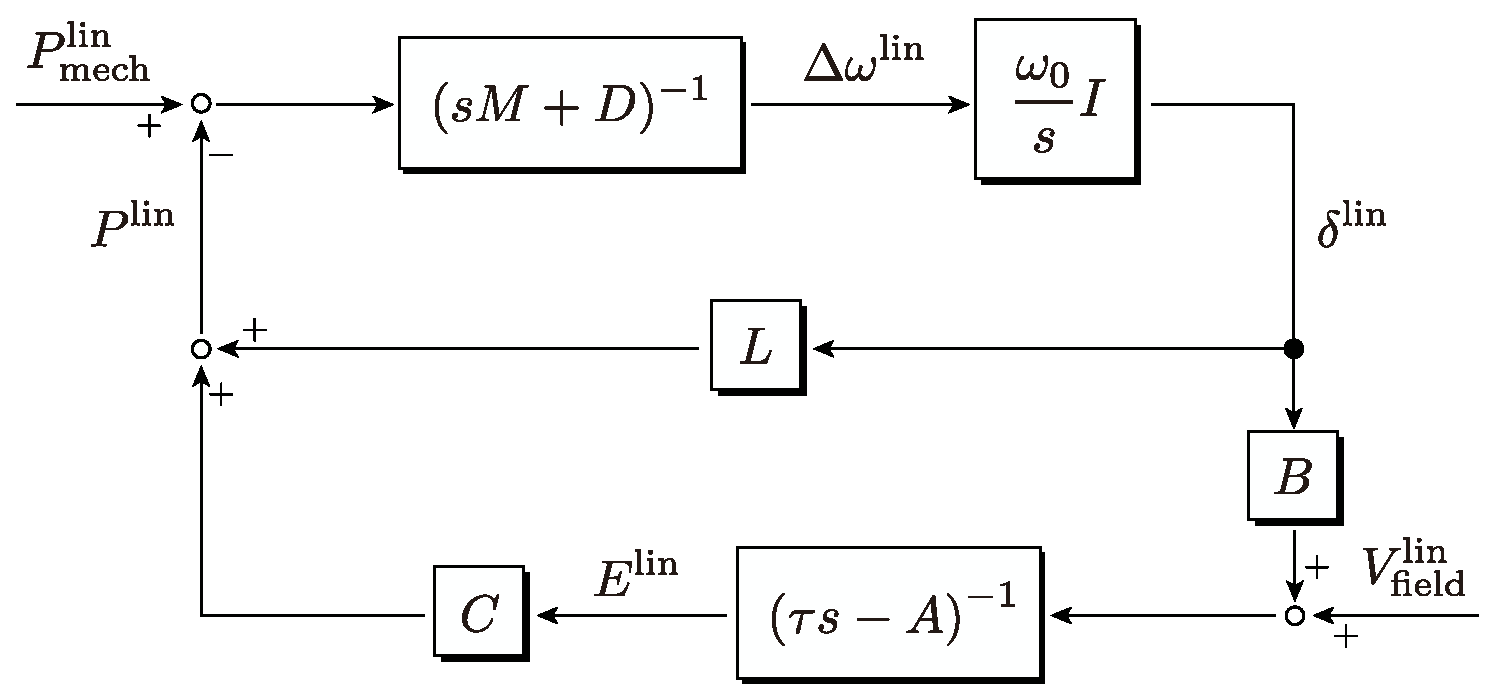
\includegraphics[width = .8\linewidth]{figs/blocklinsys3}
  \medskip
  \caption{\textbf{Block Diagram of Approximate Linear Model}}
  \label{fig:blocklinsys}
  \medskip
\end{figure}

\subsection{Stability analysis of approximate linear models}


\smallskip
\subsubsection{Stability of approximate linear models}

In this section, we consider numerically analyzing the stability of the
approximate linear model. Whether the approximate linear model of Equation
\ref{eq:lindyn} is stable or not is characterized by whether the internal states
of the generator groups return to the steady state satisfying the simultaneous
equations of Equation \ref{eq:kronss} in the event of a small disturbance in the
power system, such as temporary minor fluctuations in mechanical input or
excitation input of the generators, impedance values of the loads, current or
voltage values of the transmission lines, etc., from the reference values at the
steady state. In power system engineering, stability against such small
fluctuations is called \textbf{small signal stability}.

It should be noted that the stability of the approximate linear model of
Equation \ref{eq:lindyn} depends on the selection of the steady-state values of
the internal states of the generator groups $(\delta^{\star}, E^{\star})$ and
the steady-state values of external inputs $(P_{{\rm mech}}^{\star},V_{{\rm
field}}^{\star})$. Furthermore, changes in the admittance of the transmission
lines or the impedance of the loads alter the reduced conductance $G^{\rm
red}{ij}$ and reduced susceptance $B^{\rm red}{ij}$ of Equation \ref{eq:defkh}.
Therefore, the stability of the approximate linear model varies depending on
various model parameters mentioned above. The purpose of this section is to
numerically examine the relationship between the changes in these model
parameters and the stability of the approximate linear model.

\smallskip
\subsubsection{Stability analysis based on eigenvalues of the system matrix}

For the approximate linear model in Equation \ref{eq:lindyn}, if we
appropriately choose the steady-state values $(\delta^{\star},E^{\star})$ of the
internal states as parameters, then the system matrix $(L,A,B,C)$ in Equation
\ref{eq:sysmats} and the steady-state values $(P_{{\rm mech}}^{\star},V_{{\rm
field}}^{\star})$ of the external inputs satisfying Equation \ref{eq:kronss} are
determined dependently. Here, we consider setting

\[
  P_{{\rm mech}i}(t)=P_{{\rm mech}i}^{\star},\qquad
  V_{{\rm field}i}(t)
  =
  V_{{\rm field}i}^{\star},\qquad 
  \forall t\geq 0
\]
for all $i \in \mathcal{I}{\rm G}$ in the nonlinear differential equation system
model in Equation \ref{eq:krondyn}. We then assess the stability of the system
using the eigenvalues of the system matrix.

This means that in the approximate linear model of Equation \ref{eq:lindyn} the
following values are set:

\[
  P_{{\rm mech}}^{\rm lin}(t)
  =0,\qquad
  V_{{\rm field}}^{\rm lin}(t)
  =0
  ,\qquad 
  \forall t\geq 0
\]

In the following, under this assumption, we analyze the stability of an
autonomous approximate linear model with input set identically to zero, given
by:

\begin{equation}\label{eq:lindynu0}
  \mat{
    \dot{\delta}^{\rm lin} \\
    \Delta \dot{\omega}^{\rm lin} \\
    \dot{E}^{\rm lin}
  }
  =
  \underbrace{
    \mat{
      0 & \omega_0 I & 0\\
      -M^{-1}L & -M^{-1}D & -M^{-1}C \\
      \taud^{-1} B & 0 & \taud^{-1} A
    }
  }_{\Psi}
  \mat{
    \delta^{\rm lin} \\
    \Delta \omega^{\rm lin} \\
    E^{\rm lin}
  }
\end{equation}

Specifically, by examining the sign of the real part of the eigenvalues of the
matrix $\Psi$, we can determine the stability of this approximate linear model.
However, it should be noted that $\Psi$ generally has at least one zero
eigenvalue. In fact, from the structure of the matrices $L$ and $B$ in equation
\ref{eq:sysmats}, we have:

\begin{equation}\label{eq:LBker}
  L  \mathds{1} = 0
  ,\qquad
  B  \mathds{1} =0
\end{equation}

Therefore, for any model parameters, we have:

\[
  \Psi v=0 ,\qquad
  v:=\mat{
    \mathds{1} \\
    0 \\
    0
  }
\]

This means that $v$ is an eigenvector of $\Psi$ corresponding to a zero
eigenvalue. If the real parts of all eigenvalues, except for the zero
eigenvalue, are negative, then for any initial value, the solution trajectory of
Equation \ref{eq:lindynu0} satisfies:

\begin{equation}\label{eq:linmconv}
  \lim_{t\rightarrow \infty}\delta^{\rm lin}(t)= c_0  \mathds{1},\qquad
  \lim_{t\rightarrow \infty}\Delta \omega^{\rm lin}(t)=0 ,\qquad
  \lim_{t\rightarrow \infty} E^{\rm lin}(t)=0
\end{equation}

Here, $c_0$ is a constant determined by the initial value. Note that the value
of $c_0$ does not make a significant difference in the analytical results. This
is because in the differential equation system model of Equation
\ref{eq:krondyn_}, the rotor angle $\delta_i$ of a generator has meaning only in
relation to the difference between the rotor angle $\delta_j$ of other
generators. Specifically, if $(\delta^{\star},E^{\star})$ satisfies the system
of equations in equation \ref{eq:kronss} for a certain $(P_{{\rm
mech}}^{\star},V_{{\rm field}}^{\star})$, then $(\delta^{\star}+c_0
\mathds{1},E^{\star})$ also satisfies the same system of equations. Therefore,
$\delta^{\star}$ and $\delta^{\star}+c_0 \mathds{1}$ are essentially equivalent
steady-state values where all generator rotor angles are rotated by the same
amount of $c_0$. Equation \ref{eq:linmconv} means the asymptotic convergence of
solution trajectories to these essentially equivalent steady-state values.

\section{stability analysis of approximate linear models using numerical
calculations}\label{sec:numlinsta}

\subsection{Implementation of approximate linearization using a group of
partitioned modules}

In this section, we explain the implementation method for obtaining an
approximate linear model numerically. Specifically, we describe how to add the
functionality of linearization to the program that has been segmented into
module groups as explained in Sections \ref{sec:powfcal} and
\ref{sec:timerescal}.

In the numerical simulation program of the power system created in Section
\ref{sec:timerescal}, the following state and output equations are implemented
for each device as differential and algebraic equations, respectively:

\[
  \dot{x}_i = f_i^{(1)}(x_i, \bm V_i, \bm I_i, u_i)
  ,\qquad
  0 = f_i^{(2)} (x_i, \bm V_i, \bm I_i, u_i)
\]

In the following, we derive the approximate linear model in the vicinity of the
equilibrium point $(x_i^\star, \bm V_i^\star, \bm I_i^\star, u_i^\star)$ for the
device of interest. Specifically, we explain the implementation method of the
linear approximation function to the program that has been partitioned into the
module group described in Sections \ref{sec:powfcal} and \ref{sec:timerescal}.

For the numerical simulation program of the power system created in Section
\ref{sec:timerescal}, differential equations for the state and algebraic
equations for the output are implemented for each device as:

\[
  \dot{x}_i = f_i^{(1)}(x_i, \bm V_i, \bm I_i, u_i)
  ,\qquad
  0 = f_i^{(2)} (x_i, \bm V_i, \bm I_i, u_i)
\]

We consider the linearization of the functions $f_i^{(1)}$ and $f_i^{(2)}$ as
follows:

\begin{align}
  \hspace{-1mm}  f_i^{(1)} (x_i, \bm V_i, \bm I_i,u_i) &\approx A_i (x_i-x_i^\star) + B_{u_i}u_i\notag\\
    &+ B_{\bm{V}_i} \! \mat{
      \real[\bm V_i-\bm V^\star]\\ \imag[\bm V_i-\bm V^\star]
    }
    + 
    B_{\bm{I}_i} \! \mat{
      \real[\bm I_i-\bm I_i^\star]\\\imag[\bm I_i-\bm I_i^\star]
    }\label{eq:f_lin}\\
  \hspace{-1mm} f_i^{(2)} (x_i, \bm V_i, \bm I_i,u_i) &\approx C_i (x_i-x_i^\star) + D_{u_i}u_i\notag\\
    &+ 
    D_{\bm{V}_i}  \! \mat{
      \real[\bm V_i-\bm V^\star]\\ \imag[\bm V_i-\bm V^\star]
    }
    + D_{\bm{I}_i}  \! \mat{
      \real[\bm I_i-\bm I_i^\star]\\\imag[\bm I_i-\bm I_i^\star]\label{eq:g_lin}
    }
\end{align}

A system of simultaneous equations for each machine and algebraic equations for
the entire power system can be used to obtain an expression using ordinary
differential equations for the approximate linear model by eliminating all $\bm
V_i -\bm V^\star_i$ and $\bm I_i-\bm I_i^\star$, where $i \in {1,\ldots,N}$, as
follows:

\[
  \bm I_i - \bm I_i^\star = \sum_{j=1}^N \bm Y_{ij} (\bm{V}_j -\bm V^\star_j )
  ,\qquad
  i \in \{1,\ldots,N\}
\]

Here, $\bm{Y}_{ij}$ represents the $(i,j)$th element of the admittance matrix
$\bm{Y}$. Let us check the specific implementation method with the following
example.

\begin{example}[Implementation of Approximate Linear Model]

Equations \ref{eq:f_lin} and \ref{eq:g_lin} depend on the dynamic
characteristics of the device, so it is natural to implement the calculation of
coefficient matrices such as $A_i$ and $B_{u_i}$ in the classes of devices such
as generators and loads in the implementation example of Section
\ref{sec:powfcal}. For example, in the generator model:

\begin{flalign*}
  &\quad
  A_i = \mat{
  0 & \omega_0 & 0\\
  0 & -\tfrac{D_i}{M_i} & 0\\
  - \tfrac{1}{\tau_i}( \tfrac{X_i}{X_i'}-1)|\bm V_i^\star|\sfsin(\delta_i^\star-\angle\bm V_i^\star) &
  0& - \tfrac{X_i}{\tau_i X'_i}
  }
  &
  \end{flalign*}
  \begin{flalign*}
  &\quad
  B_{u_i} = \mat{
    0 \\ \tfrac{1}{M_i} \\ 0
  }
  ,\qquad
  B_{\bm{V}_i} = \mat{
    0 & 0\\ - \tfrac{\real [ \bm{I}_i^\star] }{M_i}  & - \tfrac{\imag[ \bm{I}_i^\star] }{M_i}\\
  \tfrac{1}{\tau_i}( \tfrac{X_i}{X_i'}-1) \sfcos \delta_i^\star& \tfrac{1}{\tau_i}( \tfrac{X_i}{X_i'}-1) \sfsin\delta_i^\star
  }
  &
\end{flalign*}
\begin{flalign*}
  &\quad
  B_{\bm{I}_i} = \mat{
    0 & 0\\ -\tfrac{\real [ \bm{V}_i^\star] }{M_i} & -\tfrac{\imag [ \bm{V}_i^\star] }{M_i}\\
  0 & 0 
  }
  ,\qquad
  C_i = \mat{
  E_i^\star\sfcos\delta^\star_i & 0 & \sfsin(\delta_i^\star)\\
  E_i^\star\sfsin\delta^\star_i & 0 & -\sfcos(\delta_i^\star)\\
  }
  &
\end{flalign*}
\begin{flalign*}
  &\quad
  D_{u_i} = \mat{0 \\ 0}
  ,\qquad
  D_{\bm{V}_i} = \mat{
    0 & -1\\ 1 & 0
  }
  ,\qquad
  D_{\bm{I}_i} =  \begin{bmatrix}
    -X_i' & 0\\0 & -X_i'
  \end{bmatrix}
  &
\end{flalign*}

If the calculation of these coefficient matrices is added to the
\verb|generator| class as a method named \verb|get_linear_matrix|, the program
\ref{program:generator_matrix} is obtained.

\smallskip
\begin{lstlisting}[language=Matlab, caption=generator.m, label={program:generator_matrix}]
classdef generator < handle
  
  properties
(Same as lines 4-11 in program 3-23)
    x_equilibrium
    V_equilibrium
    I_equilibrium
  end
  
  methods

(Same as lines 7 through 21 in program 3-34)

    function x_equilibrium = set_equilibrium(obj, V, I, P, Q)

(Same as lines 10 through 23 of program 3-28)

      obj.x_equilibrium = x_equilibrium;
      obj.V_equilibrium = V;
      obj.I_equilibrium = I;
    end
    
    function [A, Bu, BV, BI, C, Du, DV, DI] =...
        get_linear_matrix(obj)
      
      X = obj.X;
      X_prime = obj.X_prime;
      D = obj.D;
      M = obj.M;
      tau = obj.tau;
      
      omega0 = obj.omega0;
      delta = obj.x_equilibrium(1);
      E = obj.x_equilibrium(3);
      V = obj.V_equilibrium;
      Vabs = abs(obj.V_equilibrium);
      Vangle = angle(obj.V_equilibrium);
      I = obj.I_equilibrium;
      A = [0, omega0, 0;
        0, -D/M, 0;
        -(X/X_prime-1)*Vabs*sin(delta-Vangle)/tau,...
        0, -X/X_prime/tau];
      Bu = [0; 1/M; 0];
      BV = [0, 0;
        -real(I)/M, -imag(I)/M;
        (X/X_prime-1)*cos(delta)/tau,...
        (X/X_prime-1)*sin(delta)/tau];
      BI = [0, 0;
        -real(V)/M, -imag(V)/M;
        0, 0];
      C = [E*cos(delta), 0, sin(delta);
        E*sin(delta), 0, -cos(delta)];
      Du = [0; 0];
      DV = [0, -1; 1, 0];
      DI = -X_prime*eye(2);
    end

  end

end
\end{lstlisting}

In Program \ref{program:generator_matrix}, lines 18 to 20 in
\verb|set_equilibrium| store information about the equilibrium point used in the
calculation of the approximate linear model.

If implemented similarly for the constant impedance load model, the program
\ref{program:load_matrix} is obtained.

\smallskip
\begin{lstlisting}[language=Matlab, caption=load\_impedance.m, label={program:load_matrix}]
classdef load_impedance < handle
  
  properties
    z
    I_equilibrium
  end
  
  methods

(Same as lines 7 through 18 in program 3-35)
   
    function x_equilibrium = set_equilibrium(obj, V, I, P, Q)
      x_equilibrium = [];
      obj.z = -V/I;
      obj.I_equilibrium = I;
    end
    
    function [A, Bu, BV, BI, C, Du, DV, DI] =...
        get_linear_matrix(obj)
      
      A = [];
      Bu = zeros(0, 2);
      BV = zeros(0, 2);
      BI = zeros(0, 2);
      C = zeros(2, 0);
      I = obj.I_equilibrium;
      z = obj.z;
      Du = [real(z)*real(I), imag(z)*imag(I);
        real(z)*imag(I), imag(z)*real(I)];
      DV = eye(2);
      DI = [real(z), -imag(z); imag(z), real(z)];
    end
    
  end
  
end
\end{lstlisting}

By using the class of equipment such as modified generators and loads, the
function for obtaining an approximate linear model can be described as shown in
Program \ref{program:linearization}.

\smallskip
\begin{lstlisting}[language=Matlab, caption=get\_linear\_model.m, label={program:linearization}]
function sys = get_linear_model(a_component, Y)

  A = cell(numel(a_component), 1);
  Bu = cell(numel(a_component), 1);
  BV = cell(numel(a_component), 1);
  BI = cell(numel(a_component), 1);
  C = cell(numel(a_component), 1);
  Du = cell(numel(a_component), 1);
  DV = cell(numel(a_component), 1);
  DI = cell(numel(a_component), 1);

  for k = 1:numel(a_component)
    component = a_component{k};
    [A{k}, Bu{k}, BV{k}, BI{k}, C{k}, Du{k}, DV{k}, DI{k}] =...
      component.get_linear_matrix();
  end

  A = blkdiag(A{:});
  Bu = blkdiag(Bu{:});
  BV = blkdiag(BV{:});
  BI = blkdiag(BI{:});
  C = blkdiag(C{:});
  Du = blkdiag(Du{:});
  DV = blkdiag(DV{:});
  DI = blkdiag(DI{:});

  Ymat = zeros(size(Y, 1)*2, size(Y, 2)*2);
  Ymat(1:2:end, 1:2:end) = real(Y);
  Ymat(2:2:end, 1:2:end) = imag(Y);
  Ymat(1:2:end, 2:2:end) = -imag(Y);
  Ymat(2:2:end, 2:2:end) = real(Y);

  nx = size(A, 1);

  A11 = A;
  A12 = [BV, BI];
  A21 = [C; zeros(size(Ymat, 1), nx)];
  A22 = [DV, DI; Ymat, -eye(size(Ymat))];

  B1 = Bu;
  B2 = [Du; zeros(size(Ymat, 1), size(Du, 2))];


  Aout = A11 - A12/A22*A21;
  Bout = B1 - A12/A22*B2;
  Cout = eye(nx);
  Dout = 0;

  sys = ss(Aout, Bout, Cout, Dout);

end
\end{lstlisting}

In lines 12 to 16 of Program \ref{program:linearization}, the coefficient matrix
of the approximate linear model is obtained from each equipment. Additionally,
by eliminating the voltage and current phases of all buses from lines 27 to 47,
an expression for the approximate linear model's system of ordinary differential
equations is obtained.

The approximate linear model can be used as follows by using Program
\ref{program:linearization}.


\smallskip
\begin{lstlisting}[language=Matlab, caption=main\_linearization.m, label={program:main_linearization}]
(Same as lines 1 through 23 in Program 3-30)

sys = get_linear_model(a_component, Y);

sys = sys(2, 1);
nyquist(sys)
\end{lstlisting}

In this example, an approximate linear model is constructed in line 5 with the
mechanical input $P_{{\rm mech}1}$ of generator 1 as input and the frequency
deviation $\Delta\omega_1$ of generator 1 as output. In addition, a Nyquist plot
is drawn in line 6.
\end{example}

In the mathematical analysis of Section \ref{sec:linaproxt}, an approximate
linear model is derived from a nonlinear system of ordinary differential
equations where all buses are Kron reduced. On the other hand, in the numerical
implementation of this section, the nonlinear differential-algebraic equation
system is first linearized, and then Kron reduction is applied to construct the
ordinary differential equation system. It should be noted that this is because
in the power system model with Kron reduction, expressions generally involve a
mixture of information about equipment, buses, and transmission lines.

To increase the readability and expandability of the program, it is important to
modularize each element appropriately, as in the implementation of this section.

\subsection{Numerical analysis of small signal stability}

Let us perform a stability analysis based on approximate linearization for an
actual electrical power system model consisting of three generators.

%\begin{figure}[t]
%\centering
%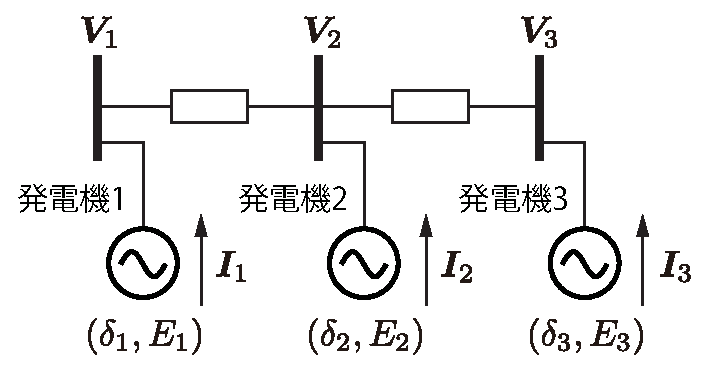
\includegraphics[width = .5\linewidth]{figs/gen3ex}
%\medskip
%\caption{\textbf{3つの発電機からなる電力系統モデル}}
%\label{fig:3genex}
%\medskip
%\end{figure}
%
%\begin{figure}[t]
%  \centering
%  {
%  \begin{minipage}{0.49\linewidth}
%    \centering
%    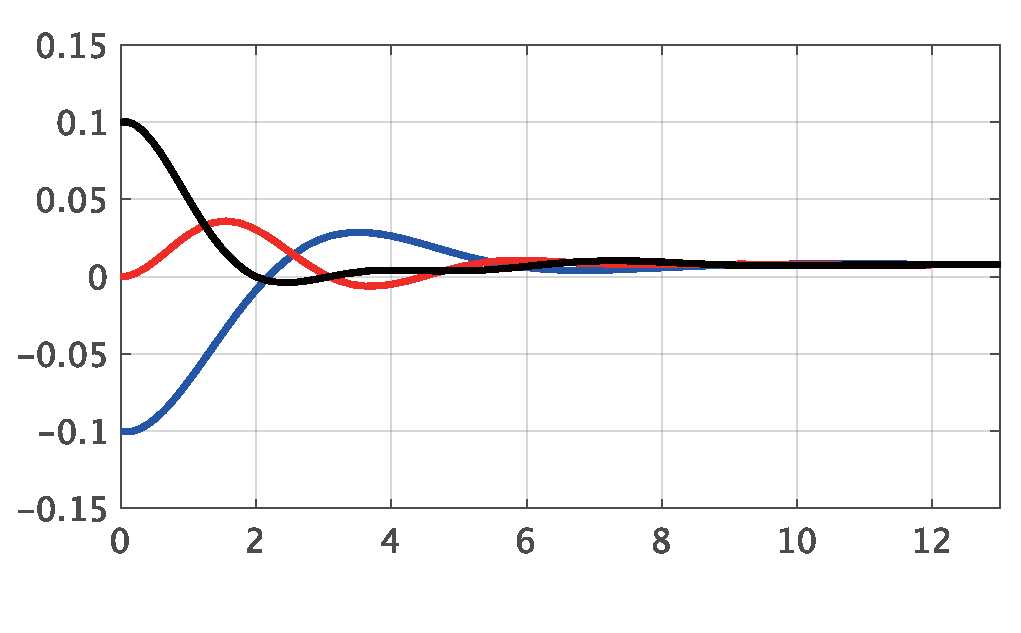
\includegraphics[width = 1.0\linewidth]{figs/delta}
%    \subcaption{ $\delta^{\rm lin}$ }
%    \medskip
%  \end{minipage}
%  \begin{minipage}{0.49\linewidth}
%    \centering
%    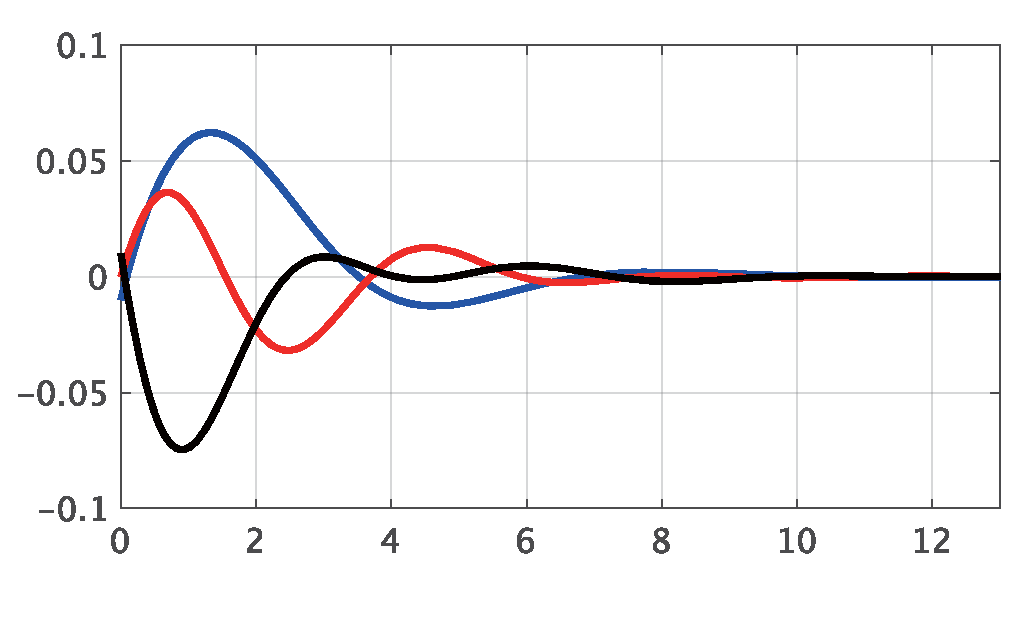
\includegraphics[width = 1.0\linewidth]{figs/omega}
%    \subcaption{ $\Delta \omega^{\rm lin}$ }
%    \medskip
%  \end{minipage}
%%  \begin{minipage}{0.32\linewidth}
%    \centering
%    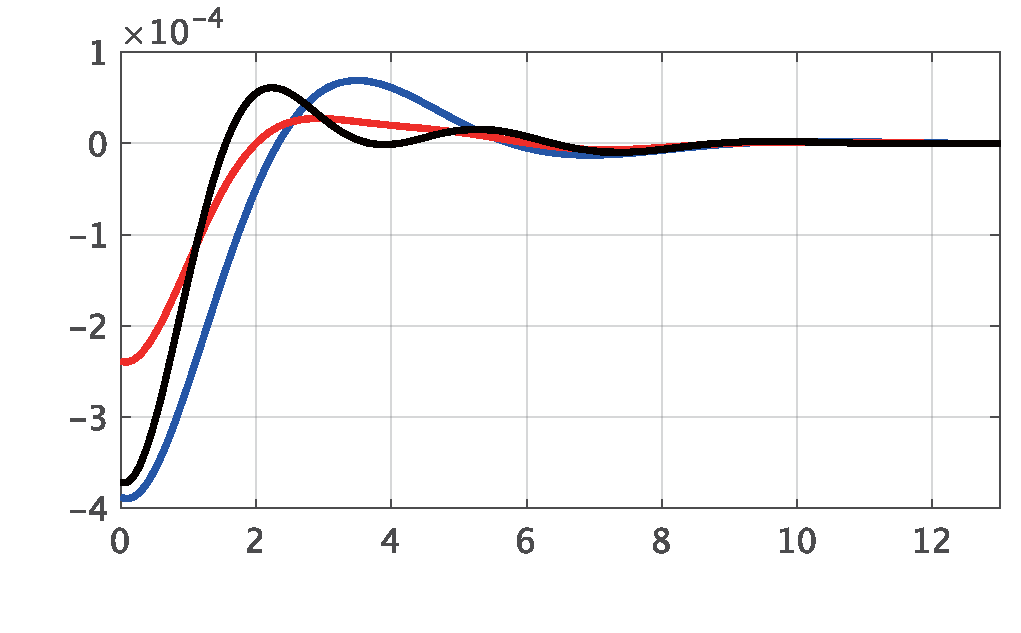
\includegraphics[width = .49\linewidth]{figs/E}
%    \subcaption{ $E^{\rm lin}$ }
%%  \end{minipage}
%  }
%  \medskip
%  \caption{\textbf{近似線形モデルの初期値応答}}
%  \label{fig:timeex}
%\medskip
%\end{figure}


\begin{figure}[t]
  \centering
  {
  \begin{minipage}{0.49\linewidth}
    \centering
    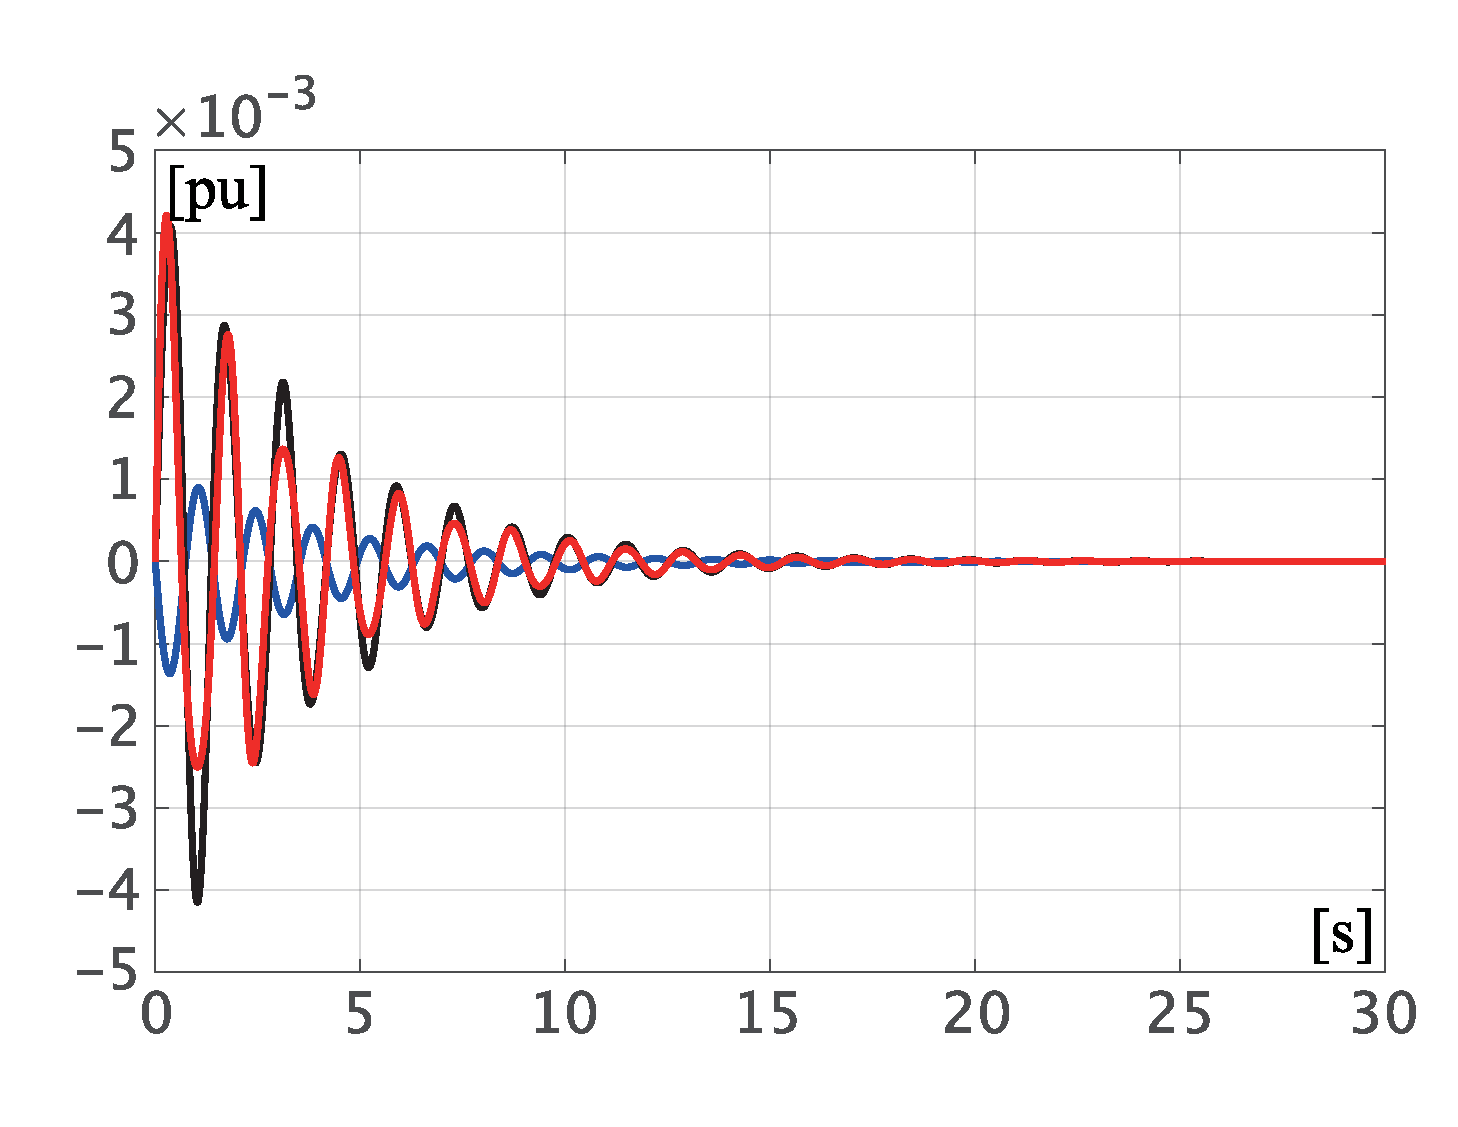
\includegraphics[width = 1.0\linewidth]{figs/Domegalin}
    \subcaption{ $\Delta \omega^{\rm lin}$ }
    \medskip
  \end{minipage}
  \begin{minipage}{0.49\linewidth}
    \centering
    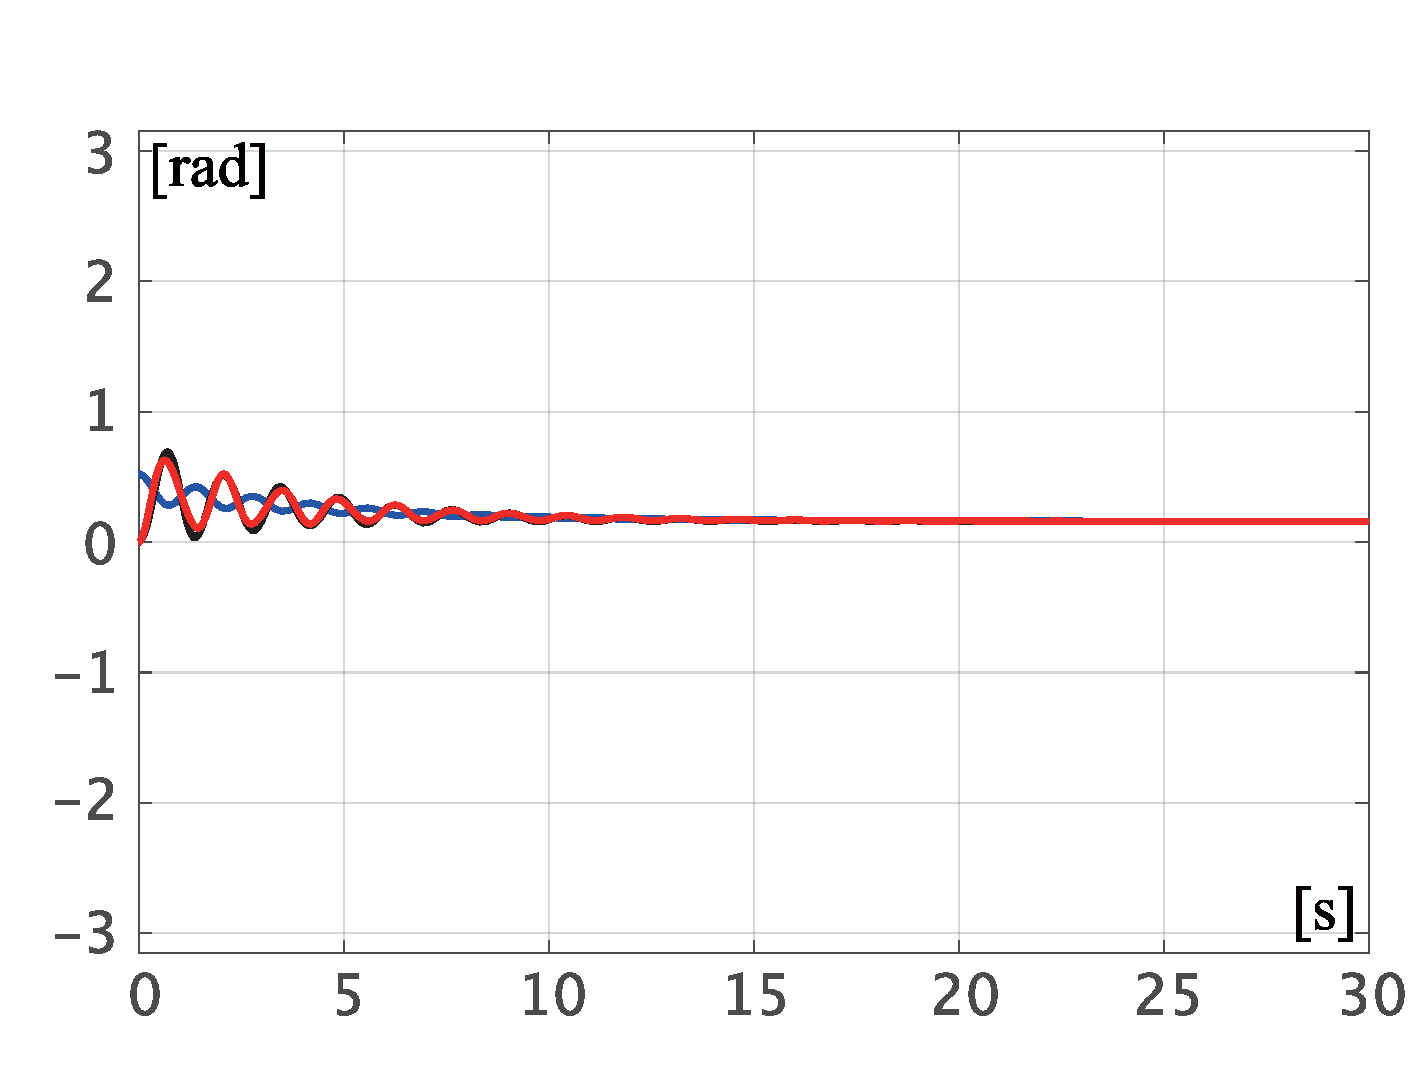
\includegraphics[width = 1.0\linewidth]{figs/deltalin}
    \subcaption{ $\delta^{\rm lin}$ }
    \medskip
  \end{minipage}
 \begin{minipage}{0.49\linewidth}
    \centering
    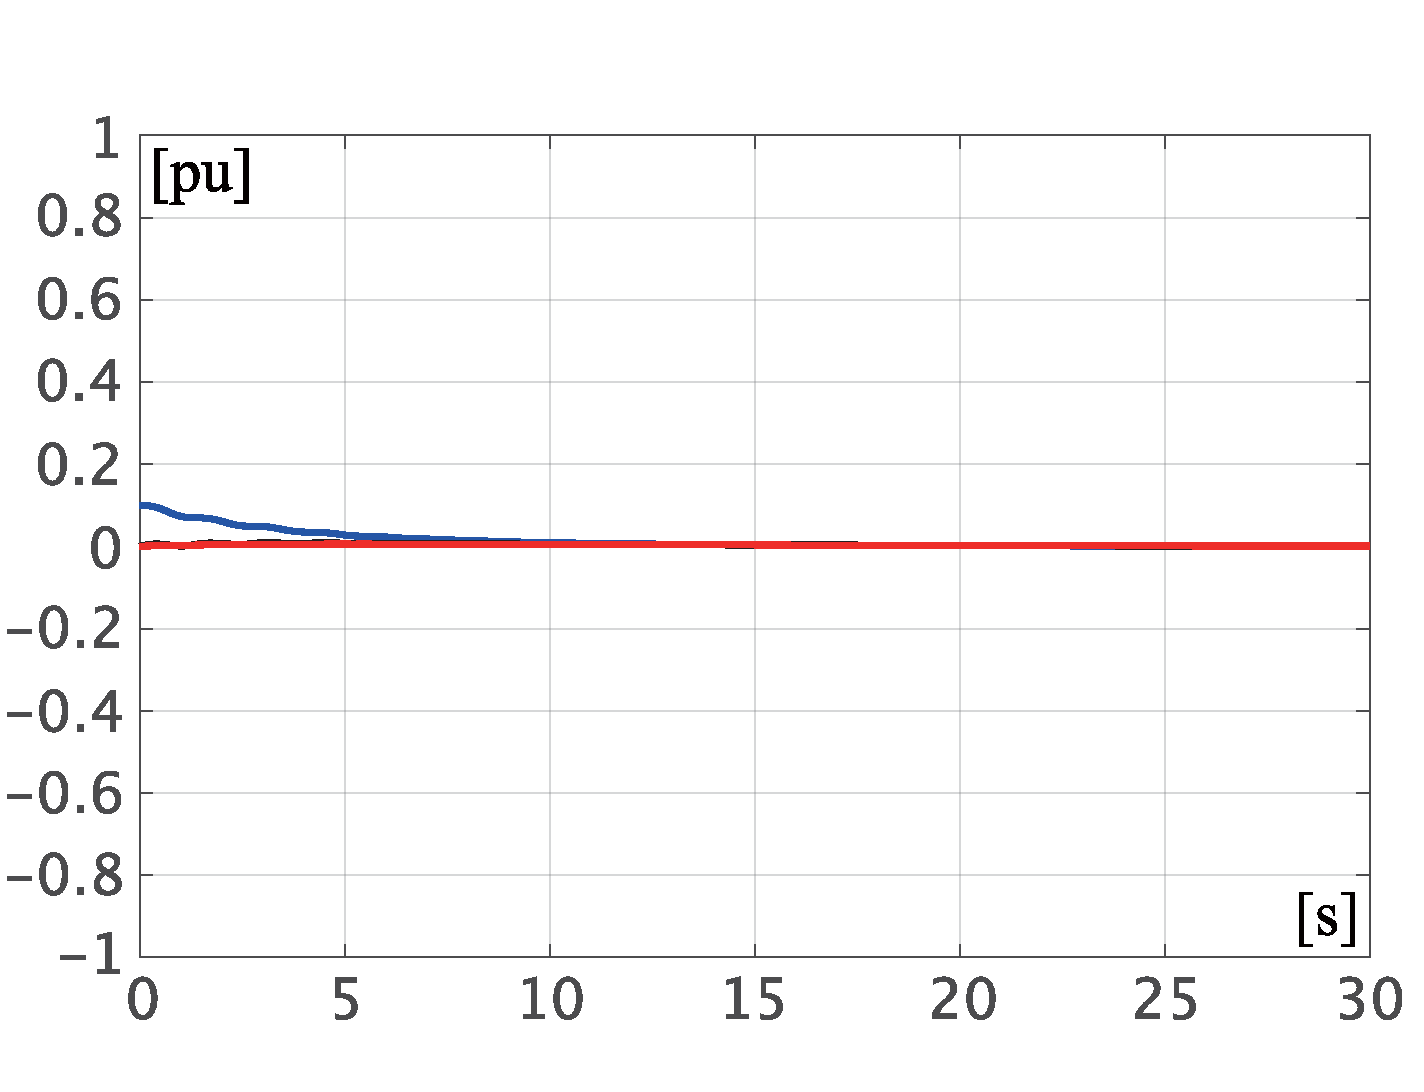
\includegraphics[width = 1.0\linewidth]{figs/Elin}
    \subcaption{ $E^{\rm lin}$  }
    \medskip
  \end{minipage}
  \begin{minipage}{0.49\linewidth}
    \centering
    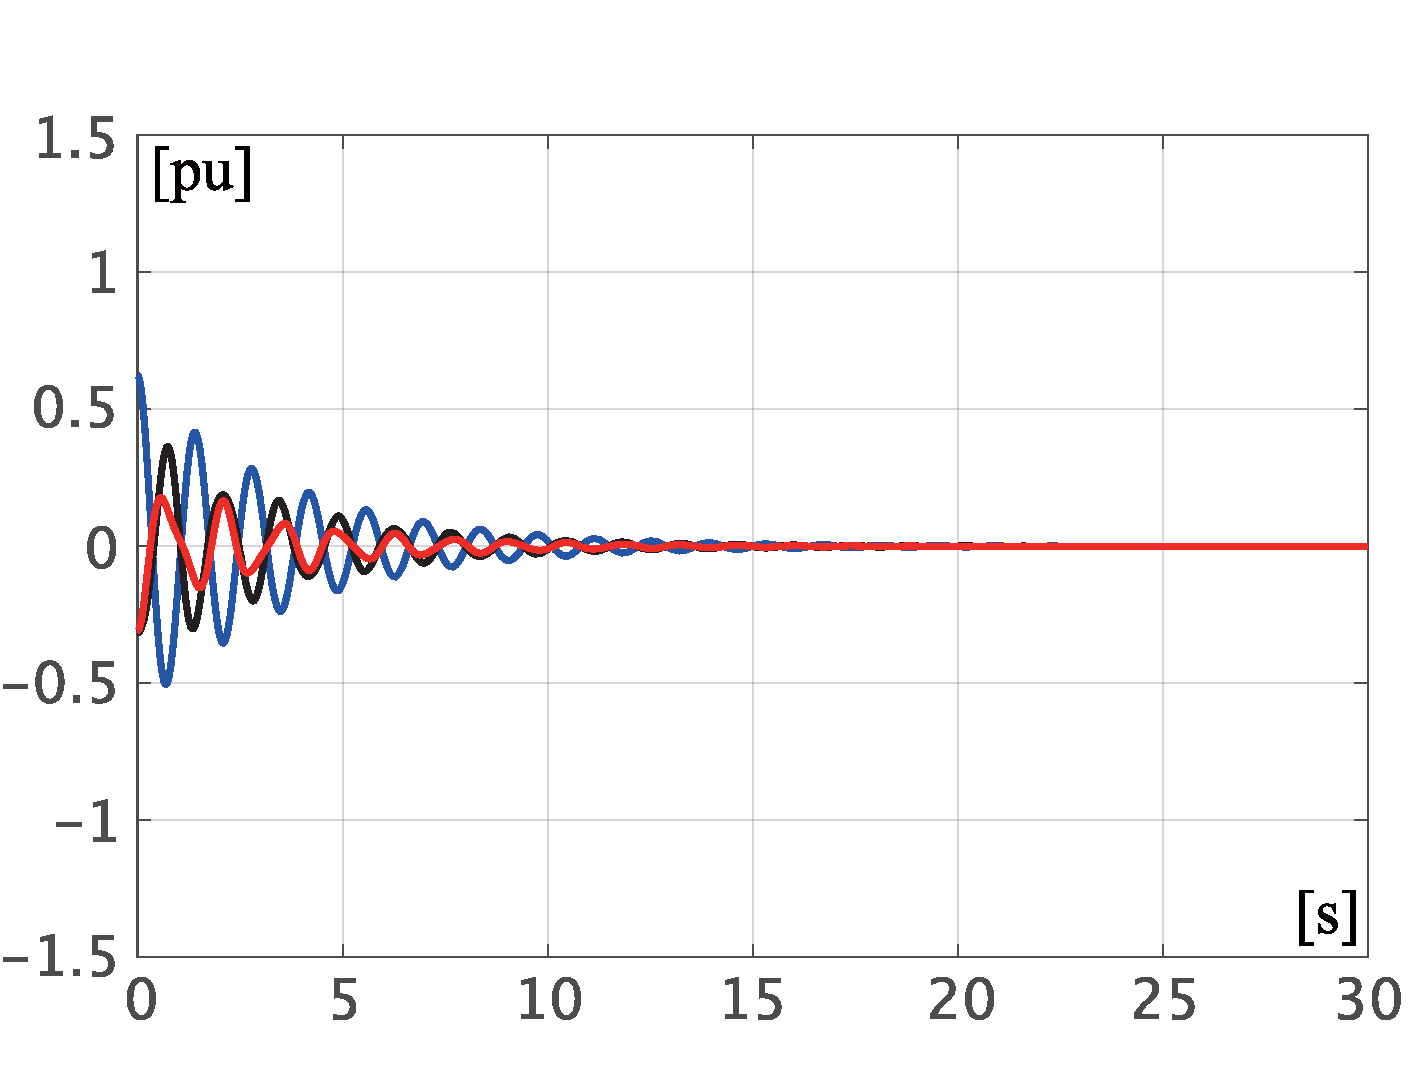
\includegraphics[width = 1.0\linewidth]{figs/Plin}
    \subcaption{ $P^{\rm lin}$ }
    \medskip
  \end{minipage}
  }
  \medskip
  \caption{\textbf{Initial value response of approximate linear model}
  \\  \centering(Blue: Generator 1, Black: Generator 2, Red: Generator 3)}
  \label{fig:timeex}
\medskip
\end{figure}


%\begin{figure}[t!]
%\centering
%  {
%    \centering
%    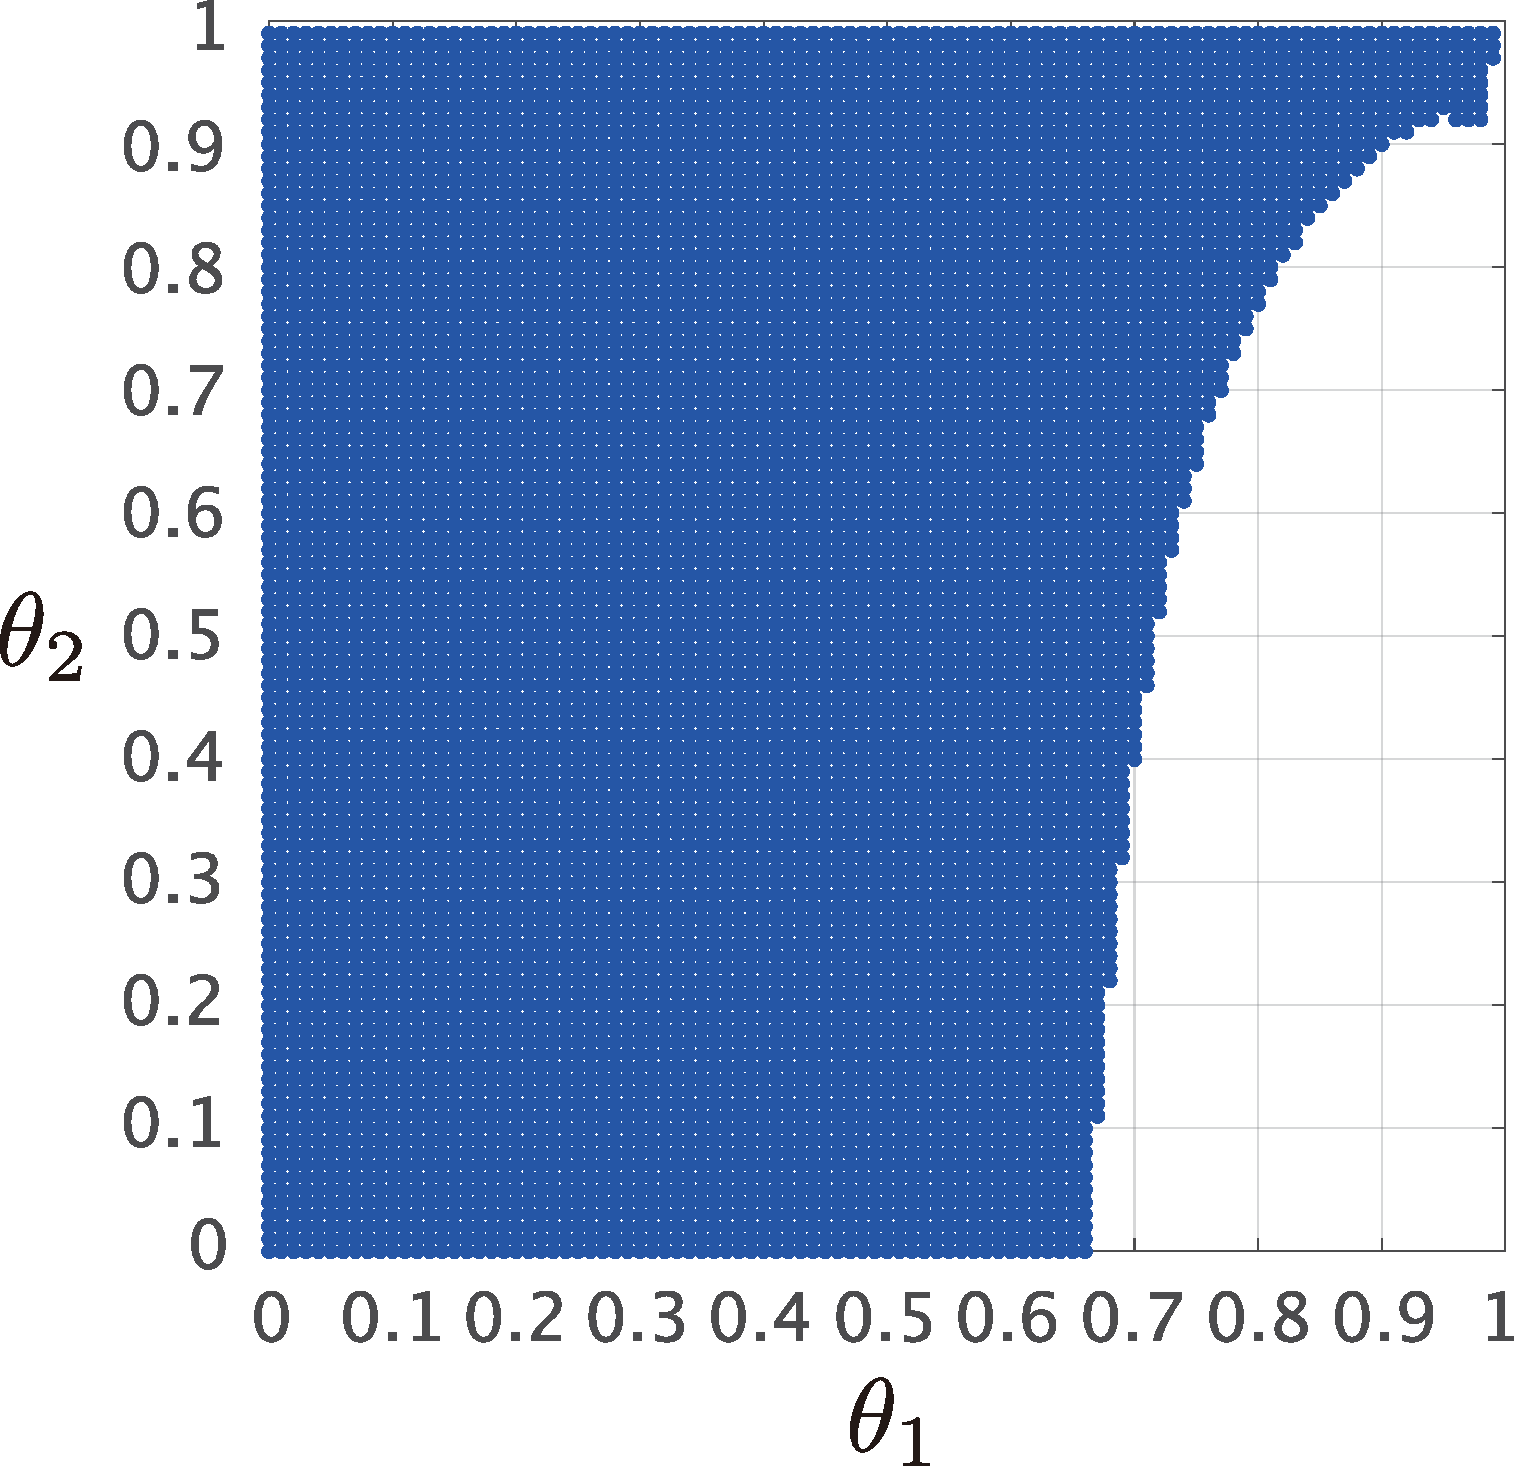
\includegraphics[width = .4\linewidth]{figs/gam01}
%    \subcaption{ $\gamma=0.1$ }
%    \centering
%    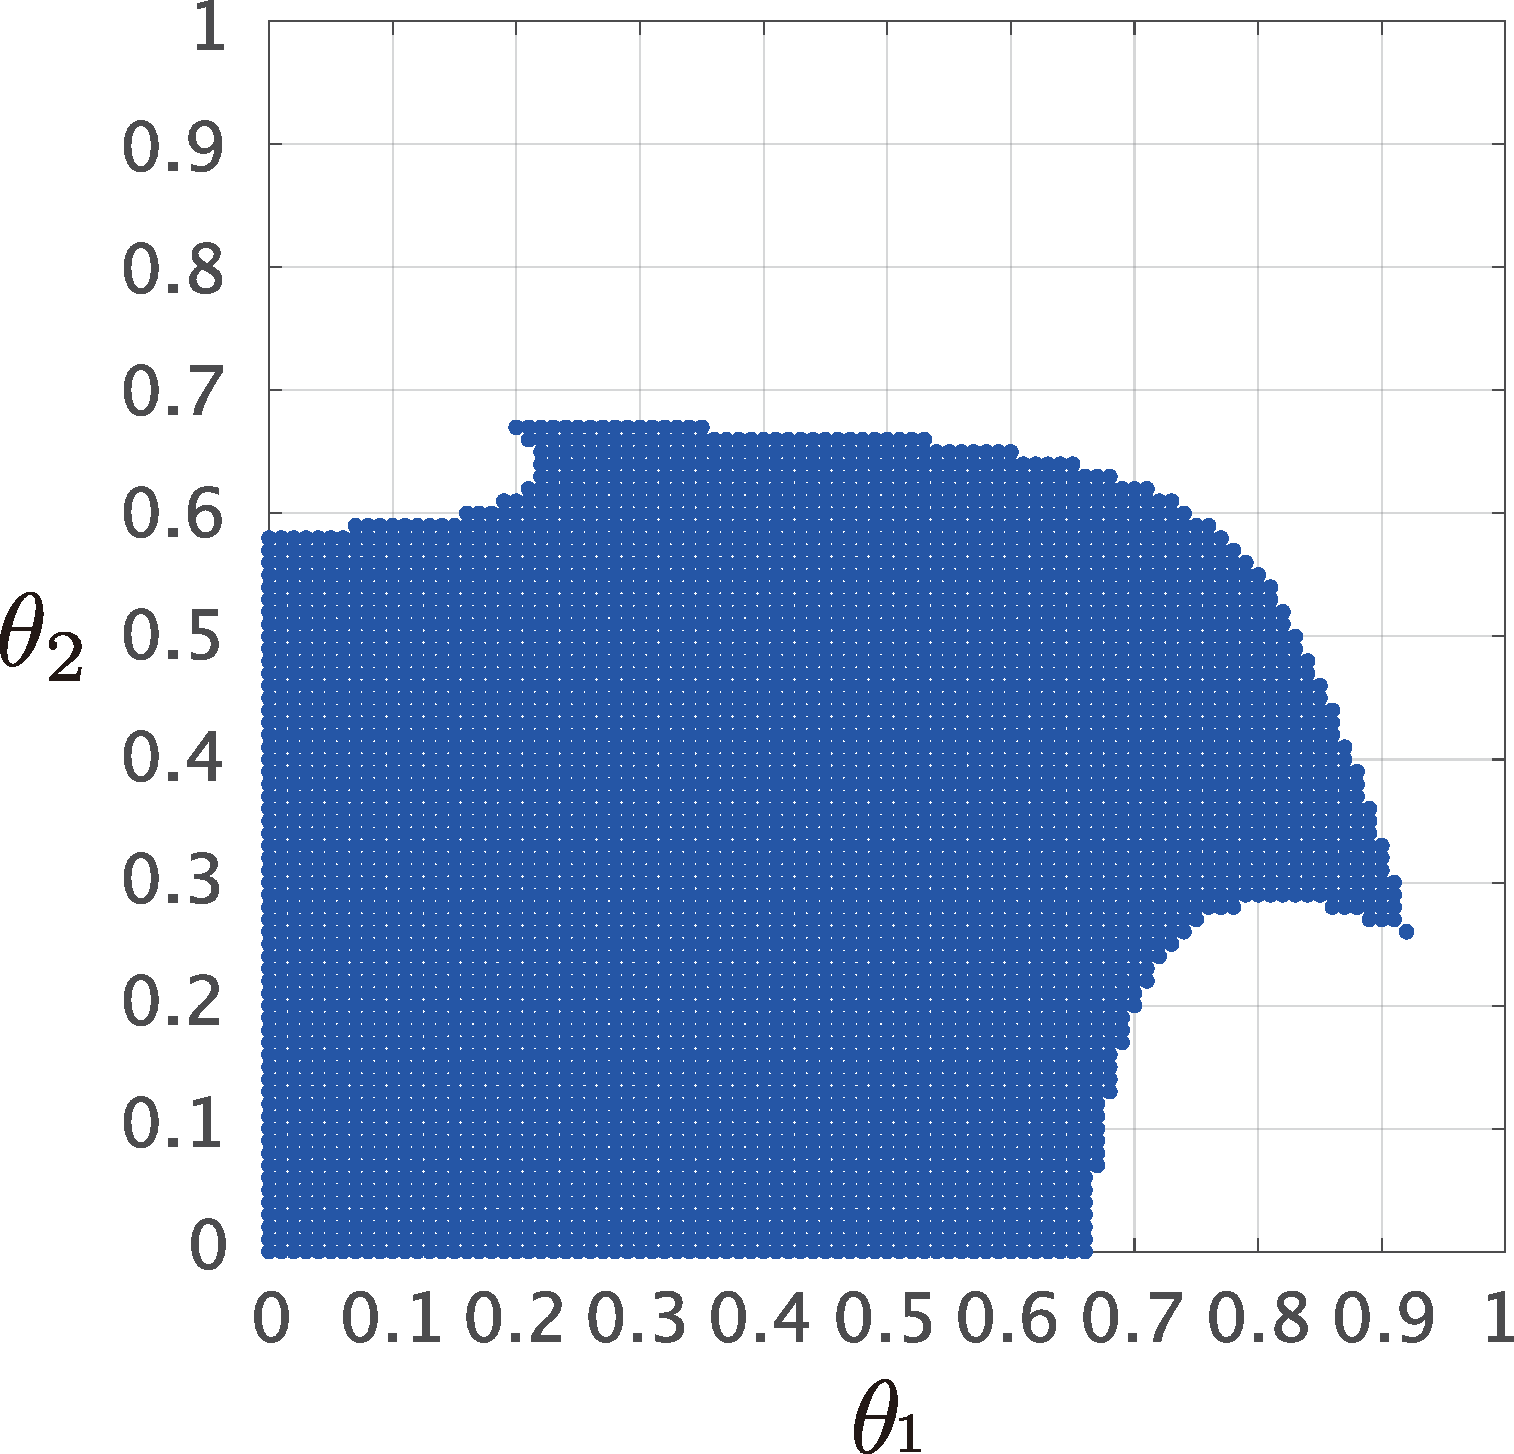
\includegraphics[width = .4\linewidth]{figs/gam2}
%    \subcaption{ $\gamma=2$ }
%    \centering
%    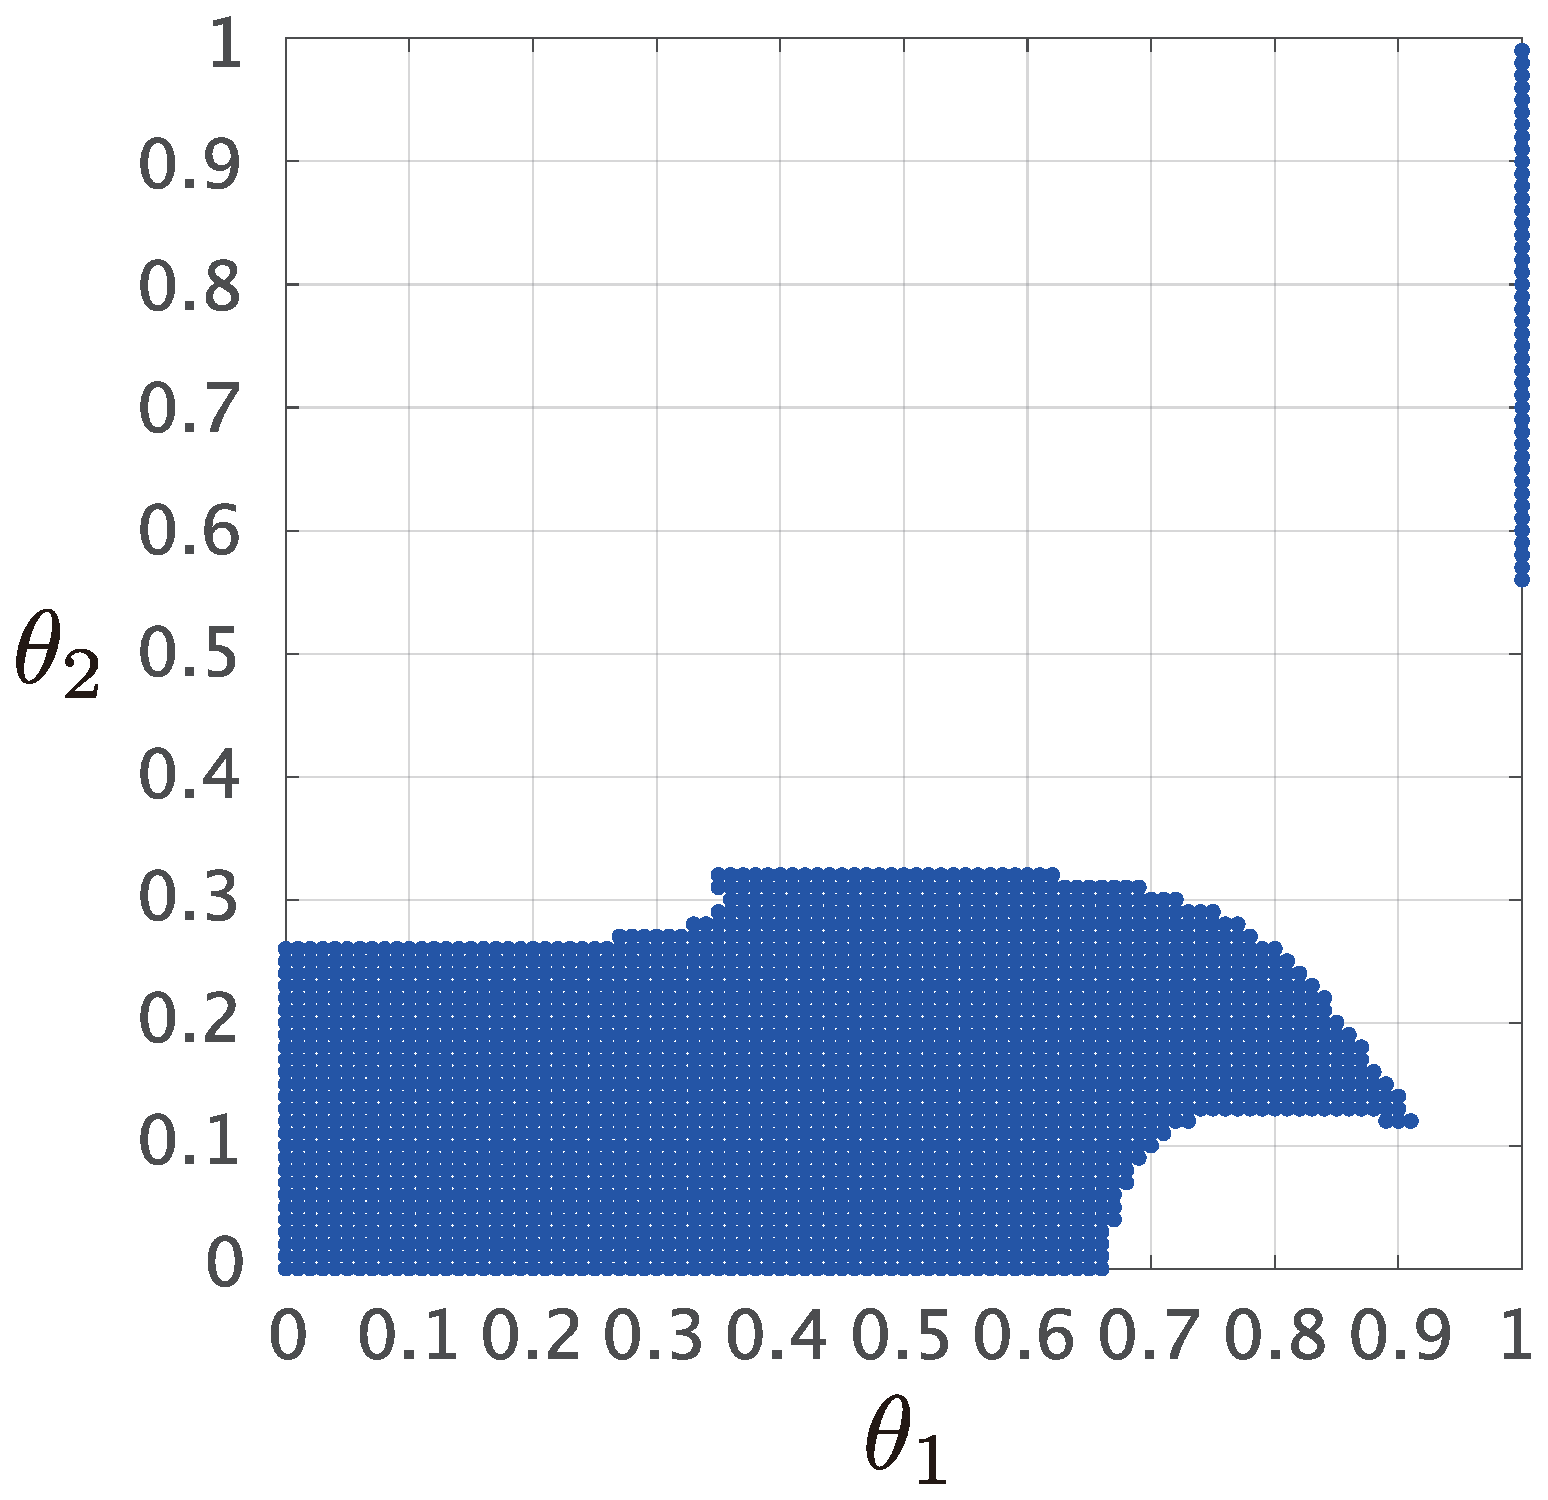
\includegraphics[width = .4\linewidth]{figs/gam5}
%    \subcaption{ $\gamma=5$ }
%  }
%\caption{近似線形モデルが安定となるパラメータの領域}
%\label{fig:gamsta}
%\medskip
%\end{figure}



\begin{example}{Numerical stability analysis of the linearized model}\label{ex:linsyssim}
Let us consider an electrical power system model consisting of three generators
discussed in the Example \ref{ex:Kronode}. The constant of the generators and
transmission lines are set to the same value as in the Example \ref{ex:Kronode},
and a linear approximation model for Equation \ref{eq:lindynu0} is derived with
the approximate of the steady value shown in \ref{table:gensteady}. Figure
\ref{fig:timeex} shows the time response When the initial values are set as
follows to correspond to Equation \ref{eq:exdelE0}:

\begin{equation}\label{eq:linmini}
  \delta^{\rm lin}(0)
  =
  \mat{
    \tfrac{\pi}{6} \\
    0 \\
    0
  },\quad
  \Delta \omega^{\rm lin}(0)
  =
  \mat{
    0 \\
    0 \\
    0
  },\quad
  E^{\rm lin}(0)
  =
  \mat{
    0.1 \\
    0 \\
    0
  }
\end{equation}

The blue, black, and red lines represent generators 1, 2, and 3, respectively.
From this figure, we can see that the internal state of the generator group
converges asymptotically as given in \eqref{eq:linmconv}.  Moreover, it
approximately reproduces the initial value response of the nonlinear model shown
in Fig. \ref{fig:Kron0}.

Next, we parameterize the constants and steady-state values of the generators
and transmission lines to analyze the stability of the resulting approximate
linear model. For the generator constants, we compare the cases where all the
damping coefficients are set to 10 and where they are set to 0.1, i.e., we
consider the two cases:

\[
  (D_1,D_2,D_3)= (10,10,10), \qquad
  (D_1,D_2,D_3)= \left(0.1,0.1,0.1\right)
\]

Other constants are set to the values in Table \ref{table:genparams}. In
addition, the steady-state values of the rotor angle differences are expressed
in terms of a parameter $\theta_1 \in [0, 1]$ as follows:

\begin{equation}
  \delta_{12}^{\star}= - \frac{\pi}{2} \theta_1
  ,\qquad
  \delta_{13}^{\star}=  \frac{\pi}{2} \theta_1
\end{equation}

Here, $\theta_1$ is a parameter that specifies the magnitude of the rotor angle
difference in the steady-state. By varying this value, the system matrix in
\ref{eq:sysmats} changes. Note that the steady-state values of the internal
voltages are not changed from the values in Table \ref{table:gensteady}.

The admittance matrix is also modified as follows. Using the admittance values
$\bm{y}_{12}$ and $\bm{y}_{23}$ in Equation \ref{eq:defadpara}, the admittance
matrix of the power system in Equation \ref{eq:exY} is constructed. The real
part of this admittance matrix, which is the conductance matrix, is denoted as
$G_0$, and the imaginary part, which is the susceptance matrix, is denoted as
$B_0$. Specifically,

\begin{equation}
  \begin{aligned}
    \spliteq{
    G_0 &=
    \mat{
    1.3652 &  -1.3652 &     0 \\
    -1.3652 &   3.3074 &  -1.9422 \\
    0 &  -1.9422 &  1.9422
    }, \\
    B_0 & =
    \mat{
    -11.6041  & 11.6041    &    0 \\
      11.6041 &  -22.1148  &  10.5107 \\
      0  &  10.5107 &  -10.5107
    }
    }
  \end{aligned}
\end{equation}

Using the parameter $\theta_2 \in [0,5]$, we express the reference admittance
matrix as follows:

\begin{equation}\label{eq:Y0theta2}
  \bm{Y}_0(\theta_2)
  :=
  \theta_2 G_0
  +
  \bm{j}  B_0
\end{equation}

Here, $\theta_2$ is a parameter that specifies the size of the real part
(conductance matrix). For comparison, we consider two parameterized admittance
matrices:

\begin{equation*}
  \bm{Y} = \bm{Y}_0(\theta_2)
  ,\qquad
  \bm{Y} = \tfrac{\bm{Y}_0(\theta_2)}{100}
\end{equation*}

The changes in the admittance matrix are approximately represented in the
linearized model by the changes in the values of the reduced conductor $B^{\rm
red}{ij}$ and the reduced susceptance $G^{\rm red}{ij}$ in equation
\ref{eq:defkh}. The parameter settings for the comparison are summarized in
Table \ref{table:parasetcom}.

Let us numerically analyze the stability of the approximate linear model by
varying the parameters $(\theta_1, \theta_2)$ for each case (a)-(d) in Table
\ref{table:parasetcom}. Specifically, we will check whether the approximate
linear model is stable or not by examining the eigenvalues of $\Psi$ in Equation
\ref{eq:lindynu0} by varying $\theta_1$ and $\theta_2$ on a grid of 100
equidistant points each. The results are shown in Figure \ref{fig:stacheck}. The
blue area represents the parameter region where the approximate linear model is
stable. First, in the case of (a), we see that the approximate linear model is
stable regardless of the size of the conductance matrix specified by $\theta_2$,
as long as $\theta_1$ is below approximately 0.4, which corresponds to a rotor
angle difference of approximately $36^\circ$ in the steady state. The same
result is obtained for case (b), where the generator's damping coefficient is
small at 0.1.

Next, we examine the results for cases (c) and (d), where the admittance matrix
is multiplied by $\tfrac{1}{100}$. In this case, we find that when $\theta_2$
is small and the size of the conductance matrix is around 1, the approximate
linear model is stable as long as the rotor angle difference in the steady state
is below approximately $76^\circ$. We also find that as $\theta_2$ increases to
2 or more, the upper limit of the rotor angle difference for stability of the
approximate linear model decreases.
\end{example}

\begin{table}[h]
\medskip
 \caption{\textbf{Parameter settings to compare}}
 \label{table:parasetcom}
 \centering
  \begin{tabular}{|c|c|c|c|c|c|c|}
   \hline
 &    $D=(10,10,10)$ &   $D=(0.1,0.1,0.1)$ \\
   \hline 
 $\bm{Y} =\bm{Y}_0$ & (a) & (b) \\
   \hline
 $\bm{Y} = \bm{Y}_0/100  $  & (c) & (d) \\
   \hline
  \end{tabular}
\end{table}

\begin{figure}[t!]
  \centering
  {
  \begin{minipage}{0.49\linewidth}
    \centering
    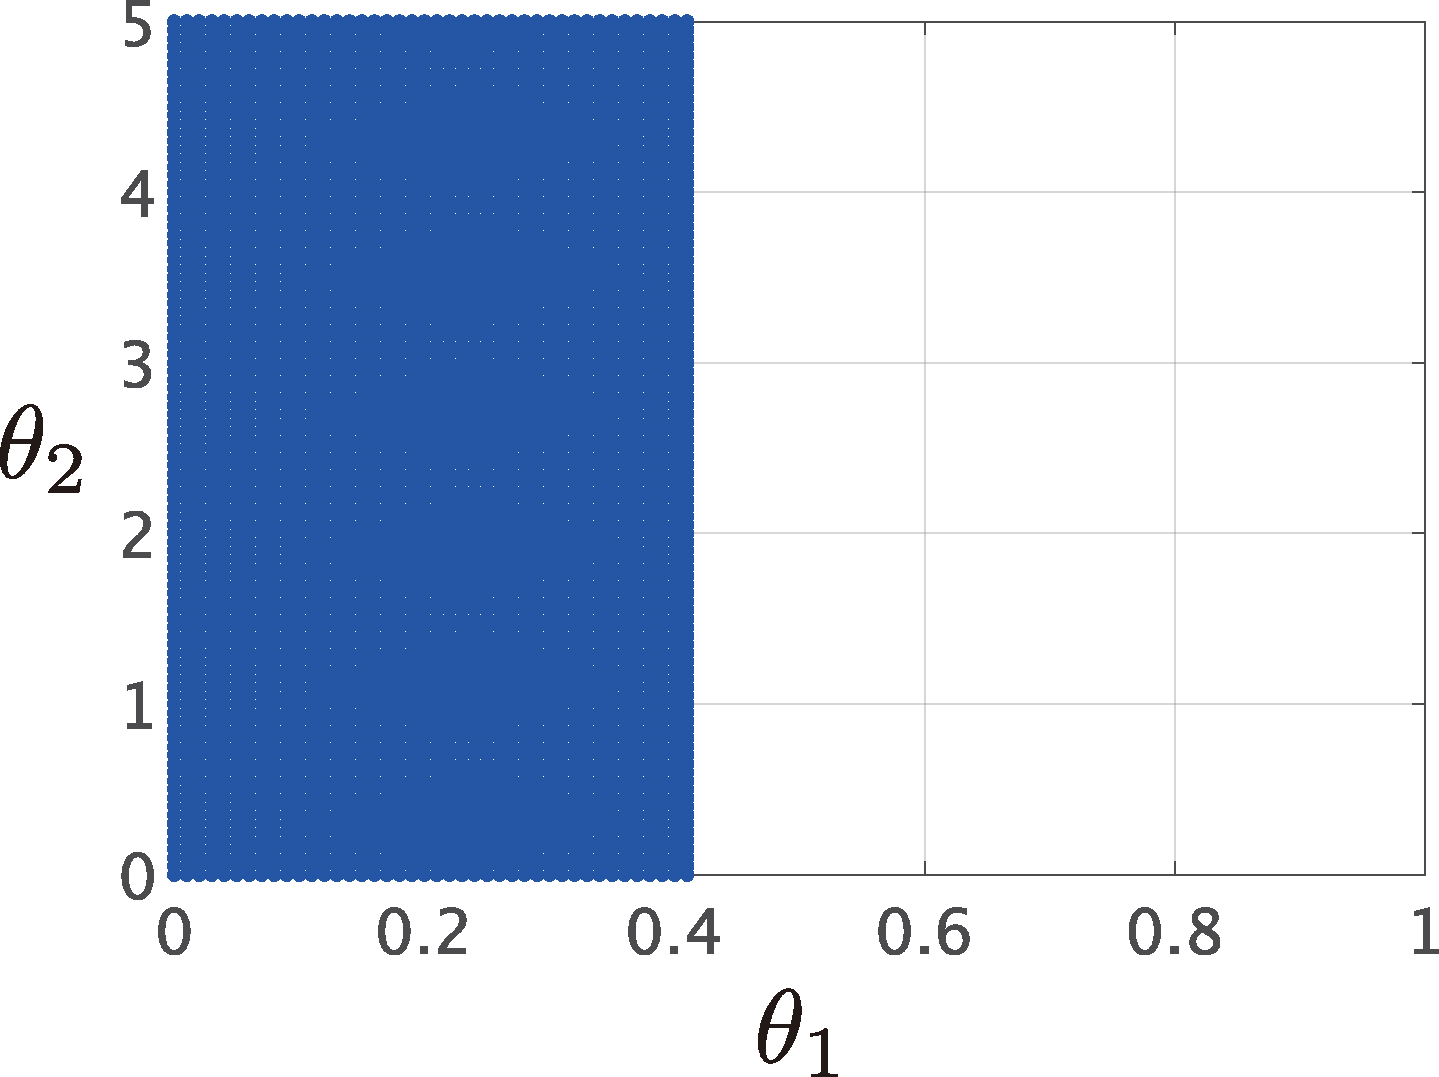
\includegraphics[width = 0.90\linewidth]{figs/Y1D1}
    \subcaption{ $D=(10,10,10)$,$\bm{Y}=\bm{Y}_0$ }
    \medskip
  \end{minipage}
  \begin{minipage}{0.49\linewidth}
    \centering
    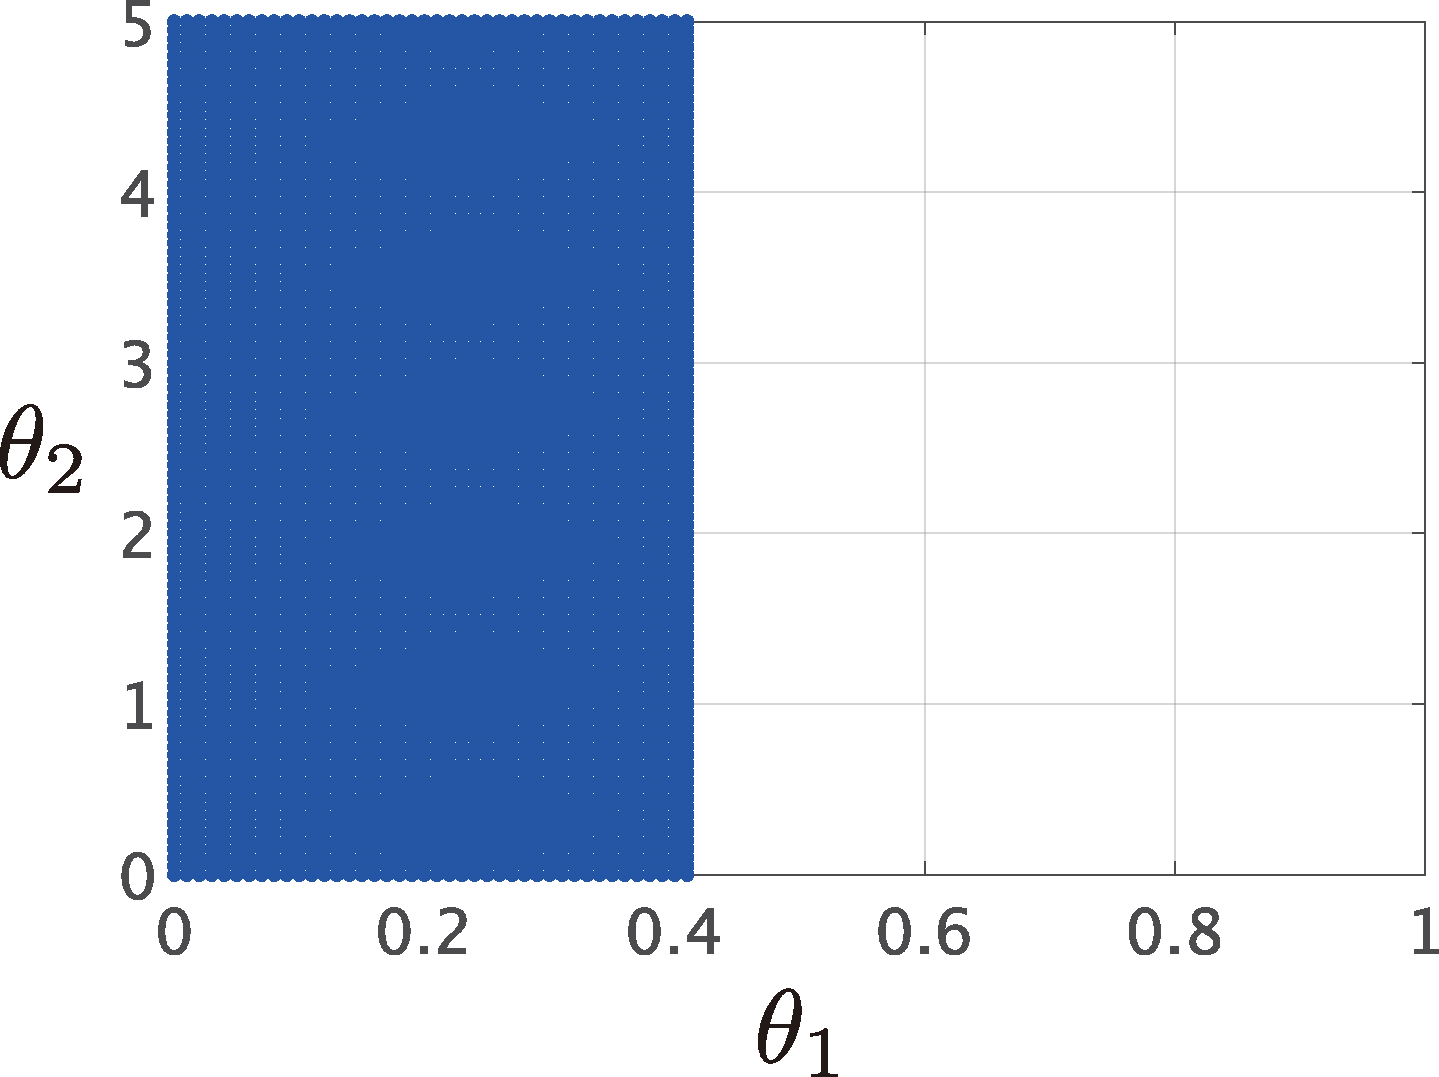
\includegraphics[width = 0.90\linewidth]{figs/Y1D0.01}
    \subcaption{$D=(\tfrac{1}{10}\tfrac{1}{10},\tfrac{1}{10})$,$\bm{Y}=\bm{Y}_0$ }
    \medskip
  \end{minipage}
}
  \centering
  {
  \begin{minipage}{0.49\linewidth}
      \centering
    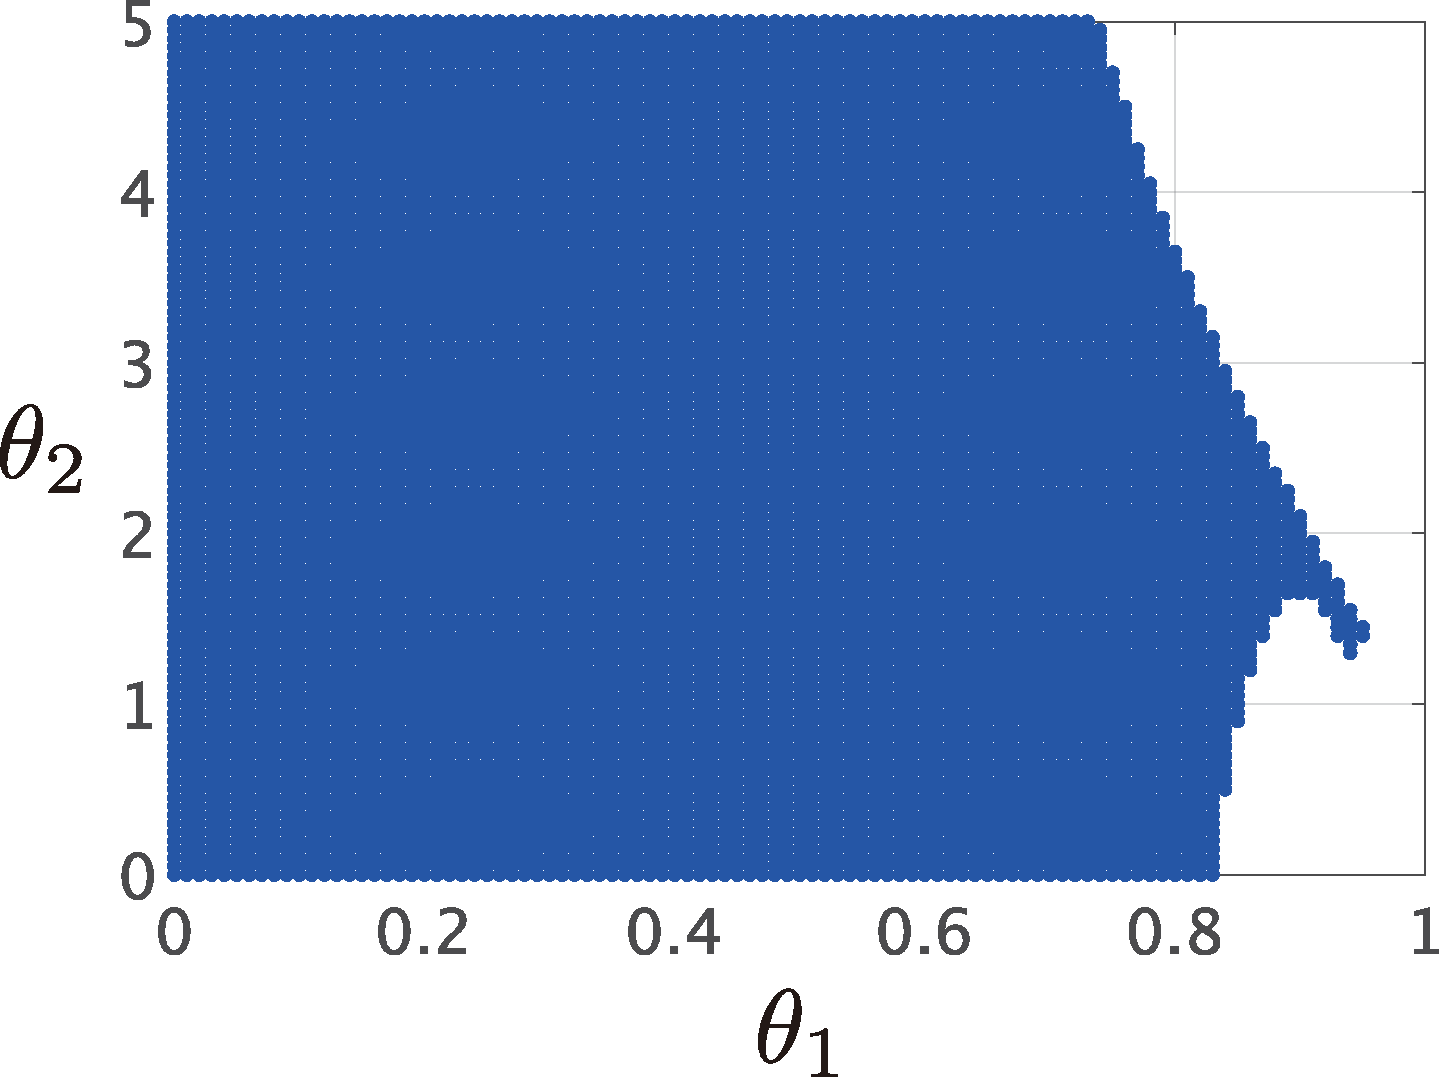
\includegraphics[width = 0.90\linewidth]{figs/Y0.01D1}
    \subcaption{$D=(10,10,10)$, $\bm{Y}=\tfrac{\bm{Y}_0}{100}$ }
    \medskip
  \end{minipage}
  \begin{minipage}{0.49\linewidth}
    \centering
    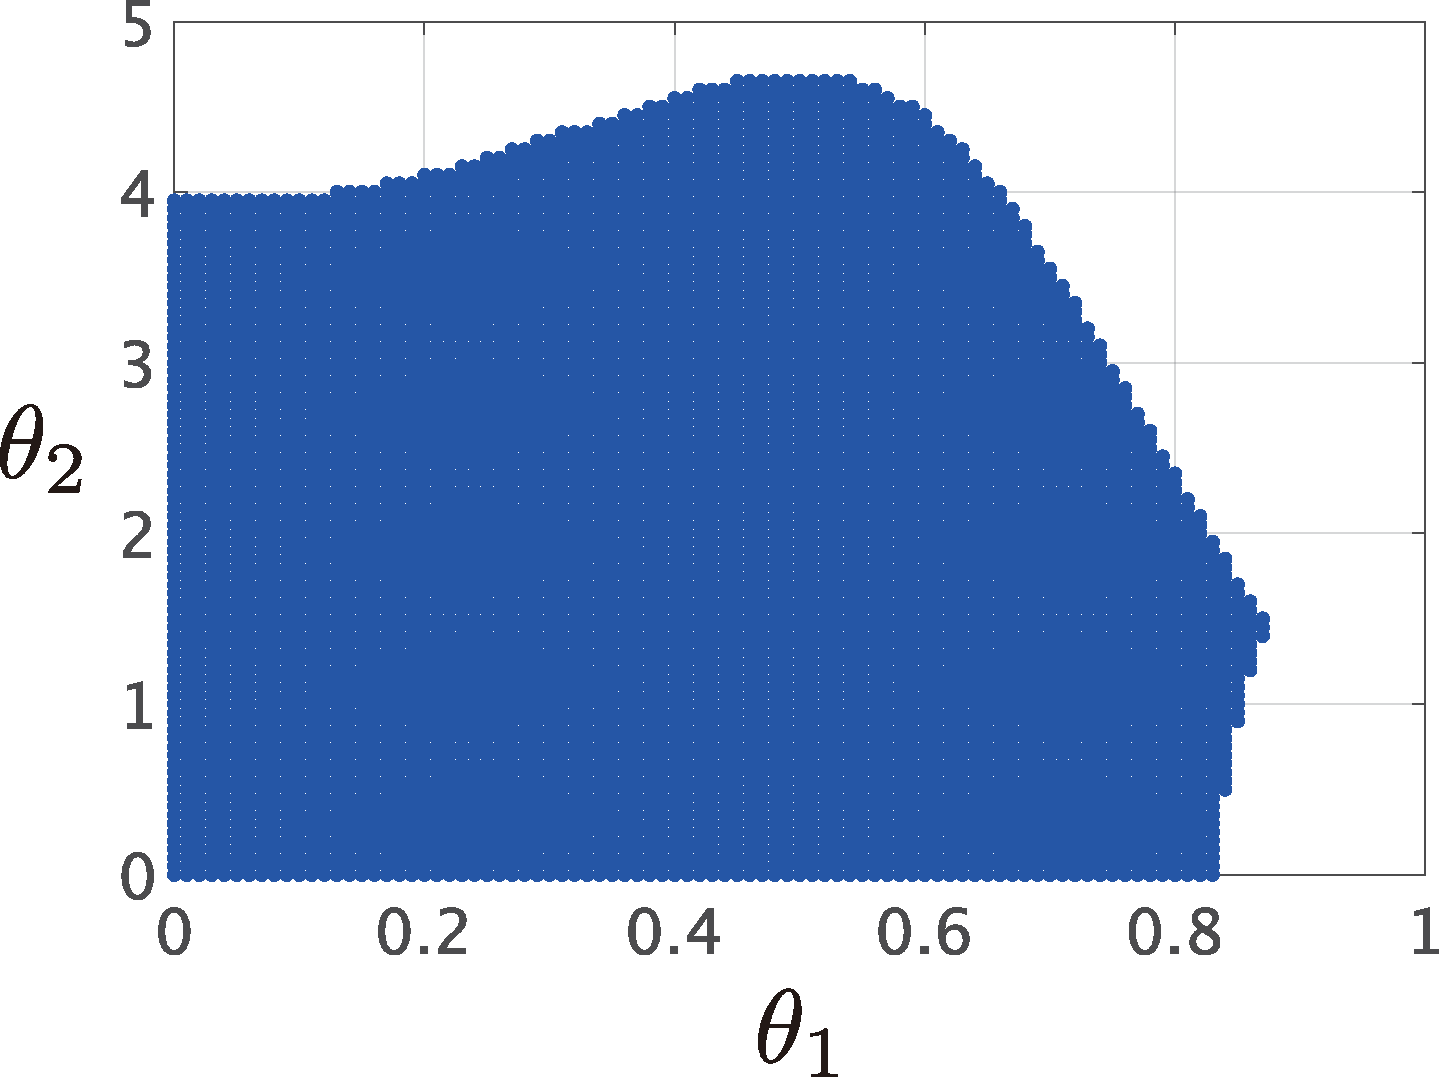
\includegraphics[width = 0.90\linewidth]{figs/Y0.01D0.01}
    \subcaption{$D=(\tfrac{1}{10},\tfrac{1}{10},\tfrac{1}{10})$, $\bm{Y}=\tfrac{\bm{Y}_0}{100}$}
    \medskip
  \end{minipage}
}
% \medskip
 \caption{\textbf{Area of parameters where the approximate linear model is stable}}
 \label{fig:stacheck}
\medskip
\end{figure}


\section{Mathematical stability analysis of the linearized
model\advanced}\label{sec:linmathana}

\subsection{Small signal stability of the linearized model\advanced}
In this section, we mathematically analyze the stability of the linearized model
given in equation \ref{eq:lindynu0}. The stability is characterized by the
eigenvalues of the matrix $\Psi$. However, as discussed in section
\ref{sec:numlinsta}, $\Psi$ is not regular and the eigenspace for the zero
eigenvalue is given by

\begin{equation}\label{eq:eqset}
  \mathcal{M} =
  \sfspan\left\{
  \mat{
  \mathds{1}\\
  0\\
  0
  }
  \right\}
\end{equation}
%\footnote{
%正方行列$A$のある固有値$\lambda$に対して
%\[
%\mathcal{V}_{\lambda}:= \sfker (\lambda I -A)
%\]
%を$\lambda$に対する\emph{固有空間}(eigenspace)と呼ぶ。
%固有値$\lambda$に対するすべての線形独立な固有ベクトルを$v_1,\ldots,v_k$とするとき
%\[
%\mathcal{V}_{\lambda} = \sfspan\{v_1,\ldots,v_k\}
%\]
%が成り立つ。
%すなわち,特定の固有値に対する固有ベクトルが張る線形空間である。
%}
%。
This eigenspace represents the set of equivalent steady-state values obtained by
varying the phase angles of all generators while maintaining their relative
values constant. Therefore, it is not a problem which point in the equilibrium
set of Equation \ref{eq:eqset} the state of the approximate linear model
converges to. Based on this fact, we give the following definition:

\begin{COLUMN}
\noindent \textbf{Eigenspace of a square matrix}:
For a square matrix $A$ and a given eigenvalue $\lambda$, the \emph{eigenspace}
\index{eigenspace} $\mathcal{V}_{\lambda}$ is defined as:

\[
  \mathcal{V}_{\lambda}:= \sfker (\lambda I -A)
\]
where $\sfker$ denotes the kernel of the matrix. If $v_1,\ldots,v_k$ are all
linearly independent eigenvectors corresponding to a specific eigenvalue
$\lambda$, then:

\[
\mathcal{V}_{\lambda} = \sfspan\{v_1,\ldots,v_k\}
\]
which means that it is a linear space spanned by the eigenvectors associated
with a specific eigenvalue.

\end{COLUMN}


\begin{definition}[Small-signal stability of the linear approximation model]
\label{def:stalin}

Consider the linearized model given by Equation \ref{eq:lindynu0}. For any
initial values, if the internal state converges to one of the equilibrium points
in the set $\mathcal{M}$ defined by Equation \ref{eq:eqset}, the linearized
model is said to be \textbf{steady-state stable}\index{steady-state stability}.
%\footnote{
%電力系統工学では,微小な外乱に対する電力系統の安定性を近似線形モデルを用いて議論する場合に広く「定態安定性」という用語が用いられる。
%ただし,definition\ref{def:stalin}のように数学的なdefinitionを導入することは一般的ではない。
%}。
\end{definition}
The small-signal stability in Definition \ref{def:stalin} means that for any
initial condition, Equation \ref{eq:linmconv} holds. Note that the value of
$c_0$ in Equation \ref{eq:linmconv} is arbitrary, so we express its
arbitrariness as "converging to one of the equilibrium points in $\mathcal{M}$."

In power system engineering, the term "small-signal stability" is widely used to
discuss the stability of a power system against small disturbances using an
approximate linear model. However, introducing a mathematical definition like
Definition \ref{def:stalin} is not common practice.

In the following discussion, we assume that the kernel space of $\Psi$ in
Equation \ref{eq:lindynu0} is one-dimensional and that Equation
\ref{eq:nesconker} holds:
\begin{equation}\label{eq:nesconker}
  \sfker \Psi = \mathcal{M}
\end{equation}
It is clear from the structure of the matrix $\Psi$ that $\mathcal{M}$ is a
subset of $\sfker \Psi$, but it should be noted that we are assuming that
$\sfker \Psi$ is one-dimensional and that the equality holds. If the kernel
space were two-dimensional or greater, the invariant eigenspace would be larger
than $\mathcal{M}$, and the approximate linear model would not be in a steady
state stability.
%\footnote{
%行列$\Psi$の構造から,$\mathcal{M} \subseteq \sfker \Psi $であることは明らかであるが,ここでは$\sfker \Psi$が1次元であり,等号が成り立つことを仮定している。
%この核空間が2次元以上であると,不変な固有空間が$\mathcal{M}$よりも大きくなり,近似線形モデルは定態安定とならない。
%}
%。
Therefore, equation \ref{eq:nesconker} is a necessary condition for the
steady-state stability of the linear approximation model. In particular, when
$A$ is invertible, and using the definition of $L_0:= L-CA^{-1}B$, the
necessary condition can be equivalently expressed as:
\begin{equation}\label{eq:nescon}
  \sfker L_0 = \sfspan
  \left\{
  \mathds{1}
  \right\}
\end{equation}
Note that this matrix $L_0$ plays an important role in the subsequent analysis.

The relationship between equation \ref{eq:defL0} and equation \ref{eq:nescon}
can be verified as follows. Because the $(1,2)$ block of the matrix $\Psi$ is
invertible, the necessary and sufficient condition for the kernel of $\Psi$ to
be equal to $\mathcal{M}$ is:

\begin{equation*}%\label{eq:nescon0}
  \sfker \mat{
  -L & -C \\
  B & A
  }
  = \sfspan
  \left\{
  \mat{
  \mathds{1}\\
  0
  }
  \right\}
\end{equation*}

In particular, when $A$ is invertible, we have
\begin{align*}
\mat{
-L & -C \\
B & A
}\mat{x\\y}
=0
\qquad
\Longleftrightarrow
\quad
L_0 x=0,
\qquad
y=-A^{-1}Bx
\end{align*}
Thus, the necessary condition is equivalent to equation \ref{eq:nescon}.

For the following discussion, we introduce the following fundamental
terminology.

\begin{definition}[Stability of square matrix]
\label{def:matsta}
For a square matrix $A$, if all the real parts of its eigenvalues are negative,
$A$ is called \textbf{stable}\index{stable} or \textbf{asymptotically
stable}\index{asymptotically stable}.
\end{definition}

\subsection{Passivity of approximate linear models\advanced}\label{sec:linpasana}

\smallskip
\subsubsection{Representation of Approximate Linear Models with Feedback}

\begin{figure}[t]
\centering
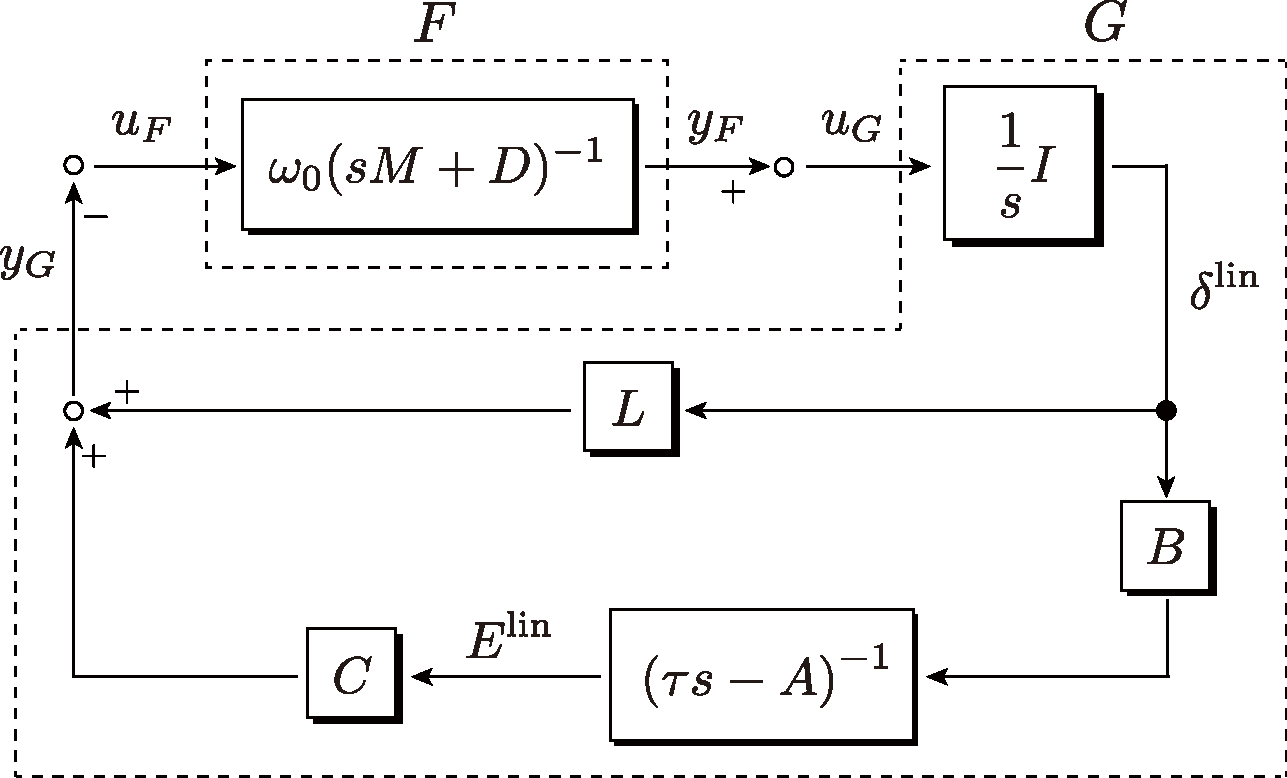
\includegraphics[width = .7\linewidth]{figs/FandG}
\medskip
\caption{\textbf{Feedback system representation of approximate linear models}}
\label{fig:GandG}
\medskip
\end{figure}

Let us consider describing the approximate linear model of Equation
\ref{eq:lindynu0} as a feedback system of two subsystems (Figure
\ref{fig:GandG}).  The first subsystem is described as a system of differential
equations for the deviation of the angular frequency:

\begin{equation}\label{eq:Fss}
  F: \simode{
  M \Delta \dot{\omega}^{\rm lin} &= -D \Delta \omega^{\rm lin}
  +
  u_F \\
  y_F &= \omega_0 \Delta \omega^{\rm lin}
  }
\end{equation}

In this book, we refer to this subsystem as the \textbf{mechanical
subsystem}\index{mechanical subsystem}. The mechanical subsystem is determined
solely by the physical constants of the generator set $(M_i, D_i){i \in
\mathcal{I}\text{G}}$ and the reference angular frequency $\omega_0$, and does
not depend on the steady-state values of the internal state $(\delta^{\star},
E^{\star})$.

The second subsystem is described as a system of differential equations with
respect to the rotor angle and internal voltage as follows:
\begin{equation}\label{eq:Gss}
  G: \simode{
  \dot{\delta}^{\rm lin} & = u_G \\
  \taud \dot{E}^{\rm lin} &= A E^{\rm lin} + B \delta^{\rm lin} \\
  y_G &= C E^{\rm lin} + L \delta^{\rm lin}
  }
\end{equation}

We call this subsystem the \textbf{electrical subsystem}\index{Electrical
subsystem} \footnote{The terms "mechanical subsystem" and "electrical subsystem"
introduced here are unique to this book.}.  The electrical subsystem not only
depends on the physical constants of the generator group, $(\taudi){i\in
\mathcal{I}{\rm G}}$, but also on the steady-state values of the internal
states, $(\delta^{\star},E^{\star})$. In fact, the system matrix $(L,A,B,C)$ in
equation \ref{eq:sysmats} is a function of $(\delta^{\star},E^{\star})$.

If the two subsystems' inputs and outputs are coupled through negative feedback
as follows:
\begin{align}\label{eq:nfedcon}
  u_F = -y_G,\qquad
  u_G = y_F
\end{align}
the approximate linear model of Equation \ref{eq:lindynu0} is represented. The
subsequent analysis of steady-state stability is based on the property called
the \textit{passivity} of the mechanical and electrical subsystems. It is
well-known that a negative feedback system of a passive subsystem is stable.

\smallskip
\subsubsection{Passivity of the mechanical subsystem}

The mechanical subsystem $F$ in Equation \ref{eq:Fss} has the following strong
passivity:

\begin{definition}[Passivity of linear systems]\label{def:passivelin}

Consider the linear system
\begin{equation}\label{eq:siglin}
  \Sigma: \simode{
  \dot{x} &= Ax + Bu \\
  y &= Cx 
  }
\end{equation}

Using the symmetric matrix $P$, define the function:
\begin{equation}\label{eq:defstlin}
  W(x):= \frac{1}{2}x^{\sf T}Px
\end{equation}

For any $u$, if there exists a semi-positive definite matrix $P$ that satisfies:
\begin{align}\label{eq:conpvlin}
\frac{d}{dt} W\bigl( x(t) \bigr) \leq u^{\sf T}(t) y(t)
,\qquad
\forall t \geq 0
\end{align}
Then, we call $\Sigma$ \textbf{passive}\index{passive}.

In particular, when there exists a positive definite number $\rho$ such that in
addition to the semi-positive definite matrix, the inequality:
\begin{align}\label{eq:conosplin}
\frac{d}{dt} W\bigl( x(t) \bigr) \leq u^{\sf T}(t) y(t) -\rho \left\|y(t) \right\|^2
,\qquad
\forall t \geq 0
\end{align}
is satisfied, then we call $\Sigma$ \textbf{strictly passive}\index{strictly
passive}.

\end{definition}

The function $W(x)$ in Definition \ref{def:passivelin} is generally called the
\textbf{storage function}\index{storage function}. Moreover, the inequality in
Equation \ref{eq:conosplin} describes a type of passivity that is more strictly
called \textbf{output-strict passivity}\index{output-strict passivity}, where
the energy represented by the storage function $W(x)$ dissipates more quickly in
proportion to the square of the output compared to the passivity in Equation
\ref{eq:conpvlin}.

The mechanical subsystem $F$ of Equation\ref{eq:Fss} having strong passivity can
be confirmed as follows. First, the subsystem is written as below:
\begin{align}
  F: \simode{
  \dot{x}_F & = A_F x_F + B_F u_F \\
  y_F &= C_F x_F
  }
\end{align}
where state $x_F$ represents $\Delta \omega^{\rm lin}$, and the system matrices
are:
\[
  A_F := -M^{-1}D,\qquad
  B_F := M^{-1},\qquad
  C_F := \omega_0 I
\]

Additionally, we define the symmetric matrix $P_F$ as:
\[
  P_F := \omega_0 M
\]
and since $M$ is positive definite, $P_F$ is also positive definite.
Then, the following inequalities hold:

\[
  A^{\sf T}_F P_F + P_F A_F \preceq  
  - \frac{ 2 \sfmin \left\{ D_i \right\}}{\omega_0} C_F^{\sf T} C_F
  ,\qquad
  P_F B_F = C_F^{\sf T}
\]

Therefore, when the storage function is defined as:
\begin{align}\label{eq:WFdef}
W_F(x_F):= \frac{1}{2}x_F^{\sf T}P_Fx_F
\end{align}
the time derivative along the solution trajectory of $F$ is evaluated as:

\begin{align}\label{eq:Flyapeq}
\spliteq{
\frac{d}{dt} W_F \bigl( x_F (t) \bigr)
& = 
\nabla W_F^{\sf T}(x_F) \frac{d x_F}{dt} 
 \\
&=  \bigl( P_F x_F(t) \bigr)^{\sf T} \bigl(A_F x_F(t) + B_F u_F(t) \bigr) \\
 & = y_F^{\sf T}(t) u_F(t)
 + \frac{1}{2} x_F^{\sf T}(t) \left(A^{\sf T}_F P_F + P_F A_F\right) x_F(t) \\
& \leq 
y_F^{\sf T}(t) u_F(t)
- \tfrac{\sfmin \left\{ D_i \right\}}{\omega_0}
\|y_F(t) \|^2
}
\end{align}
where $\nabla W_F(x_F)$ is the gradient function obtained by partially
differentiating $W_F(x_F)$ with respect to its elements and arranging them
vertically. From this, it can be seen that the machine subsystem $F$ in Equation
\ref{eq:Fss} is strongly passive for any positive definite $(M_i,D_i)_{i \in
\mathcal{I}_{\rm G}}$. Note that the function $W_F(x_F)$ represents the
mechanical kinetic energy of the power system.

\smallskip
\subsubsection{Passivity of the electrical subsystem}
Next, we consider the electrical subsystem $G$ in Equation \ref{eq:Gss}. Unlike
the mechanical subsystem $F$, the electrical subsystem $G$ only possesses
passivity under limited conditions. While this may seem arbitrary, we consider
the case where all reduced conductances in Equation \ref{eq:figi} are zero, in
other words:

\begin{equation}\label{eq:Gredcon}
  G^{\rm red}_{ij}=0,\qquad 
  \forall (i, j) \in \mathcal{I}_{\rm G} \times \mathcal{I}_{\rm G}
\end{equation}

Excluding special cases, the condition in Equation \ref{eq:Gredcon} only holds
when the conductance of all transmission lines in the power system is zero, or
equivalently, the resistance of all transmission lines is zero. In this case,
for the functions $k_{ij}(\delta_{ij})$ and $h_{ij}(\delta_{ij})$ defined in
Equation \ref{eq:defkh}, the following holds: 

\begin{equation*}
  k_{ij}(\delta_{ij}^{\star}) =
  k_{ji}(\delta_{ji}^{\star})
  ,\qquad
  h_{ij}(\delta_{ij}^{\star}) = 
  - h_{ji}(\delta_{ji}^{\star}),\qquad
  h_{ii}(\delta_{ii}^{\star}) = 0
\end{equation*}

Therefore, for the system matrix $(L,A,B,C)$ in Equation \ref{eq:sysmats}, it
holds that:
\begin{equation}\label{eq:sysmatst}
  L=L^{\sf T} ,\qquad
  \hat{A} = \hat{A}^{\sf T},\qquad
  C= -\hat{B}^{\sf T}
\end{equation}
In the following, we use the symmetric structure of this special system matrix
to analyze the passivity of the electrical subsystem.

First, let us express the electrical subsystem $G$ of Equation \ref{eq:Gss} as
follows:
\begin{align}
  G: \simode{
  \dot{x}_G & = A_G x_G + B_G u_G \\
  y_G &= C_G x_G
  }
\end{align}
where the state $x_G$ is a column vector obtained by concatenating
${\delta}^{\rm lin}$ and $ E^{\rm lin} $, and $\Omega$ is a positive definite
diagonal matrix defined as follows:

\[
  \Omega :=
  \sfdiag \left( \sqrt{\frac{ \Xsi - \Xti }{ \taudi } } \right)_{i \in \mathcal{I}_{\rm G} }
\]

The system matrices are expressed as:

\[
  A_G := 
  \mat{
  0 & 0 \\
  \Omega^2 \hat{B}   &  \Omega^2 \hat{A} 
  },\qquad
  B_G := 
  \mat{
  I \\
  0
  },\qquad
  C_G := 
  \mat{
  L & -\hat{B}^{\sf T}
  }
\]

Furthermore, we define the symmetric matrix $P_G$ as follows:

\begin{equation}\label{eq:defPG}
  P_G := 
  \mat{
    L  &  - \hat{B}^{\sf T} \\
    - \hat{B} & -\hat{A}
  }
\end{equation}

The following inequalities hold for these matrices:

\begin{equation}\label{eq:lyapinG}
  A^{\sf T}_G P_G + P_G A_G \preceq 
  0
  ,\qquad
  P_G B_G = C_G^{\sf T}
\end{equation}

If we calculated the left of the inequality, it can be expressed as follows
using a symmetric matrix $\hat{A}_{\Omega} := \Omega \hat{A} \Omega$:
\[
\frac{
A^{\sf T}_G P_G + P_G A_G
}{2}
=
\mat{
\Omega \hat{B} & 0\\
0 &\Omega^{-1}
}^{\sf T}
\underbrace{
\mat{
-I & -\hat{A}_{\Omega} \\
-\hat{A}_{\Omega} & - \hat{A}_{\Omega}^2
}
}_{Y}
\mat{
\Omega \hat{B} & 0\\
0 & \Omega^{-1}
}
\]

Here, the top-left block $- I$ of $Y$ is negative definite, and the Schur
complement of $Y$ with respect to $-I$ is 0, which implies that $Y$ is negative
semi-definite. Therefore, the matrix inequality in Equation \ref{eq:lyapinG}
holds.

\begin{COLUMN}
\noindent \textbf{Schur complement}:

Let a symmetric matrix $M$ be partitioned as
\[
  M =\mat{
    M_{11} & M_{12} \\
    M_{12}^{\sf T} & M_{22}
  }
\]

Then, the \textbf{Schur complement}\index{Schur complement} of $M$ with respect
to $M_{22}$ is defined as:

\[
  M/M_{22} := M_{11} - M_{12} M_{22}^{-1} M_{12}^{\sf T}
\]

Similarly, the Schur complement of $M$ with respect to $M_{11}$ is defined as:

\[
  M/M_{11} := M_{22} - M_{12}^{\sf T} M_{11}^{-1} M_{12}
\]

If the matrix $M_{22}$ is positive definite, then $M$ is positive semidefinite
if and only if $M/M_{22}$ is positive semidefinite. The same fact holds for the
Schur complement of $M$ with respect to $M_{11}$ \cite{bernstein2009matrix}. The
same fact holds if we replace positive semidefinite with positive definite.

\smallskip
\noindent \textbf{Properties of semidefinite matrices}:

For any positive semidefinite (or negative semidefinite) matrix $Y\in
\mathbb{R}^{n\times n}$ and any matrix $X\in \mathbb{R}^{n\times m}$, the matrix
$X^{\sf T}YX$ is positive semidefinite (or negative semidefinite). This can be
shown from the fact that

\[
  v^{\sf T}Yv\geq 0, \quad \forall v\in \mathbb{R}^n
  \qquad
  \Longrightarrow
  \qquad
  (Xw)^{\sf T} Y (Xw) \geq 0, \quad \forall w\in \mathbb{R}^m
\]
\end{COLUMN}

By using the relationship given by Equation \ref{eq:lyapinG}, the time
derivative of the storage function $W_G(x_G)$ along the solution trajectory of
$G$ can be evaluated, where $W_G(x_G)$ is defined by Equation \ref{eq:WGdef},
similarly to Equation \ref{eq:Flyapeq}:

\begin{equation}\label{eq:WGdef}
  W_G(x_G):= \frac{1}{2}x_G^{\sf T}P_Gx_G
\end{equation}

\begin{align}\label{eq:Glyapeq}
\frac{d}{dt} W_G \bigl( x_G (t) \bigr)
 \leq 
y_G^{\sf T}(t) u_G(t)
\end{align}

However, to show the passivity of $G$, $P_G$ in equation \ref{eq:defPG} must be
positive semi-definite. If the matrix $A$ in equation \ref{eq:sysmats} is
stable, then it can be shown that:

\[
  A= S^2 \hat{A}
  \qquad \Longleftrightarrow \qquad S^{-1} A S = S \hat{A} S
\]
where $S:=\sfdiag \left( \sqrt{ \Xsi - \Xti }\right){i \in \mathcal{I}{\rm G} }$.
Here, $\hat{A}$ is negative definite. Under this condition, the necessary and
sufficient condition for $P_G$ in Equation \ref{eq:defPG} to be positive
semi-definite is that the Schur complement of $-\hat{A}$ is positive
semi-definite, in other words:

\begin{align}\label{eq:pdsp}
L_0 =L_0^{\sf T} \succeq 0
\end{align}
where $L_0$ is defined by Equation \ref{eq:defL0} and can be expressed as $L_0 =
L + \hat{B}^{\sf T} \hat{A}^{-1} \hat{B}$ using Equation \ref{eq:sysmatst}. To
summarize the above discussion, the following definition is introduced.

\begin{definition}[Passive power transmission condition]\label{def:passtrans}
For the system matrix $(L,A,B,C)$ of Equation \ref{eq:sysmats}, the following
three conditions are together called \textbf{passive power transmission
conditions}.
\footnote{
"Passive power transmission conditions" is a term unique to this book.
}
\begin{itemize}
  \item[(i)] Matrix $A$ is stable.
  \item[(ii)] As in Equation \ref{eq:Gredcon}, all reduced conductances are zero. 
  \item[(iii)] For the matrix $L_0$ of Equation \ref{eq:defL0}, the matrix inequality of Equation \ref{eq:pdsp} holds. 
\end{itemize}

Each of these conditions may be referred to individually as the passive
transmission condition (i), and so on.
\end{definition}

Based on the above discussions, we can see that the passive power transmission
conditions describe the conditions necessary for the electrical system $G$ of
Equation \ref{eq:Gss} to be passive. Furthermore, these conditions are necessary
for the linear approximation model to be statically stable for the passivity of
an electrical subsystem and arbitrary physical constant. The details are
discussed in Section \ref{sec:nesconana} and Section \ref{sec:nesconsta}.
Function $W_G(x_G)$ indicates the electrical potential energy of an electrical
power system.

\subsection{Analysis of small signal stability based on passivity\advanced}

\smallskip
\subsubsection{Stability analysis of feedback systems}

In the following, under the passive power transmission conditions defined in
Definition \ref{def:passtrans}, the small signal stability of the linear
approximation model given in Equation \ref{eq:lindynu0} is analyzed for electric
subsystems that are passive. The stability of their feedback systems is also
analyzed.

Since the inequalities in Equations \ref{eq:Flyapeq} and \ref{eq:Glyapeq} hold,
their sum is given by:

\smallskip
\begin{equation*}
  \begin{aligned}
    \spliteq{
      \frac{d}{dt} \bigl\{ W_F \bigl( x_F (t) \bigr)
      & +
      W_G \bigl( x_G (t) \bigr)
      \bigr\} \\
      & \leq 
      \underbrace{
      y_F^{\sf T}(t) u_F(t)
      +
      y_G^{\sf T}(t) u_G(t)
      }_{\star}
      - \tfrac{\sfmin \left\{ D_i \right\}}{\omega_0}
      \|y_F(t) \|^2
    }
  \end{aligned}
\end{equation*}

By substituting the feedback coupling equation in Equation \ref{eq:nfedcon} into
this inequality, the term indicated by "$\star$" is cancelled out, and the
inequality for the entire feedback system can be expressed as:

\begin{equation}\label{eq:FGlyapeq}
 \frac{d}{dt} \bigl\{ W_F \bigl( x_F (t) \bigr)
 +
 W_G \bigl( x_G (t) \bigr)
 \bigr\} 
 \leq 
- \tfrac{\sfmin \left\{ D_i \right\}}{\omega_0}
\|y_F(t) \|^2
\end{equation}

In other words, the sum of the functions $W_F(x_F)$ and $W_G(x_G)$ is
monotonically non-increasing with respect to the time evolution along the
feedback system trajectory. Furthermore, since the lower bounds of $W_F(x_F)$
and $W_G(x_G)$ are both 0, their sum asymptotically converges to a certain value
as time passes sufficiently. This means that the value of the time derivative on
the left-hand side of Equation \ref{eq:FGlyapeq} converges to 0. Additionally,
since the right-hand side of Equation \ref{eq:FGlyapeq} is negative when $y_F(t)
\neq 0$ and is only 0 when $y_F(t) = 0$, the following is obtained: 

\begin{equation}\label{eq:yFlim0}
  \lim_{t\rightarrow \infty} y_F(t)  =0
\end{equation}

Furthermore, focusing on the output equation of Equation \ref{eq:Fss}, since the
output $y_F$ is a constant multiple of the internal state $\Delta \omega^{\rm
lin}$, it can be understood that for the mechanical subsystem $F$:

\begin{equation}\label{eq:Fobs}
  y_F(t)  =0,\quad \forall t\geq 0 
  \qquad \Longrightarrow \qquad
  \Delta \omega^{\rm lin}(t)  =0,\quad \forall t\geq 0 
\end{equation}

This is a property called \textbf{observability} in system control engineering.
Therefore, from Equations \ref{eq:yFlim0} and \ref{eq:Fobs}, for the
approximated linear model of Equation \ref{eq:lindynu0}, for any initial value
$(\Delta \omega^{\rm lin}(0),\delta^{\rm lin}(0),E^{\rm lin}(0))$, the following
holds:

\begin{equation}\label{eq:Delom0}
  \lim_{t\rightarrow \infty} \Delta \omega^{\rm lin}(t)  =0
\end{equation}

In other words, the internal state of the mechanical subsystem $F$ in Equation
\ref{eq:Fss} in the feedback system converges to 0 asymptotically.

\begin{COLUMN}
\noindent \textbf{Observability}:
For a linear system $\Sigma$ described by Equation \ref{eq:siglin}, if the
output $y(t)$ is identically zero, then the internal state $x(t)$ is also
identically zero, and $\Sigma$ is said to be \textbf{observable}
\index{observability} in this case. The necessary and sufficient condition for
$\Sigma$ to be observable is given by Equation \ref{eq:condobs}, where $n$ is
the dimension of the state.

\begin{align}\label{eq:condobs}
  \sfker \mat{
  C \\
  CA \\
  \vdots \\
  CA^{n-1}
  }
  =\{0\}
\end{align}

In some contexts, a pair of matrices that satisfies Equation \ref{eq:condobs} is
referred to as an observable pair $(C,A)$.

\smallskip
\noindent \textbf{Controllability}:
For a linear system $\Sigma$ described by Equation \ref{eq:siglin}, if there
exists an input $u(t)$ such that for all initial states $x(0)$, there exists a
time $T>0$ such that $x(T) = 0$, then $\Sigma$ is said to be
\textbf{controllable} \index{controllability}. The necessary and sufficient
condition for $\Sigma$ to be controllable is given by Equation \ref{eq:condcon},
where $n$ is the dimension of the state.

\begin{align}\label{eq:condcon}
\sfim \mat{
B & AB & \cdots &A^{n-1}B
}
= \mathbb{R}^n
\end{align}

Here, $\sfim$ denotes the \textbf{image} \index{image} of the matrix. In some
contexts, a pair of matrices that satisfies Equation \ref{eq:condcon} is
referred to as a controllable pair $(A,B)$

\smallskip
\noindent \textbf{Lyapunov function}:
Consider the observable linear system $\Sigma$ described by Equation
\ref{eq:siglin}, where the input $u(t)$ is identically zero. Let $V(x)$ be a
positive semi-definite function that satisfies $V(x)\geq 0$ for all $x$ and
$V(0)=0$. If there exists a positive constant $\rho$ such that the derivative of
$V(x)$ along the solution trajectory of $\Sigma$ satisfies

\[
  \frac{d}{dt} V \bigl( x (t) \bigr) 
  =
  \nabla V^{\sf T}(x) \frac{d x}{dt} (t)
  \leq  - \rho \|y(t)\|^2,\qquad
  \forall t \geq0
\]
then the solution trajectory $x(t)$ converges asymptotically to zero for any initial state.
Such a function $V(x)$ is called a \textbf{Lyapunov function} \index{Lyapunov function}.

\begin{figure}[h]
  \centering
  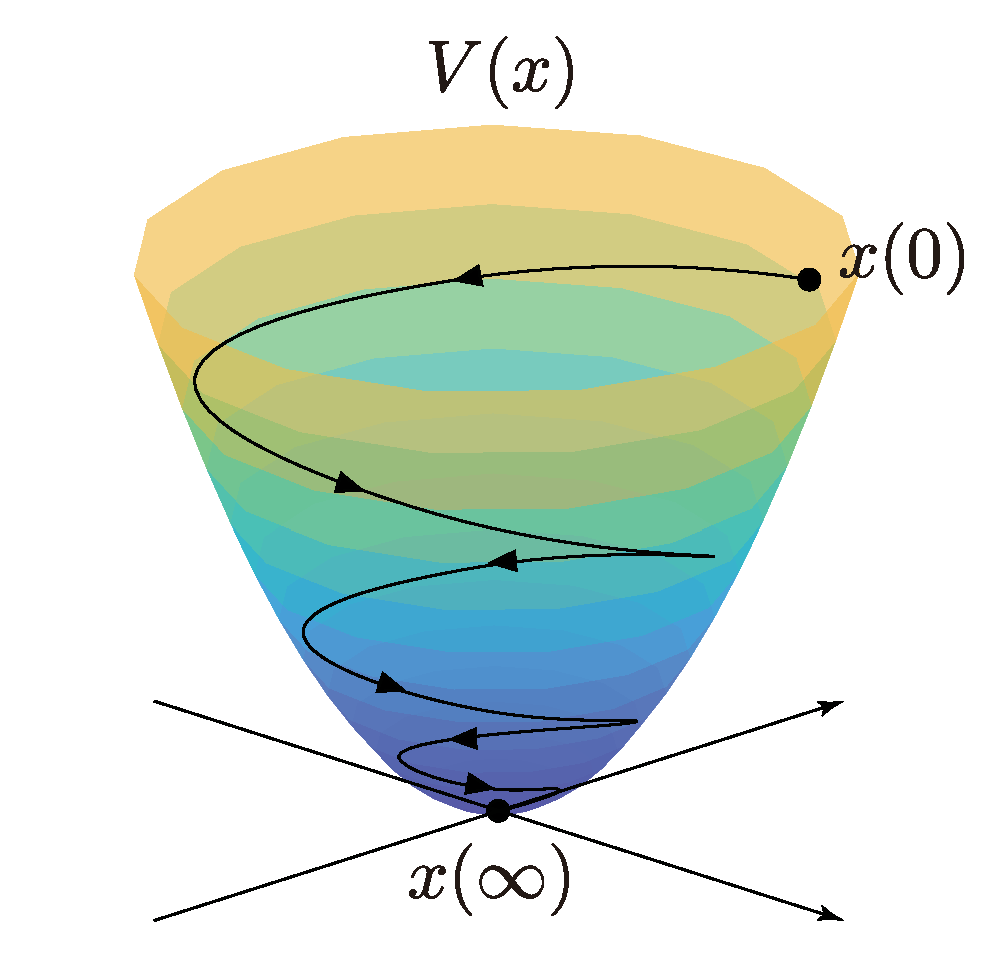
\includegraphics[width = .35\linewidth]{figs/cone}
  \caption{\textbf{Monotonically decreasing values along the solution trajectory of the Lyapunov function}}
  \label{fig:conelyap}
  \medskip
\end{figure}

The fact that the value of the Lyapunov function decreases monotonically along
the solution trajectory of the system can be interpreted as a type of energy
dissipation over time (Figure \ref{fig:conelyap}). Similar stability analyses
based on Lyapunov functions can also be applied to nonlinear systems.

\end{COLUMN}

On the one hand, it is not possible to deduce from the above discussion whether
the internal state of the electric subsystem $G$ in Equation \ref{eq:Gss}
converges asymptotically to 0.  Specifically, from the relation in Equation
\ref{eq:nfedcon} and the asymptotic convergence in Equation \ref{eq:Delom0}, it
can be derived that the input and output of the two subsystems satisfy:

\[
  \lim_{t\rightarrow \infty} u_F(t)  =0,\qquad
  \lim_{t\rightarrow \infty} u_G(t)  =0,\qquad
  \lim_{t\rightarrow \infty} y_G(t)  =0
\]

However, since the electric subsystem is not observable, it cannot be concluded
that its internal state converges asymptotically to zero.  Assuming that the
electric subsystem is observable, it can be concluded that for any initial
values:

\[
  \lim_{t\rightarrow \infty}  \delta^{\rm lin}(t)  =0,\qquad
  \lim_{t\rightarrow \infty}  E^{\rm lin}(t)  =0
\]

However, this implies that $c_0$ must always be equal to 0 in Equation
\ref{eq:linmconv}. This fact contradicts the instability of Equation
\ref{eq:lindynu0} due to the zero eigenvalue of $\Psi$. It should be noted that
except for some special cases, the electric subsystem is controllable.


\begin{figure}[t]
  \centering
  {
  \begin{minipage}{0.49\linewidth}
    \centering
    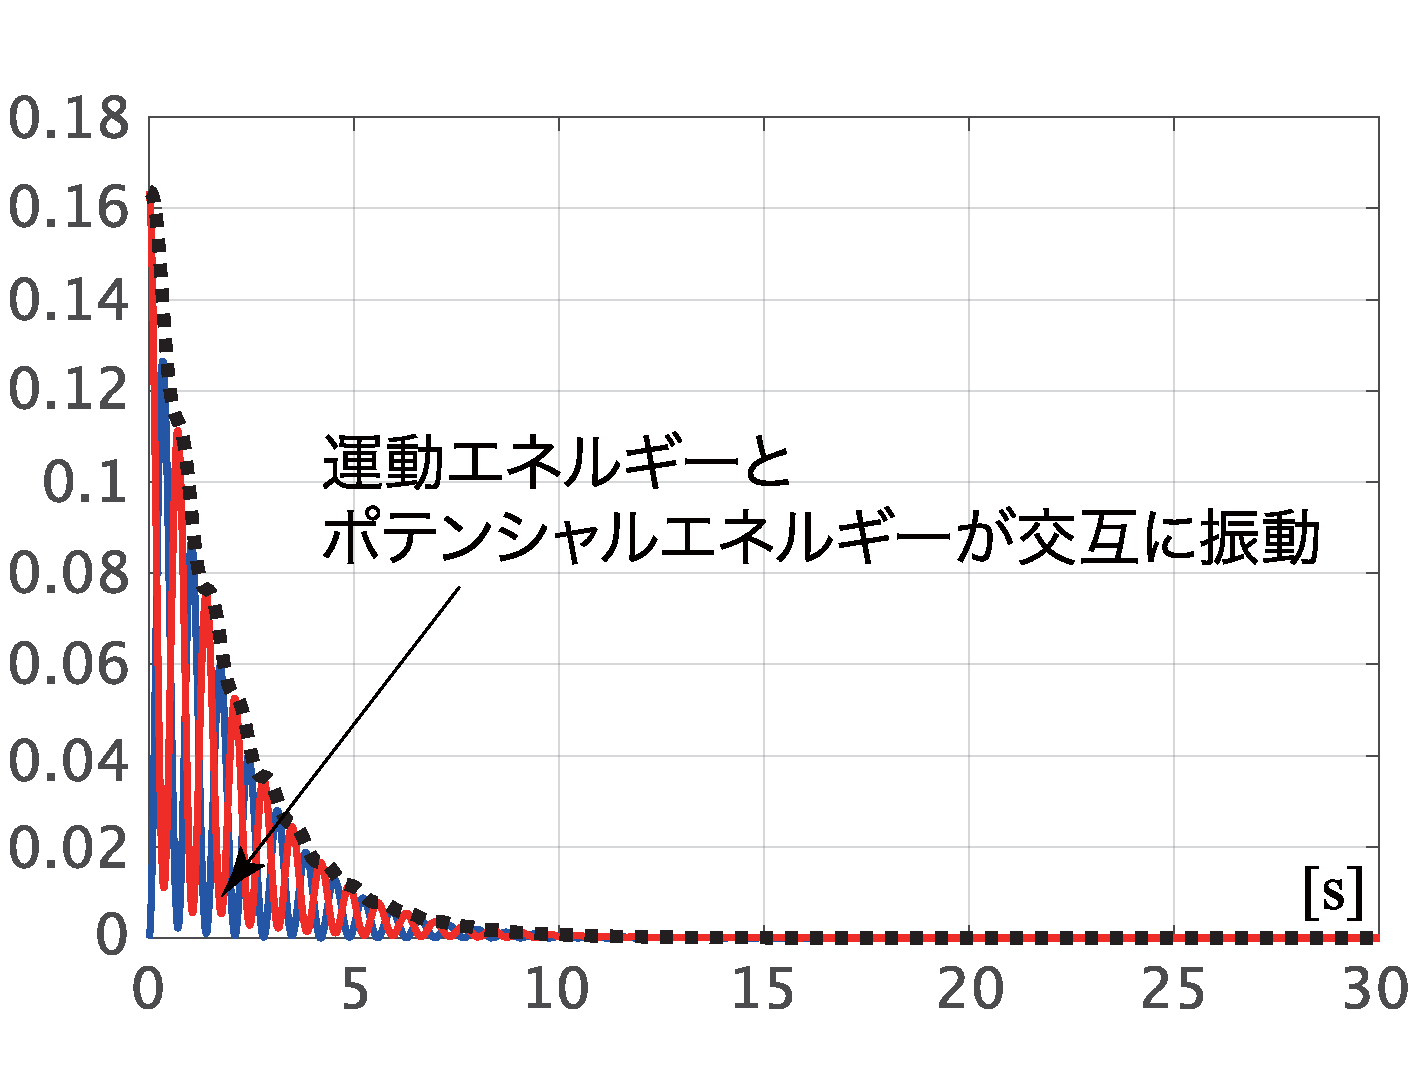
\includegraphics[width = 1.0\linewidth]{figs/losslessW}
    \subcaption{If passive transmission condition (ii) is met}
    \medskip
  \end{minipage}
  \begin{minipage}{0.49\linewidth}
    \centering
    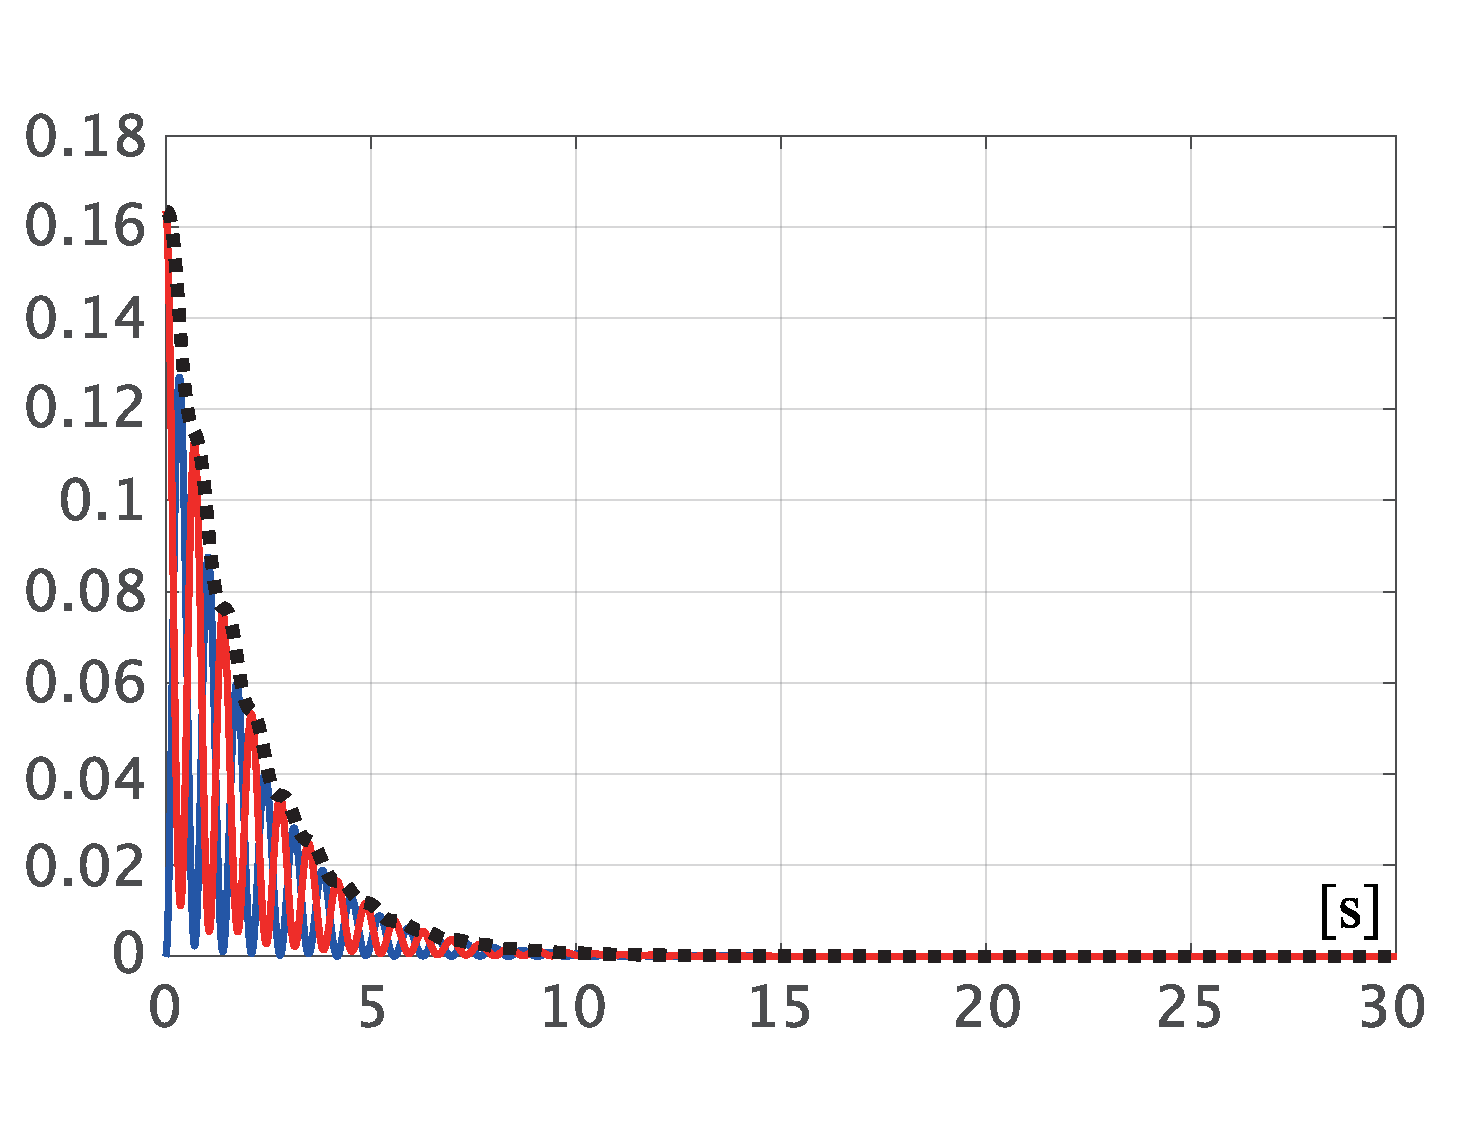
\includegraphics[width = 1.0\linewidth]{figs/lossyW}
    \subcaption{If passive transmission condition (ii) is not met}
    \medskip
  \end{minipage}
  }
  \medskip
  \caption{\textbf{Time variation of the accumulation function according to Example \ref{ex:linsyssim}}
  \\  \centering(Blue: $W_F$, Red: $W_G$, Black:$W_F+W_G$)}
  \label{fig:LyapW}
\medskip
\end{figure}


\begin{example}{Time evolution of stored energy}\label{ex:energylin}
Consider the approximated linear model discussed in the first half of Example
\ref{ex:linsyssim}. First, consider the case where the passive transmission
condition (ii) is satisfied, i.e., when the conductance of both transmission
lines is 0. Specifically, set the admittance values of the transmission lines
to:

\begin{equation}\label{eq:bothlossless}
  \bm{y}_{12} = - \bm{j} 11.6041, \qquad
  \bm{y}_{23} =  - \bm{j} 10.5107
\end{equation}

This corresponds to setting the parameter $\theta_2$ to 0 in Equation
\ref{eq:Y0theta2}. In this case, the matrix $A$ becomes stable. Also, all the
eigenvalues of $L_0$ in Equation \ref{eq:defL0} become non-negative. Thus, the
passive transmission conditions (i) and (iii) hold.

Consider the time response of the initial values in Equation \ref{eq:linmini}
and calculate the time variation of the kinetic energy $W_F(x_F)$ in Equation
\ref{eq:WFdef} and the potential energy $W_G(x_G)$ in Equation \ref{eq:WGdef}.
The calculation results are shown in Figure \ref{fig:LyapW}(a) where the blue
and red solid lines represent $W_F(x_F)$ and $W_G(x_G)$, respectively, and the
black dashed line represents their sum, which is the total energy of the system.
From this figure, it can be seen that while the kinetic and potential energies
increase and decrease alternatively, the total energy of the system, which is
the sum of these energies, decreases monotonically. The decrease in total energy
over time can be interpreted as energy loss due to friction caused by the
damping coefficient.

Next, as a reference, let us show the results when the passive power
transmission condition (ii) is not satisfied. Specifically, we set $\bm{Y}_0(1)$
in Equation \ref{eq:Y0theta2} to be the admittance matrix $\bm{Y}$ by setting
$\theta_2$ to 1. This is equivalent to calculating the time variation of the
kinetic and potential energies for the initial value response in Figure
\ref{fig:timeex}. Note that when the passive power transmission condition (ii)
is not satisfied, $P_G$ in Equation \ref{eq:defPG} does not become a symmetric
matrix, but the potential energy $W_G(x_G)$ can still be calculated using the
definition in Equation \ref{eq:WGdef}. The calculation result in Figure
\ref{fig:LyapW}(b) is almost identical to that in Figure \ref{fig:LyapW}(a).
This fact suggests that even when the conductance of the transmission line is
not zero, the electrical potential energy can be approximately calculated based
on the definition in Equation \ref{eq:WGdef}.
\end{example}

\smallskip
\subsubsection{Basis transformation for separating unobservable state variables}

Let us consider deriving an observable subsystem from the electrical subsystem
$G$ in Equation \ref{eq:Gss} by removing the common component of unobservable
rotor angles. Specifically, we apply a basis transformation to the state
$\delta^{\rm lin}$ in Equation \ref{eq:lindyn} to derive a set of differential
equations describing only the deviations of the rotor angles. Note that the
following basis transformation is always applicable regardless of whether the
passive power delivery condition holds or not.

\begin{COLUMN}
\noindent \textbf{Basis transformation of linear systems}:

In the state equation:

\[
  \dot{x}(t)=Ax(t)+Bu(t)
\]
each element $x_i(t)$ of the $n$-dimensional state vector $x(t)$ can be
represented as the component of the expansion with respect to the basis
${e_1,\ldots,e_n}$, such as:

\[
  x(t)
  =
  e_1 x_1(t) + \cdots + e_n x_n(t)
\]
where $e_i$ is an $n$-dimensional vector with only the $i$-th element being $1$.
This basis is called the \textbf{standard basis} and represents the time
evolution of the "components" of the state vector $x(t)$ in a certain basis.  We
now consider representing $x(t)$ in another basis ${v_1,\ldots,v_n}$ such that

\[
  x(t)
  =
  v_1 \xi_1(t) + \cdots + v_n \xi_n(t)
\]
where $\xi_i(t)$ is the component of the basis vector $v_i$. Let us denote the
matrix obtained by arranging the vectors $v_i$ horizontally as $V$ and the
vector obtained by arranging $\xi_i(t)$ vertically as $\xi(t)$. Then, the linear
transformation $x(t)=V\xi(t)$ corresponds to this representation. In this case,
the state equation is transformed as:

\[
  \dot{\xi}(t)=V^{-1}AV \xi(t) + V^{-1} Bu(t)
\]
where $V_{a}$ and $V_{b}$ are the matrices obtained by arranging the basis
vectors of $\mathcal{V}_a$ and $\mathcal{V}_b$ horizontally, respectively, the
transformed state equation is obtained as:

\[
  x(t)=
  V_{a} \xi_{a}(t) +
  V_{b} \xi_{b}(t)
\]
where $W_{a}$ and $W_{b}$ are matrices that satisfy:

\[
  \mat{
    \dot{\xi}_{a}(t) \\
    \dot{\xi}_{b}(t)
  }
  =
  \mat{
    W_{a} A V_{a} & W_{a} A V_{b} \\
    W_{b} A V_{a} & W_{b} A W_{b}
  }
  \mat{
    {\xi}_{a}(t) \\
    {\xi}_{b}(t)
  }
\]

However, $V_{a}$ and $V_{b}$ are matrices consisting of the basis vectors of
$\mathcal{V}a$ and $\mathcal{V}b$, respectively. $W{a}$ and $W{b}$ are matrices
that satisfy:

\[
  \mat{
    W_{a} \\
    W_{b}
  }
  =\mat{
    V_{a} & V_{b}
  }^{-1}
  \qquad
  \Longleftrightarrow
  \qquad
  \mat{
    V_{a} & V_{b}
  }\mat{
    W_{a} \\
    W_{b}
  }=I
\]

In this representation, $\xi_a(t)$ represents the component of $x(t)$ with
respect to the subspace $\sfspan \mathcal{V}_a$. Similarly, $\xi_b(t)$
represents the component of $x(t)$ with respect to the subspace $\sfspan
\mathcal{V}_b$.
\end{COLUMN}

The change of basis explained below can be applied regardless of whether passive
power transmission conditions hold. $\delta^{\rm lin}$ is expanded using a
matrix $W \in \mathbb{R}^{N\times (N-1)}$:

\begin{equation}\label{eq:batrinv}
  \delta^{\rm lin}
  =
  W
  \delta^{\rm lin}_{\rm e} +
  \mathds{1}
  \overline{\delta}^{\rm lin}_{\rm e}
\end{equation}

Here, $\mathds{1}$ is a base vector that expresses the common component of
$\delta^{\rm lin}$, while $W$ is a matrix with base vectors that express other
deviation components. In other words, the common component of $\delta^{\rm
lin}$ is $\overline{\delta}^{\rm lin}_{\rm e}$, and deviation components are
$\delta^{\rm lin}_{\rm e}$. The common component $\overline{\delta}^{\rm
lin}_{\rm e}$ is one-dimensional, while deviation components $\delta^{\rm
lin}_{\rm e}$ are $(N-1)$-dimensional.

Next, let us consider the inverse transformation of Equation \ref{eq:batrinv}.
Specifically, let us consider a matrix $W^{\dagger} \in \mathbb{R}^{(N-1)\times
N}$:
\[
  \delta^{\rm lin}
  =
  \underbrace{
  \mat{
  W & \mathds{1}
  }
  }_{T}
  \mat{
  \delta^{\rm lin}_{\rm e} \\
  \overline{\delta}^{\rm lin}_{\rm e}
  }
  \quad
  \Longleftrightarrow
  \quad
  \mat{
  \delta^{\rm lin}_{\rm e} \\
  \overline{\delta}^{\rm lin}_{\rm e}
  }
  =
  \underbrace{
  \mat{
  W^{\dagger} \\
  \frac{1}{N} \mathds{1}^{\sf T}
  }
  }_{T^{-1}}
  \delta^{\rm lin}
\]

For this inverse transformation to exist, the column vector of $W$ must be
orthogonal to $\mathds{1}$. This can be confirmed as follows. From the
relationship of inverse transformation, the following must hold:

\begin{equation*}
  T^{-1}T
  =\mat{
  W^{\dagger}W & W^{\dagger} \mathds{1}\\
  \frac{1}{N} \mathds{1}^{\sf T} W & \frac{1}{N} \mathds{1}^{\sf T} \mathds{1}
  }
  =\mat{
  I & 0\\
  0 & 1
  }
\end{equation*}

In other words, $W$ and $W^{\dagger}$ are matrices that satisfy:

\[
  \mathds{1}^{\sf T} W=0,\qquad
  W^{\dagger}W=I,\qquad
  W^{\dagger} \mathds{1}=0
\]

Therefore, from the first equation, we can see that the column vectors of $W$
must be orthogonal to $\mathds{1}$. Note that $W$ and $W^{\dagger}$ can be
constructed using an appropriate matrix $U\in \mathbb{R}^{N\times (N-1)}$ that
satisfies $\mathds{1}^{\sf T} U=0$ and $U^{\sf T}U$ is invertible, as follows:

\[
  W = U(U^{\sf T}U)^{-1},\qquad
  W^{\dagger}=U^{\sf T}
\]

In this case, the product $WW^{\dagger}$ can be expressed as the
\textbf{orthogonal projection matrix}\index{orthogonal projection matrix} onto
the orthogonal complement of $\sfspan{\mathds{1}}$:

\begin{equation}\label{eq:psudinv}
  WW^{\dagger} = I - \frac{1}{N} \mathds{1} \mathds{1}^{\sf T}
\end{equation}

The pseudoinverse of $W$ obtained in this way is called the
\textbf{Moore-Penrose pseudoinverse}\index{Moore-Penrose pseudoinverse}
\cite{bernstein2009matrix}.

In Figure \ref{fig:orthogonal}, the subspace $\sfspan{\mathds{1}}$ is shown by a
black arrow, and the orthogonal complement space $\sfspan{\mathds{1}}^{\perp}$
is shown as a plane perpendicular to it. When a vector $v$ is multiplied by the
orthogonal projection matrix $WW^{\dagger}$, the projection of $v$ onto
$\sfspan{\mathds{1}}^{\perp}$, which is the shadow cast by $v$ in the direction
perpendicular to $\sfspan{\mathds{1}}$, is obtained as $WW^{\dagger}v$.
Furthermore, the complementary relationship, shown below, indicates that it is
the orthogonal projection matrix onto $\sfspan{\mathds{1}}$'s orthogonal
complement, that is, $\sfspan{\mathds{1}}$.

\[
  I-WW^{\dagger}=\tfrac{1}{N}\mathds{1} \mathds{1}^{\sf T}
\]

\begin{figure}[t]
\centering
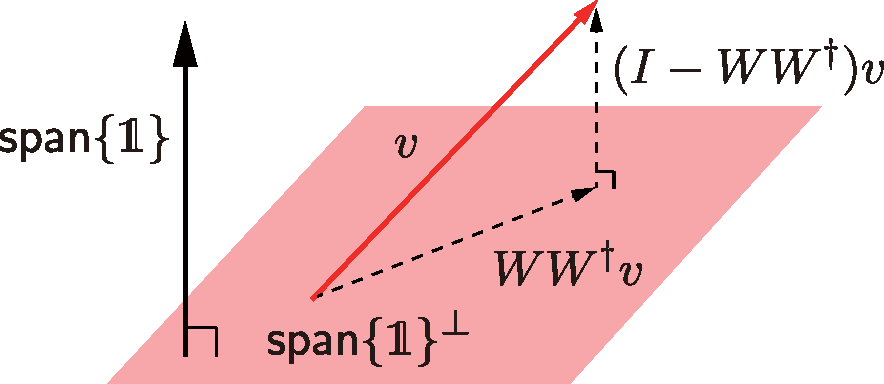
\includegraphics[width = .50\linewidth]{figs/orthogonal}
\medskip
\caption{\textbf{Conceptual diagram of orthogonal projection}}
\label{fig:orthogonal}
\medskip
\end{figure}

We apply the above-mentioned change of basis to the electrical subsystem $G$ of
Equation \ref{eq:Gss}. First, if we substitute Equation \ref{eq:batrinv} into a
differential equation related to $\delta^{\rm lin}$, the following is obtained:

\[
  W
  \dot{\delta}^{\rm lin}_{\rm e} +
  \mathds{1}
  \dot{\overline{\delta}}^{\rm lin}_{\rm e}=u_G
\]

By multiplying the left-hand side of this differential equation by $W^{\dagger}$
or $\tfrac{1}{N} \mathds{1}^{\sf T}$, we obtain:

\[
  \dot{\delta}^{\rm lin}_{\rm e} = W^{\dagger} u_G,\qquad
  \dot{\overline{\delta}}^{\rm lin}_{\rm e} = \frac{1}{N} \mathds{1}^{\sf T} u_G
\]

Next, noting that the relationship in Equation \ref{eq:LBker} holds for matrices
$L$ and $B$, the differential equation and output equation with respect to
$E^{\rm lin}$ can be rewritten as:


\[
  \taud \dot{E}^{\rm lin} = A E^{\rm lin} + 
  B W {\delta}^{\rm lin}_{\rm e}
  , \qquad
  y_G = C E^{\rm lin} + 
  L W {\delta}^{\rm lin}_{\rm e}
\]

Therefore, the transformed electric subsystem is given by:

\begin{equation}\label{eq:Gsstr}
  G: \simode{
  \dot{\overline{\delta}}^{\rm lin}_{\rm e} & = \tfrac{1}{N} \mathds{1}^{\sf T} u_G \\
  \dot{\delta}^{\rm lin}_{\rm e} & = W^{\dagger}u_G \\
  \taud \dot{E}^{\rm lin} &= A E^{\rm lin} + B W {\delta}^{\rm lin}_{\rm e} \\
  y_G &= C E^{\rm lin} + L W {\delta}^{\rm lin}_{\rm e}
  }
\end{equation}

One notable point about this system representation is that the common component
of $\delta^{\rm lin}$, represented by ${\overline{\delta}}^{\rm lin}_{\rm e}$,
is affected by the input $u_G$ but has no effect on the output $y_G$. In other
words, ${\overline{\delta}}^{\rm lin}_{\rm e}$ is an unobservable state
variable.

By removing the differential equation of ${\overline{\delta}}^{\rm lin}_{\rm e}$
from Equation \ref{eq:Gsstr}, $(N-1)$-dimensional controllable and observable
subsystem is obtained as:

\begin{equation}\label{eq:Gsstrmin}
  G_{\rm e}: \simode{
  \dot{\delta}^{\rm lin}_{\rm e} & = W^{\dagger} u_G \\
  \taud \dot{E}^{\rm lin} &= A E^{\rm lin} + B W {\delta}^{\rm lin}_{\rm e} \\
  y_G &= C E^{\rm lin} + L W {\delta}^{\rm lin}_{\rm e}
  }
\end{equation}

Here, please note that from observability of $G_{\rm e}$, the following holds.

\begin{equation}\label{eq:Geobs}
  y_G(t)  =0,\quad \forall t\geq 0 
  \qquad \Longrightarrow \qquad
  \mat{
  {\delta}^{\rm lin}_{\rm e}(t)   \\
  E^{\rm lin}(t)  
  }
  =0
  ,\quad 
  \forall t\geq 0 
\end{equation}

The fact mentioned above is important for the analysis of the steady-state
stability of the approximate linear model in equation \ref{eq:lindynu0}. As a
reference, the block diagram of the approximate linear model transformed by the
change of basis is shown in Figure \ref{fig:GandGe}.

It should be noted that it is a necessary and sufficient condition for $G_{\rm
e}$ to be controllable and observable that the pair $(\taud^{-1}A,\taud^{-1}B)$
is controllable and the pair $(C,\taud^{-1}A)$ is observable. In the following,
we assume controllability and observability. Note that an exact proof is not
always easy, but assuming that the rank of $B$ and $C$ is $(N-1)$ or higher in
most situations, there are no practical obstacles to analysis.

\begin{figure}[t]
  \centering
  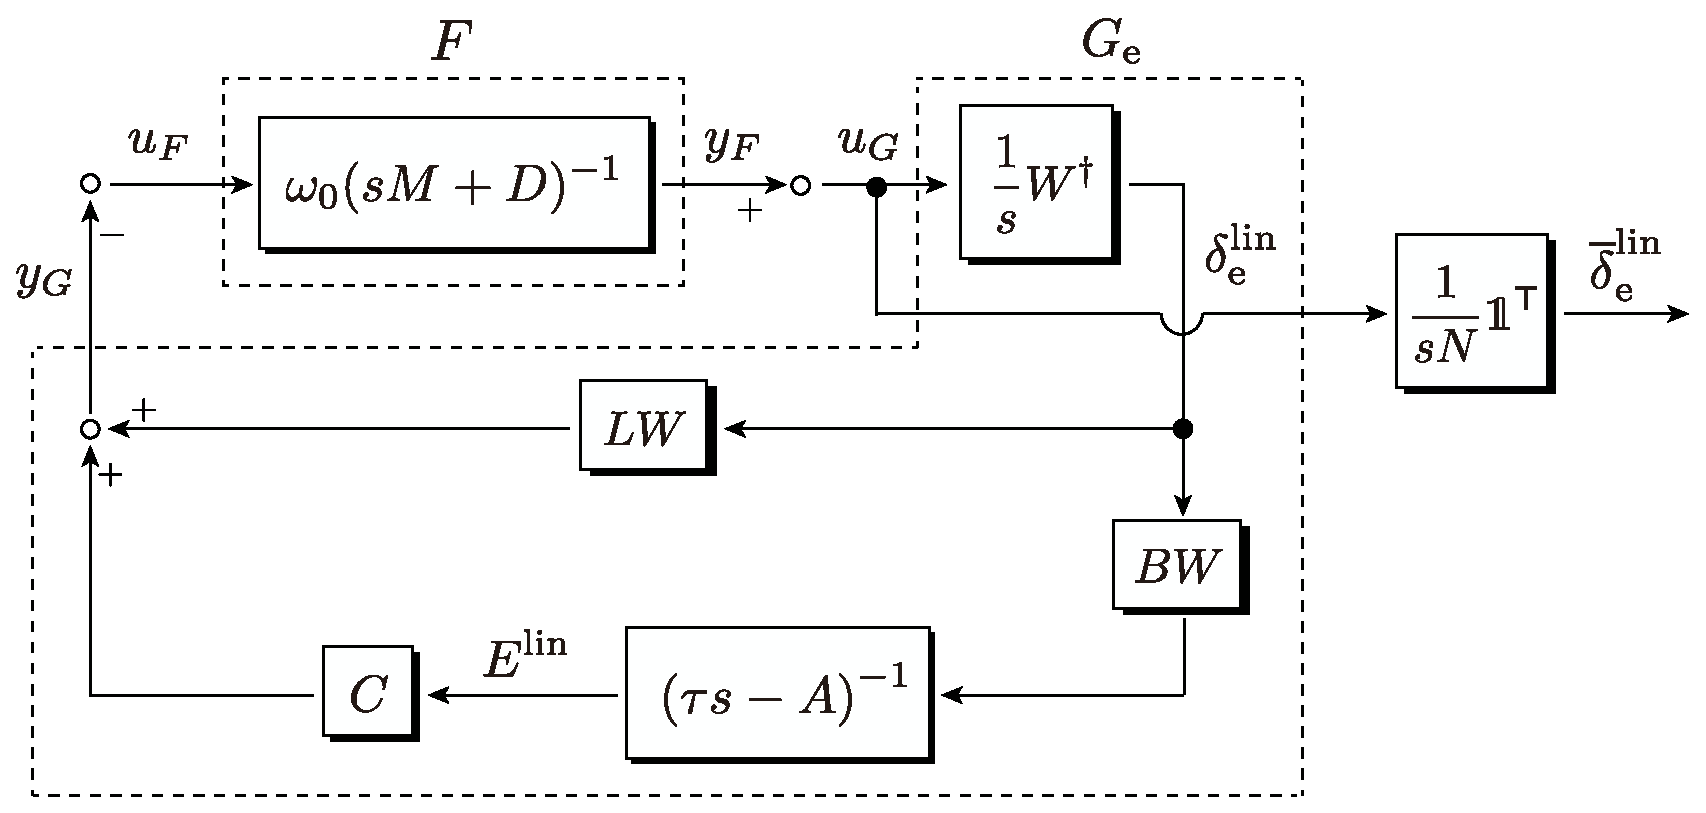
\includegraphics[width = .90\linewidth]{figs/FandGe2}
  \medskip
  \caption{\textbf{Basis-transformed approximate linear model}}
  \label{fig:GandGe}
  \medskip
\end{figure}


\smallskip
\subsubsection{Small signal stability analysis based on passivity}

In the following, assuming the passive power transfer condition defined in
Definition \ref{def:passtrans}, we show the passivity of $G_{\rm e}$ in Equation
\ref{eq:Gsstrmin} using the same procedure as that of the electrical subsystem
$G$ in Equation \ref{eq:Gss}. To this end, we express $G_{\rm e}$ in the form
of:

\begin{equation}\label{eq:Gecomdef}
  G_{\rm e}: \simode{
    \dot{x}_{G_{\rm e}} & = A_{G_{\rm e}} x_{G_{\rm e}} + B_{G_{\rm e}} u_G \\
    y_G &= C_{G_{\rm e}} x_{G_{\rm e}}
  }
\end{equation}

where $x_{G_{\rm e}}$ is a vector composed of ${\delta}^{\rm lin}_{\rm e}$ and
$E^{\rm lin}$, and:

\[
  A_{G_{\rm e}} := 
  \mat{
  0 & 0 \\
  \Omega^2 \hat{B} W  &  \Omega^2 \hat{A} 
  },\quad
  B_{G_{\rm e}} := 
  \mat{
  W^{\dagger} \\
  0
  },\quad
  C_{G_{\rm e}} := 
  \mat{
  LW & -\hat{B}^{\sf T}
}
\]

Additionally, we define the positive semidefinite matrix $P_{G_{\rm e}}$ as:

\begin{equation}\label{eq:defPGe}
  P_{G_{\rm e}} := 
  \mat{
  W & 0 \\
  0 & I
  }^{\sf T}
  \underbrace{
  \mat{
  L  &  - \hat{B}^{\sf T} \\
  - \hat{B} & -\hat{A}
  }
  }_{P_G}
  \mat{
  W & 0 \\
  0 & I
  }
\end{equation}

Note that if $P_G$ in Equation \ref{eq:defPG} is positive semi-definite, then
$P_{G_{\rm e}}$ is also positive semi-definite. In this case, by noting that
$\hat{B}WW^{\dagger}=\hat{B}$ and $LWW^{\dagger}=L$ from the relationship in
Equation \ref{eq:psudinv}, we can see that the following equation holds:

\begin{equation}\label{eq:Gelmi}
  A^{\sf T}_{G_{\rm e}} P_{G_{\rm e}} + P_{G_{\rm e}} A_{G_{\rm e}} \preceq 
  0
  ,\qquad
  P_{G_{\rm e}} B_{G_{\rm e}} = C_{G_{\rm e}}^{\sf T}
\end{equation}

Note that the left matrix inequality is shown from the same equation as
\ref{eq:lyapinG}:

\[
  \frac{
  A^{\sf T}_{G_{\rm e}} P_{G_{\rm e}} + P_{G_{\rm e}} A_{G_{\rm e}}
  }{2}
  =
  \mat{
  \Omega \hat{B}W &0\\
  0 & \Omega^{-1}
  }^{\sf T}
  \underbrace{
  \mat{
  -I & -\hat{A}_{\Omega} \\
  -\hat{A}_{\Omega} & - \hat{A}_{\Omega}^2
  }
  }_{Y}
  \mat{
  \Omega \hat{B}W  &0\\
  0 & \Omega^{-1}
  }
\]

Therefore, the time derivative along the solution trajectory of $G_{\rm e}$ of
the storage function:

\[
  W_{G_{\rm e}}(x_{G_{\rm e}}):= \frac{1}{2}x_{G_{\rm e}}^{\sf T}P_{G_{\rm e}}x_{G_{\rm e}}
\]
can be evaluated as:

\begin{equation}\label{eq:Glyapeq2}
  \frac{d}{dt} W_{G_{\rm e}} \bigl( x_{G_{\rm e}} (t) \bigr)
  \leq 
  y_G^{\sf T}(t) u_G(t)
\end{equation}

Thus, $G_{\rm e}$ in Equation \ref{eq:Gsstrmin} is passive. Note that this
inequality is equivalent to the inequality in Equation \ref{eq:Glyapeq}, and the
values of the two storage functions satisfy:

\[
  W_{G} \bigl( x_{G} (t) \bigr) =
  W_{G_{\rm e}} \bigl( x_{G_{\rm e}} (t) \bigr),\qquad
  \forall t\geq 0
\]

By considering the observability of $G_{\rm e}$ shown by Equation
\ref{eq:Geobs}, the following is true for the arbitrary initial value of the
solution trajectory of the linear approximation model of Equation
\ref{eq:lindynu0}:

\begin{equation}\label{eq:allzero}
  \lim_{t\rightarrow \infty} \Delta \omega^{\rm lin}(t)  =0,\qquad
  \lim_{t\rightarrow \infty} \mat{
  {\delta}^{\rm lin}_{\rm e}(t)   \\
  E^{\rm lin}(t)  
  }
  =0
\end{equation}

Therefore, from the relationship of the change of basis of Equation
\ref{eq:batrinv}, we can see that Equation \ref{eq:linmconv} holds for the
arbitrary initial value. In other words, the linear approximation model of
Equation \ref{eq:lindynu0} is statically stable. Also:

\[
  c_0 = \lim_{t\rightarrow \infty}\overline{\delta}^{\rm lin}_{\rm e}(t)
\]
and state variables $\overline{\delta}^{\rm lin}_{\rm e}$ follow the
differential equation of Equation \ref{eq:Gsstr}.

We summarize the previous discussion in the following theorem.

\begin{theorem}[Small signal stability of the linear approximation model based
on passivity]\label{thm:stasufcon}
For any steady-state value $(\delta^{\star},E^{\star})$ that satisfies the
passive power transfer condition defined in Definition \ref{def:passtrans}, the
electrical subsystem $G$ given in equation \ref{eq:Gss} is passive.
Additionally, for any positive constants $(M_i,D_i,\taudi ){i \in
\mathcal{I}{\rm G}}$, the approximate linear model given in equation
\ref{eq:lindynu0} is steady-state stable.
\end{theorem}

As discussed in Theorem \ref{thm:stasufcon}, under the passive power
transmission conditions, the linear approximation model is statically stable for
combinations of all physical constants $(M_i,D_i,\taudi )_{i \in
\mathcal{I}_{\rm G}}$.  Analysis based on passivity allows stability independent
of model parameters.

\subsection{Necessary conditions for the approxiamte linear model to be
passive\advanced}\label{sec:nesconana}

\smallskip
\subsubsection{Passivity and positive realness}

It is known that the passivity of a linear system is mathematically equivalent
to the property called positive realness of its transfer function. In this
section, we consider the necessity of the passive power transmission condition
defined in Definition \ref{def:passtrans} from the viewpoint of the passivity of
the electrical subsystem based on this equivalence.

\begin{COLUMN}
\noindent \textbf{Transfer function}:
For a linear system:

\begin{equation*}
  \simode{
    \dot{x}(t) & = Ax(t)+Bu(t) \\
    y(t)&= Cx(t) + Du(t)
  }
\end{equation*}
its \textbf{transfer function} is defined as:

\[
  Q(s):=C(sI-A)^{-1}B +D
\]

When the Laplace transform of the input $u(t)$ is $U(s)$ and the Laplace
transform of the output $y(t)$ is $Y(s)$, the transfer function relates to the
system as $Y(s)=Q(s)U(s)$. The input-output behavior of a linear system is
characterized by its transfer function.
\end{COLUMN}

The transfer function from the input $u_G$ to the output $y_G$ of the electrical
subsystem $G$ in Equation \ref{eq:Gss} is given by:

\begin{equation}\label{eq:trGs}
  G(s) :=  - \frac{1}{s} 
  \underbrace{
  \left\{ -C \bigl( \taud s -A \bigr)^{-1} B - L \right\}
  }_{H(s)}
\end{equation}

Note that since unobservable state variables are not relevant to the
input-output characteristics, the transfer function of $G_e$ in Equation
\ref{eq:Gsstrmin} is also equal to $G(s)$. Hereafter, we consider the case where
the transfer function $H(s)$ in Equation \ref{eq:trGs} is stable. The stability
of the transfer function is defined as follows.

\begin{definition}[Stability of a transfer function]\label{def:trsta}
When the real part of all poles of the transfer function $Q(s)$ is negative,
$Q(s)$ is called \textbf{stable}.
\end{definition}

The poles of a transfer function are the zeros of the denominator polynomial. It
is known that $H(s)$ in equation \ref{eq:trGs} being stable is equivalent to all
the real parts of the eigenvalues of the matrix $\taud^{-1}A$ being negative.

Furthermore, the \textbf{Positive realness} of a transfer function is defined as
follows.

\begin{definition}[Positive realness of a transfer function]\label{def:trpf}
For a square transfer function $Q(s)$, the following is defined:

\begin{equation}\label{eq:defOm0}
  \Omega_0 := \left\{
  \omega_0 \in \mathbb{R}: 
  \mbox{ The pure imaginary number $\bm{j} \omega_0$ is a pole of $Q(s)$}
  \right\}
\end{equation}

$Q(s)$ is called \textbf{positive real} if the following three conditions are
satisfied.

\begin{itemize}
  \item The real part of all poles of $Q(s)$ is nonpositive.
  \item For all $\omega \in [0,\infty)\setminus \Omega_0$, $Q(\bm{j} \omega) + Q^{\sf T}(-\bm{j} \omega)$ is positive semi-definite.
  \item When there are poles of a pure imaginary number, their multiplicity is 1, and the following is true for the remaining number: 
  \begin{equation*}
    \lim_{s \rightarrow \bm{j} \omega_0} (s-\bm{j} \omega_0) Q(s) = \lim_{s\rightarrow \bm{j} \omega_0} \{ (s-\bm{j} \omega_0) Q(s)\}^{\sf *}\succeq 0
    ,\qquad
    \forall \omega_0 \in \Omega_0
  \end{equation*}
\end{itemize}
\end{definition}

In Definition \ref{def:trpf}, the two most important conditions are the first
and second ones. The first condition expresses the stability of the transfer
function. However, it also includes the case where the real part of the pole is
0. The second condition concerns the positive definiteness of the complex
symmetric part of the transfer function evaluated on the imaginary axis. In
particular, if $Q(s)$ is a scalar, that is, both the input and output are
scalars, the second condition expresses that the real part of $Q(\bm{j}\omega)$
is non-negative for all $\omega \in [0,\infty)\setminus \Omega_0$. However, it
should be noted that for matrix-valued $Q(s)$, in general,

\begin{equation*}
  Q(\bm{j} \omega) + Q^{\sf T}(-\bm{j} \omega) \neq 2 \real\left[ Q(\bm{j} \omega) \right]
\end{equation*}

Also, for $Q(s)$ with real coefficients, $Q^{\sf T}( -\bm{j} \omega)$ is equal
to ${Q(\bm{j} \omega)}^*$. The third condition is exceptional in the case when
$Q(s)$ has pure imaginary poles. However, it is necessary to analyze transfer
functions with poles at the origin, such as $G(s)$ in Equation \ref{eq:trGs}.

\begin{COLUMN}
\noindent \textbf{Complex Symmetric and Skew Hermitian Parts of a Square Matrix}:
Any square matrix $M$ can be decomposed as:

\[
M=\frac{M+M^*}{2}+\frac{M-M^*}{2}
\]
where $\tfrac{M+M^*}{2}$ is called the \textbf{complex symmetric part} (Hermitian
part) \index{Hermitian part} of $M$, and $\tfrac{M-M^*}{2}$ is called the
\textbf{complex skew-symmetric part} (skew Hermitian part) \index{skew Hermitian
part} of $M$.
\end{COLUMN}

In system control engineering, it is known that passivity in Definition
\ref{def:passivelin} and positive realness in Definition \ref{def:trpf} are
equivalent. If we apply Lemma \ref{lem:prlem} at the end of this chapter to the
discussion in this section, the necessary and sufficient condition for $G(s)$ in
Equation \ref{eq:trGs} to be positive real is the existence of a positive
definite matrix $P_{G_{\rm e}}$ that satisfies Equation \ref{eq:allzero} for the
controllable and observable state space realization $G_{\rm e}$ in Equation
\ref{eq:Gecomdef}. This is equivalent to the passivity of $G_{\rm e}$ defined by
the inequality in Equation \ref{eq:Glyapeq2}. Furthermore, the positive
realness of $P_{G_{\rm e}}$ in Equation \ref{eq:defPGe} is shown by the fact
that both the Schur complements with respect to $-\hat{A}$ and $-\hat{A}$ of the
matrix $W^{\sf T} \left(L+\hat{B}^{\sf T} \hat{A}^{-1} \hat{B} \right) W$ are
positive definite, where $W^{\sf T} L_0 W$ satisfies Equation \ref{eq:nescon}
and the column vectors of $W$ in Equation \ref{eq:batrinv} are orthogonal to
$\mathds{1}$.

\smallskip
\subsubsection{Necessary condition for the transfer function of the electrical
subsystem to be positive-real}

As a mathematical preparation for deriving necessary conditions, we introduce
the concept of \textbf{negative imaginaryness}\index{negative imaginaryness} of
transfer functions, which is similar to positive-realness
\cite{petersen2010feedback,xiong2010negative}.

\begin{definition}[Negative imaginariness of a transfer function]
  \label{def:trni}
  For a square transfer function $Q(s)$ without a pole at the origin, we define $\Omega_0$ of Equation \ref{eq:defOm0}.
  When the following three conditions are satisfied, $Q(s)$ is called \textbf{negative imaginary}.
  \begin{itemize}
    \item The real part of all poles of $Q(s)$ is nonpositive.
    \item For all $\omega \in (0,\infty)\setminus \Omega_0$, $\bm{j}\left\{Q(\bm{j} \omega) - Q^{\sf T}(-\bm{j} \omega) \right\}$ is positive semi-definite.
    \item When there is a pole of a pure imaginary number, their multiplicity is 1, and the following holds for the remaining numbers:
    \begin{equation*}
      \lim_{s \rightarrow \bm{j} \omega_0} (s-\bm{j} \omega_0) \bm{j} Q(s) = 
      \lim_{s\rightarrow \bm{j} \omega_0} \{ (s-\bm{j} \omega_0) \bm{j} Q(s)\}^{\sf *}\succeq 0
      ,\quad
      \forall \omega_0 \in \Omega_0
    \end{equation*}
  \end{itemize}
\end{definition}

While Definition \ref{def:trpf} defines positive-realness based on the
positive-definiteness of the complex symmetric part of a transfer function,
Definition \ref{def:trni} defines negative-imaginaryness based on the
positive-semidefiniteness of the complex anti-symmetric part of the transfer
function multiplied by the imaginary unit. Note that since the eigenvalues of a
complex anti-symmetric matrix are purely imaginary, their product with the
imaginary unit is real. In particular, when $Q(s)$ is a scalar transfer
function, the second condition implies that the imaginary part of
$Q(\bm{j}\omega)$ is non-positive for all $\omega \in (0,\infty)\setminus
\Omega_0$. Furthermore, in the following discussion, we focus only on the second
condition to consider the negative-imaginaryness of stable transfer functions.
Similar to positive-realness, negative-imaginaryness can also be characterized
as the solvability of matrix inequalities, as described in Lemma \ref{lem:nilem}
at the end of this chapter.

\begin{figure}[t]
  \centering
  {
  \begin{minipage}{0.49\linewidth}
    \centering
    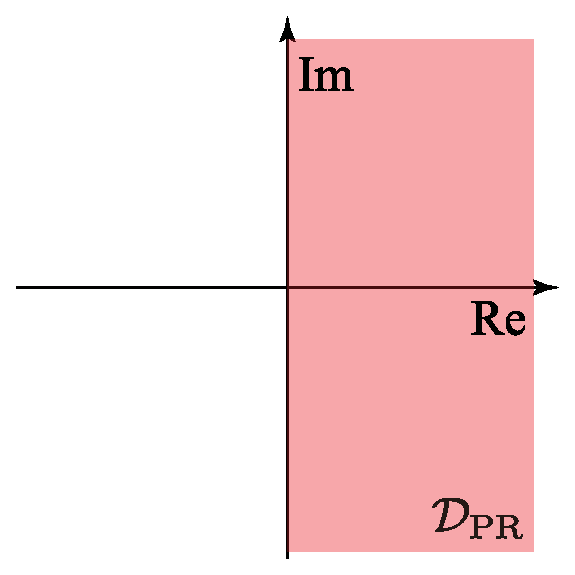
\includegraphics[width = .65\linewidth]{figs/PRdom}
    \subcaption{ $\mathcal{D}_{\rm PR}$ }
    \medskip
  \end{minipage}
  \begin{minipage}{0.49\linewidth}
    \centering
    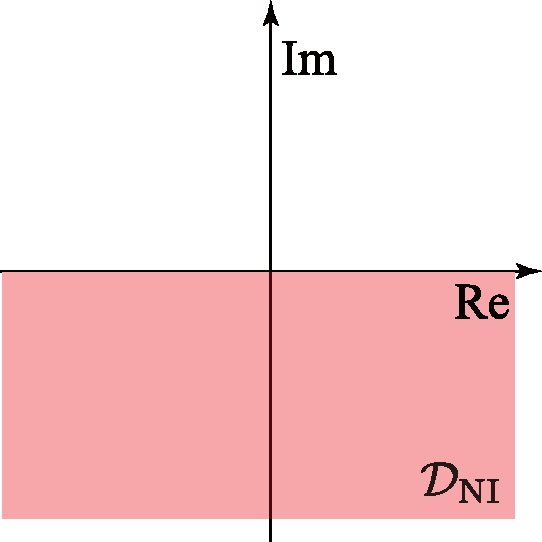
\includegraphics[width = .65\linewidth]{figs/NIdom}
    \subcaption{ $\mathcal{D}_{\rm NI}$ }
    \medskip
  \end{minipage}
  }
  \medskip
  \caption{\textbf{Positive realms and negative imaginary realms}}
  \label{fig:PRandNI}
\medskip
\end{figure}


\begin{COLUMN}
\noindent \textbf{Nyquist plot}:
The plot of the frequency response function $Q(\bm{j}\omega)$ for
$\omega\in\mathbb{R}$ on the complex plane is called the \textbf{Nyquist
plot}\index{Nyquist plot}. It is often used in geometric analysis of stability
for feedback systems. The analysis method is called the \textbf{Nyquist
stability criterion}\index{Nyquist stability criterion}. Note that when $Q(s)$
is a scalar and the coefficients of the numerator and denominator polynomials
are real, the plot of $Q(\bm{j}\omega)$ for negative $\omega$ is symmetrical to
the plot for positive $\omega$ with respect to the real axis.
\end{COLUMN}

The relationship of positive realness and negative imaginariness is explained
with Figure \ref{fig:PRandNI}. If the transfer function $Q(s)$ is scalar,
$Q(s)$ being positive real can be understood as the trajectory related to
non-negative $\omega$ of the frequency response function $Q(\bm{j} \omega)$ is
included in the range $\mathcal{D}_{\rm PR}$ shown in \ref{fig:PRandNI}(a).

\[
  \mathcal{D}_{\rm PR} = \bm{j} \mathcal{D}_{\rm NI}
\]

and $-\tfrac{1}{\bm{j}}=\bm{j}$ for $G(s)$ and $H(s)$ of Equation \ref{eq:trGs},
the following is derived:

\[
  G(\bm{j} \omega) \in \mathcal{D}_{\rm PR}, 
  \quad \forall \omega >0
  \qquad
  \Longleftrightarrow
  \qquad
  H(\bm{j} \omega) \in \mathcal{D}_{\rm NI} ,
  \quad \forall \omega >0
\]

Therefore, a negative imaginariness analysis of $H(s)$ is equivalent to a
positive realness analysis of $G(s)$. To be accurate, $G(\bm{j} \omega)$ and
$H(\bm{j} \omega)$ are complex matrices; thus, $\mathcal{D}_{\rm PR}$ and
$\mathcal{D}_{\rm NI}$ should be redefined with a set of positive semi-definite
matrices.

Therefore, a negative imaginariness analysis of $H(s)$ is equivalent to a
positive realness analysis of $G(s)$. Based on this fact, the passive power
transmission conditions (ii) and (iii) are necessary conditions for $G(s)$ to be
positive real.

\begin{theorem}{Positive realness of electrical subsystem transfer function}
\label{thm:EdynNI}
For any $(\delta^{\star},E^{\star})$ where the transfer function $H(s)$ given by
Equation \ref{eq:trGs} is stable, a necessary and sufficient condition for
$H(s)$ to be negative imaginary is that the passive power transmission condition
(ii) in Definition \ref{def:passtrans} holds. Furthermore, a necessary and
sufficient condition for the transfer function $G(s)$ given by Equation
\ref{eq:trGs} to be positive real is that both passive power transmission
conditions (ii) and (iii) in Definition \ref{def:passtrans} hold.
\end{theorem}

\begin{proof}
First, we show that if $H(s)$ is negative imaginary for any
$(\delta^{\star},E^{\star})$ where $H(s)$ is stable, then the passive power
transmission condition (ii), which is expressed in equation \ref{eq:Gredcon},
holds true. Now, since:

\[
  \lim_{\omega \rightarrow \infty} \bm{j}
  \left\{
  H(\bm{j}\omega)-H^{\sf T}(-\bm{j}\omega)
  \right\}
  =\bm{j}
  \left(
  -L+L^{\sf T}
  \right) \succeq 0
\]

$L$ must be symmetric for $H(s)$ to be negative imaginary. Therefore, we obtain
$k_{ij}(\delta_{ij}^{\star}) = k_{ji}(\delta_{ji}^{\star})$.

Therefore, $L$ must be symmetric for $H(s)$ to be negative vacuity.
Thus, we have $K_{IJ}(\delta_{IJ}^{\star}) = K_{JI}(\delta_{JI}^{\star})$.

In other words:
\[
  G^{\rm red}_{ij} \sfsin \delta_{ij}^{\star} = 0 ,\qquad
  \forall (i, j) \in \mathcal{I}_{\rm G} \times \mathcal{I}_{\rm G}
\]

This implies $\delta_{i}^{\star}\neq \delta_{j}^{\star}$ for $(i,j)$ where
$G^{\rm red}_{ij}=0$. Also, even in the case where $\delta_{i}^{\star}=
\delta_{j}^{\star}$, there exists a sufficiently small $\gamma>0$ such that
$\taud^{-1}A$ is stable for $\delta^{\star}+\gamma e_i$ due to the continuity of
the eigenvalue parameter variation for matrices with parameters. Here, $e_i$
represents a vector with only the $i$-th element being 1 and the others being 0.
Therefore, we obtain:

\begin{equation}\label{eq:Gij0t}
  G^{\rm red}_{ij}=0, \qquad
  \forall i\neq j
\end{equation}

Furthermore, if $H(s)$ is negative imaginary, then $L_0$ in equation
\ref{eq:defL0} must also be symmetric, because we have:

\[
  \lim_{\omega \rightarrow 0} \bm{j}
  \left\{
  H(\bm{j}\omega)-H^{\sf T}(-\bm{j}\omega)
  \right\}
  =\bm{j}
  \left(
  -L_0+L_0^{\sf T}
  \right) \succeq 0
\]

When equation \ref{eq:Gij0t} holds, it should be noted that $L_0$ can be
expressed as follows:

\[
  C = \sfdiag \left(
  2E_i^{\star} G^{\rm red}_{ii}
  \right)  - \hat{B}^{\sf T}
  \]
  Note that $L_0$ is given by:
  \[
  L_0 = \underbrace{ L + \hat{B}^{\sf T} \hat{A}^{-1} \hat{B} }_{L_1}
  -
  \underbrace{ \sfdiag (
  2 E_i^{\star} G^{\rm red}_{ii}
  ) \hat{A}^{-1} \hat{B}
  }_{L_2}
\]
where $\hat{A}$ is a symmetric matrix defined in equation \ref{eq:sysmats}.
Therefore, $L_1$ is symmetric. On the other hand, for $L_2$ to be symmetric for
any $E^{\star}$, it must be the case that $G^{\rm red}_{ii} \neq 0$ for all $i$.
From this, it follows that if $H(s)$ is negative imaginary for any
$(\delta^{\star},E^{\star})$ such that $H(s)$ is stable, then equation
\ref{eq:Gredcon} holds.

Next, we will show that if Equation \ref{eq:Gredcon} holds, then $H(s)$ is
negative imaginary for any $(\delta^{\star},E^{\star})$ that makes $H(s)$
stable. For this purpose, it is enough to show that there exists a positive
definite matrix $P$ that satisfies $L$ is symmetric and

\begin{equation}\label{eq:cndQ}
  \tilde{A}^{\sf T}P + P\tilde{A} \preceq 0
  ,\qquad
  P\tilde{A}^{-1}\tilde{B}=C^{\sf T}
\end{equation}

\begin{equation*}
  \tilde{A}:= \taud^{-1}A
  ,\qquad
  \tilde{B}:= \taud^{-1}B
\end{equation*}

Note that if equation \ref{eq:Gredcon} holds, then

\begin{equation*}
  k_{ij}(\delta_{ij}^{\star}) =
  k_{ji}(\delta_{ji}^{\star})
  ,\qquad
  h_{ij}(\delta_{ij}^{\star}) = 
  - h_{ji}(\delta_{ji}^{\star}),\qquad
  h_{ii}(\delta_{ii}^{\star}) = 0
\end{equation*}
which implies that $L$ is symmetric. Moreover, since $H(s)$ is stable, we have

\begin{equation*}
  \tilde{A} = 
  \sfdiag \left( \frac{ \Xsi -  \Xti }{ \taudi } \right)
  \hat{A}
\end{equation*}
and since $\Xsi > \Xti$, the matrix $\hat{A}$ in Equation \ref{eq:sysmats} is
negative definite. Therefore, we can choose $P=-\hat{A}$ as a positive definite
matrix that satisfies Equation \ref{eq:cndQ}, which implies that $H(s)$ is
negative imaginary.

Next, we show the equivalence of $G(s)$. Since $H(s)$ is stable, the poles of
$G(s)$ on the imaginary axis are only at the origin and have a multiplicity of
1. Therefore, the necessary and sufficient condition for $G(s)$ to be positive
real is:

\begin{equation}\label{eq:Gpr}
  G(\bm{j}\omega) + G^{\sf T}(-\bm{j}\omega) \succeq 0
  ,\qquad \forall \omega \in \mathbb{R}\setminus\{0\}
\end{equation}

Then the following can be established:

\begin{equation}\label{eq:cndG0}
  \lim_{s\rightarrow 0} s G(s) = \lim_{s\rightarrow 0} \{ s G(s)\}^{\sf T}\succeq 0
\end{equation}

When the Equation \ref{eq:Gredcon} holds, then the Equation \ref{eq:Gpr} holds.

\begin{equation}\label{eq:NIineq}
  G(\bm{j}\omega) + G^{\sf T}(-\bm{j}\omega)
  =
  \frac{\bm{j}}{\omega} \left\{
  H(\bm{j}\omega) - H^{\sf T}(-\bm{j}\omega)
  \right\}
  ,\qquad \forall \omega \in \mathbb{R}\setminus\{0\}
\end{equation}

It is shown from $H(s)$ that $H(s)$ is negative imaginary. Moreover: 

\begin{equation*}
  \lim_{s\rightarrow 0} s G(s) =
  L - C\tilde{A}^{-1}\tilde{B} = L - C A^{-1} B
\end{equation*}

Therefore, the positive semi-dfiniteness of equation \ref{eq:cndG0} is
equivalent to the passive transmission condition (iii), i.e., the condition of
Equation \ref{eq:pdsp}. Note that when the passive transmission condition (ii)
holds, $L$ is symmetric and:

\begin{equation*}
  C\tilde{A}^{-1}\tilde{B} = C P^{-1} C^{\sf T}
\end{equation*}
is also symmetric, which also shows the symmetry of the expression
\ref{eq:cndG0}.

On the contrary, if either the passive power transmission condition (ii) or
(iii) is not satisfied, it indicates that $G(s)$ is not positive real. As for
the latter, it is evident from the fact that the condition in Equation
\ref{eq:pdsp} is equivalent to the condition in Equation \ref{eq:cndG0}.
Additionally, when the passive power transmission condition (ii) is not
satisfied, $H(s)$ is not purely imaginary, and there exist some point
$\omega_0\geq 0$ and sufficiently small $\epsilon >0$ such that:

\begin{equation*}
  \lambda_{\rm min}\left[
  \bm{j}
  \left\{
  H(\bm{j}(\omega_0 + \alpha )) - H^{\sf T}(-\bm{j}(\omega_0 + \alpha ))
  \right\}
  \right] < 0
  ,\qquad
  \forall \alpha \in (0,\epsilon] 
\end{equation*}

where $\lambda_{\rm min}$ denotes the minimum eigenvalue. Therefore, for all
non-zero $\omega \in (\omega_0, \omega_0+\epsilon]$, the complex symmetric part
of $G(\bm{j} \omega)$ is not semi-positive definite.
\end{proof}

\begin{figure}[t]
  \centering
  {
  \begin{minipage}{0.49\linewidth}
    \centering
    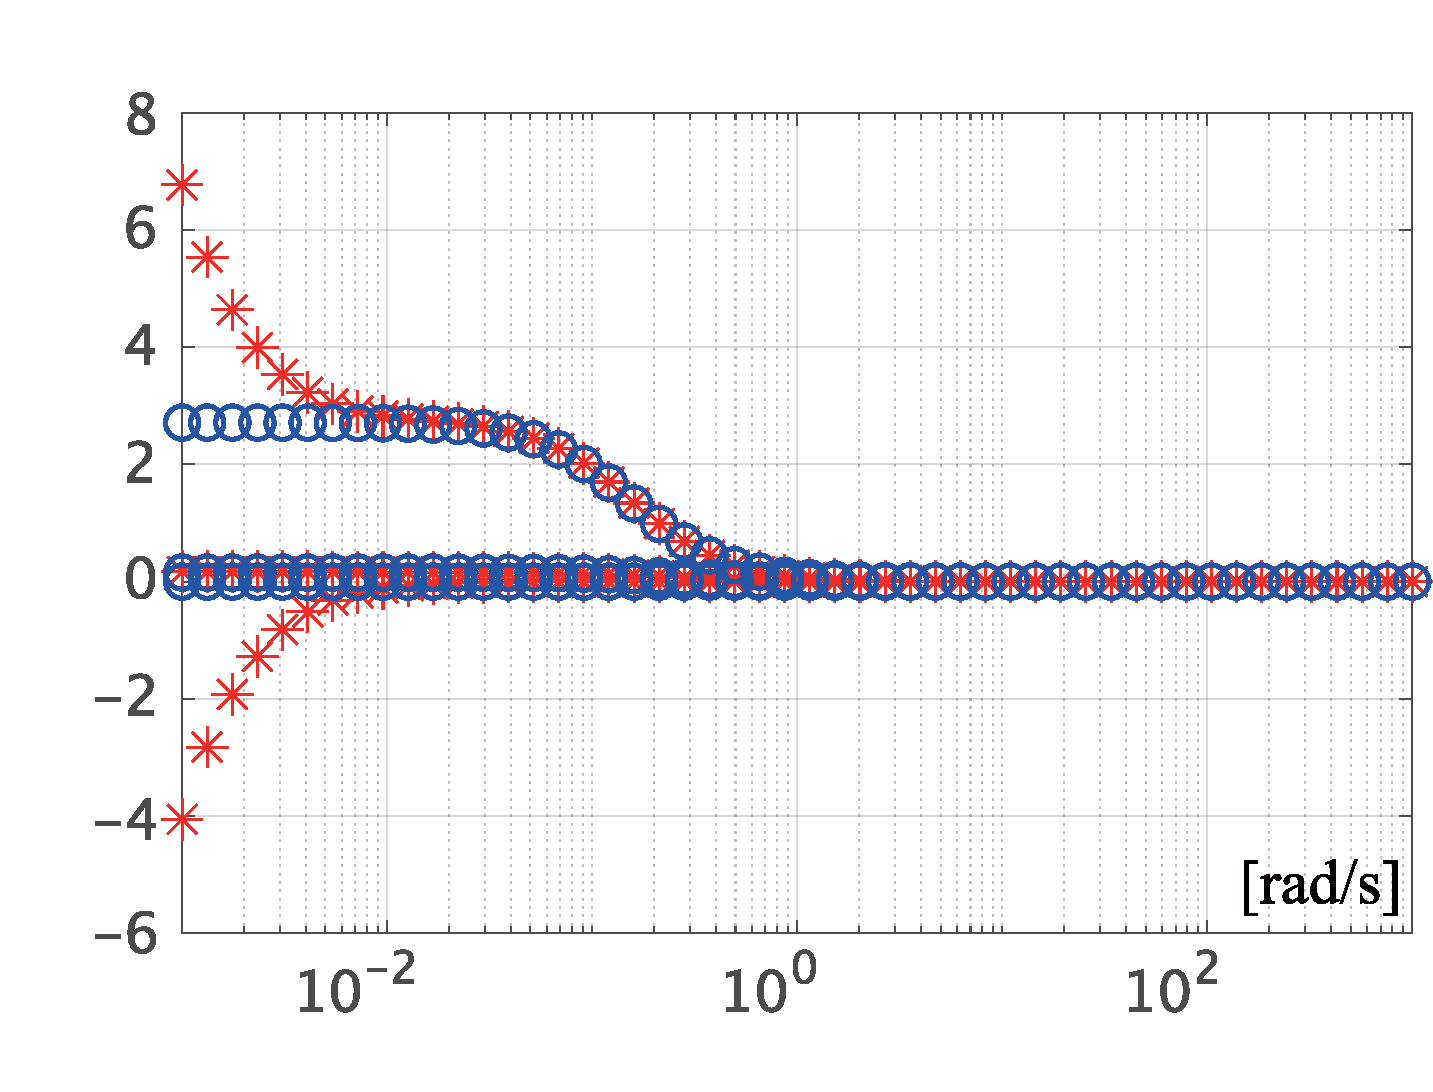
\includegraphics[width = 1.0\linewidth]{figs/eigG}
    \subcaption{ Eigenvalue of $\tfrac{G(\bm{j} \omega) + G^{\sf T}(-\bm{j} \omega)}{2} $}
    \medskip
  \end{minipage}
  \begin{minipage}{0.49\linewidth}
    \centering
    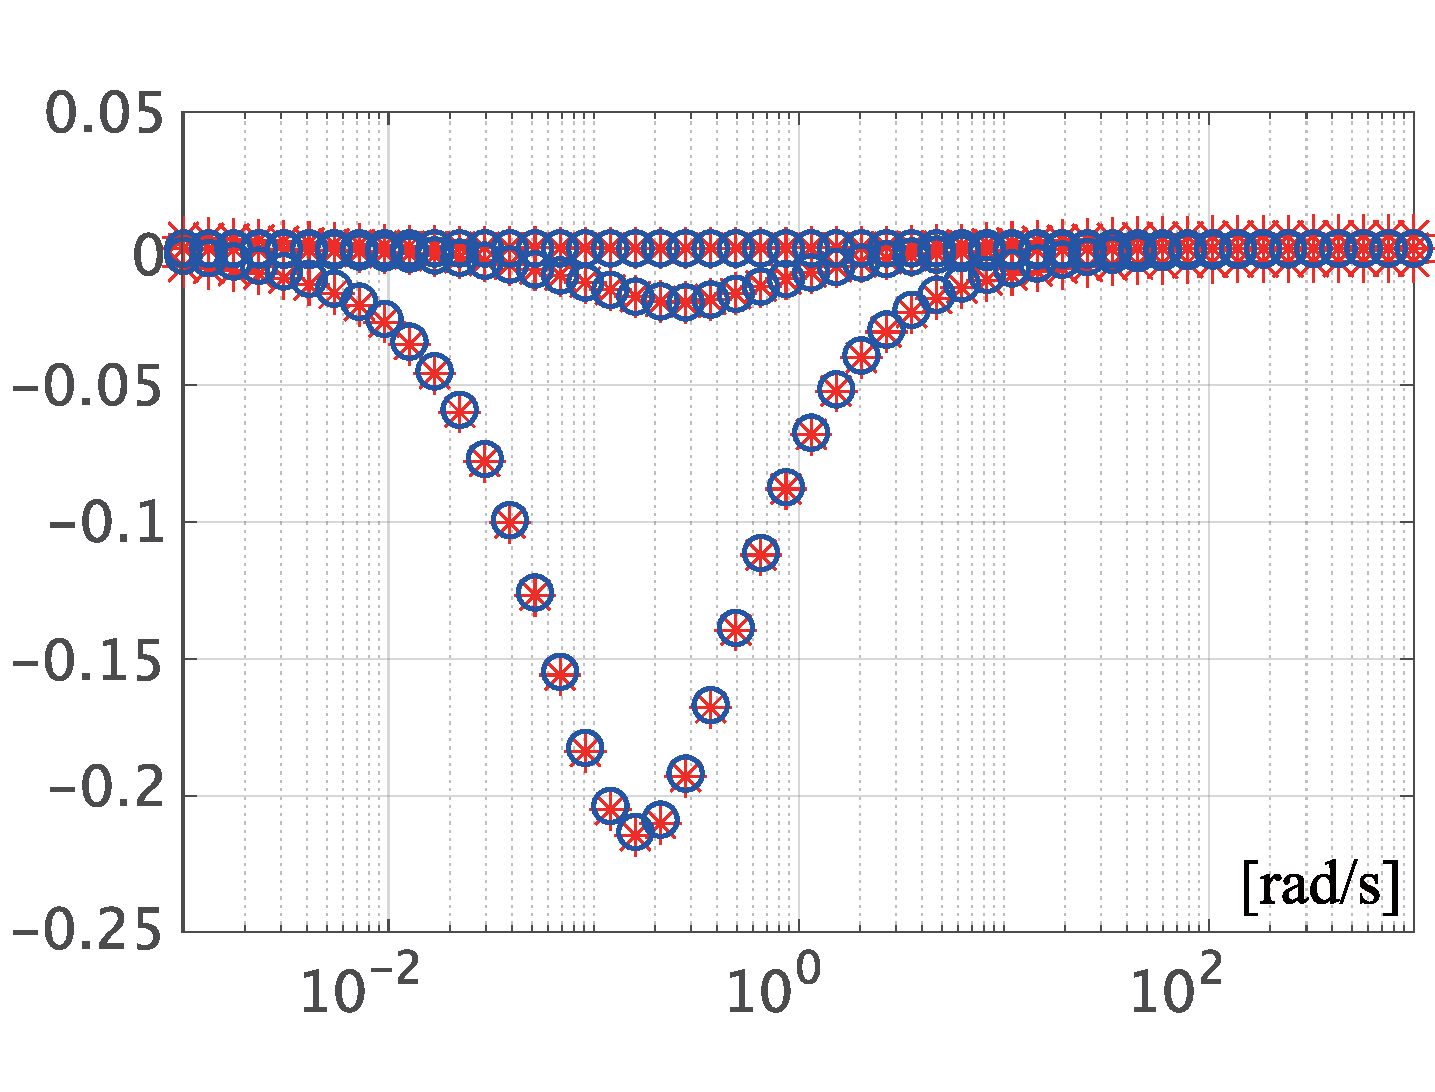
\includegraphics[width = 1.0\linewidth]{figs/eigH}
    \subcaption{ Eigenvalue of $\tfrac{H(\bm{j}\omega) - H^{\sf T}(-\bm{j}\omega)}{2\bm{j}}$}
    \medskip
  \end{minipage}
  }
  \medskip
  \caption{\textbf{Positive realness of $\bm{G(s)}$ and negative imaginariness of$\bm{H(s)}$}
  \\  \centering(Blue: passive transmission condition (ii) is satisfied, Red: not satisfied)}
  \label{fig:eigGH}
\medskip
\end{figure}

Let us confirm the result of Theorem \ref{thm:EdynNI} with the following
example.

\begin{example}{Transmission loss and positive realness of transfer function of
electrical subsystem}

Let's examine the positive realness of $G(s)$ and the negative imaginary
property of $H(s)$ for the power system model composed of three generators that
we dealt with in Example \ref{ex:linsyssim}. We will calculate these properties
in two cases: when the passive power transmission condition (ii) is satisfied
and when it is not, for comparison purposes. Specifically, as in Example
\ref{ex:energylin}, we set two types of $\bm{Y}_0(0)$ and $\bm{Y}_0(1)$ as the
admittance matrix $\bm{Y}$ of the transmission network. The eigenvalues of the
complex symmetric part of $G(\bm{j}\omega)$ and the imaginary parts of the
eigenvalues of the complex skew-symmetric part of $H(\bm{j}\omega)$ are plotted
against the frequency $\omega$ on the horizontal axis in Figure
\ref{fig:eigGH}(a) and Figure \ref{fig:eigGH}(b), respectively. The blue circles
indicate when the passive power transmission condition (ii) is satisfied, and
the red asterisks indicate when it is not. From this figure, we can see that if
the conductance of the transmission lines is non-zero, the complex symmetric
part of $G(\bm{j}\omega)$ is not semi-positive definite in the low-frequency
band.  \end{example}

The meaning of the passive power transmission condition (iii), which appeared as
a condition for $P_G$ in Equation \ref{eq:defPG} to be semi-positive definite,
can also be explained as follows. Consider the state equation of the internal
voltage in the electrical subsystem $G$ given in Equation \ref{eq:Gss}:

\begin{equation*}
  \taud
  \dot{E}^{\rm lin} = 
  A E^{\rm lin} + B \delta^{\rm lin}
\end{equation*}

Let us focus on the limit where the time constant $( \taudi )_{i \in
\mathcal{I}_{\rm G}}$ tends to 0. This corresponds to considering the limit where
"the time it takes for the internal voltage to reach a steady state is much
shorter than the variation of $\delta^{\rm lin}$." In this case, the following
approximation holds:

\begin{equation}\label{eq:spa}
  E^{\rm lin}(t) \simeq  -A^{-1} B\delta^{\rm lin}(t)
  ,\qquad
  \forall t\geq 0
\end{equation}

However, if $A$ is unstable, i.e., if the passive power transmission condition
(i) does not hold, the state $E^{\rm lin}$ diverges. Systems with state
variables that have different time scales are called \textbf{singularly
perturbed systems} \cite{kokotovic1987singular} in the field of control
engineering. A differential equation system with sufficiently small time
constants can be approximated by an algebraic equation system. In fact, the
dynamic characteristics of internal voltage often have smaller time constants
than the mechanical turbine dynamics.

Assuming that equation \ref{eq:spa} holds as an equality, substituting it into
the output equation of equation \ref{eq:Gss} yields a low-dimensional
approximation of the electrical subsystem as follows:

\begin{equation}\label{eq:Gsssp}
  \hat{G}: \simode{
    \dot{\hat{\delta}}^{\rm lin} & = u_G \\
    y_G &= L_0 \hat{\delta}^{\rm lin}
  }
\end{equation}

However, to indicate that this is an approximation, the state variable is
distinguished as $\hat{\delta}^{\rm lin}$.

Using the low-dimensional approximation of this singular perturbation system,
the entire approximate linear model of equation \ref{eq:lindynu0} is
approximated as a system of coupled differential equations with two second-order
oscillators:

\begin{equation}\label{eq:spamodel}
  M \ddot{\hat{\delta}}^{\rm lin}
  + D \dot{\hat{\delta}}^{\rm lin}
  +\omega_0 L_0 \hat{\delta}^{\rm lin}=0
\end{equation}

From this result, it can be understood that the passive power transmission
condition (iii) represents the "semi-positive definiteness of the spring
constant matrix" in the case of small time constants. Furthermore, the
electrical subsystem $G$ of Equation \ref{eq:Gss} can be interpreted as
corresponding to a dynamic spring constant.

\begin{figure}[t]
  \centering
  {
  \begin{minipage}{0.49\linewidth}
    \centering
    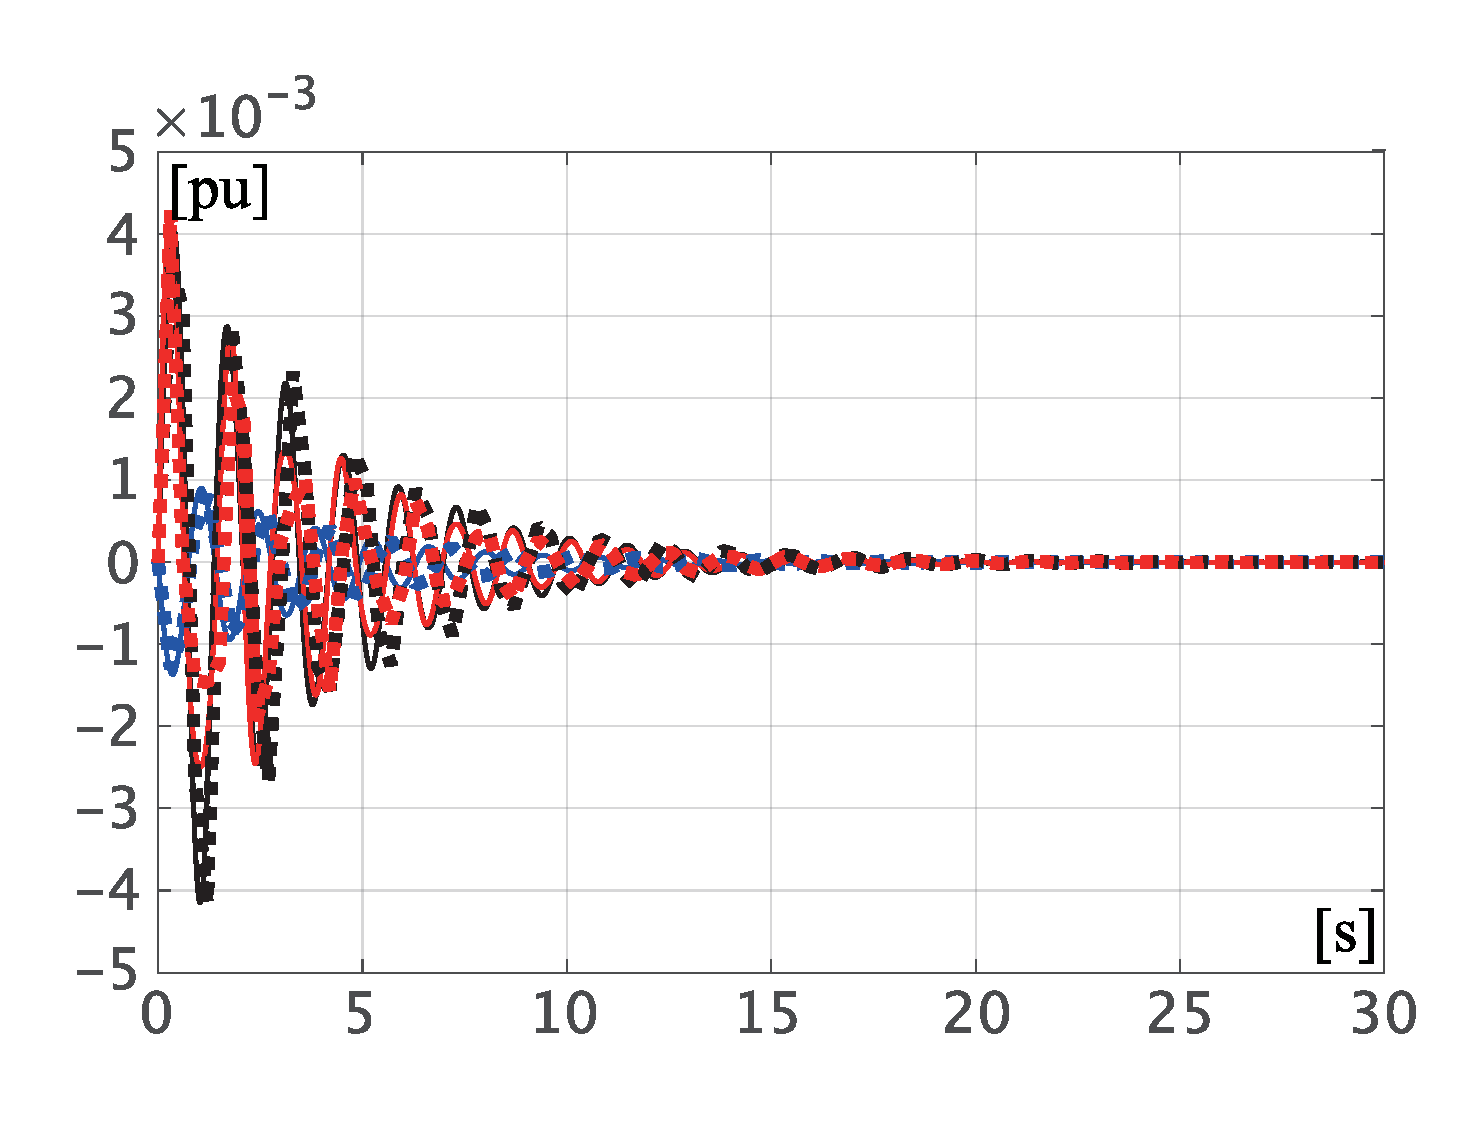
\includegraphics[width = 1.0\linewidth]{figs/Domegaspa}
    \subcaption{ Solid line: $\Delta \omega^{\rm lin}$, Dotted line: $\Delta \hat{\omega}^{\rm lin}$ }
    \medskip
  \end{minipage}
  \begin{minipage}{0.49\linewidth}
    \centering
    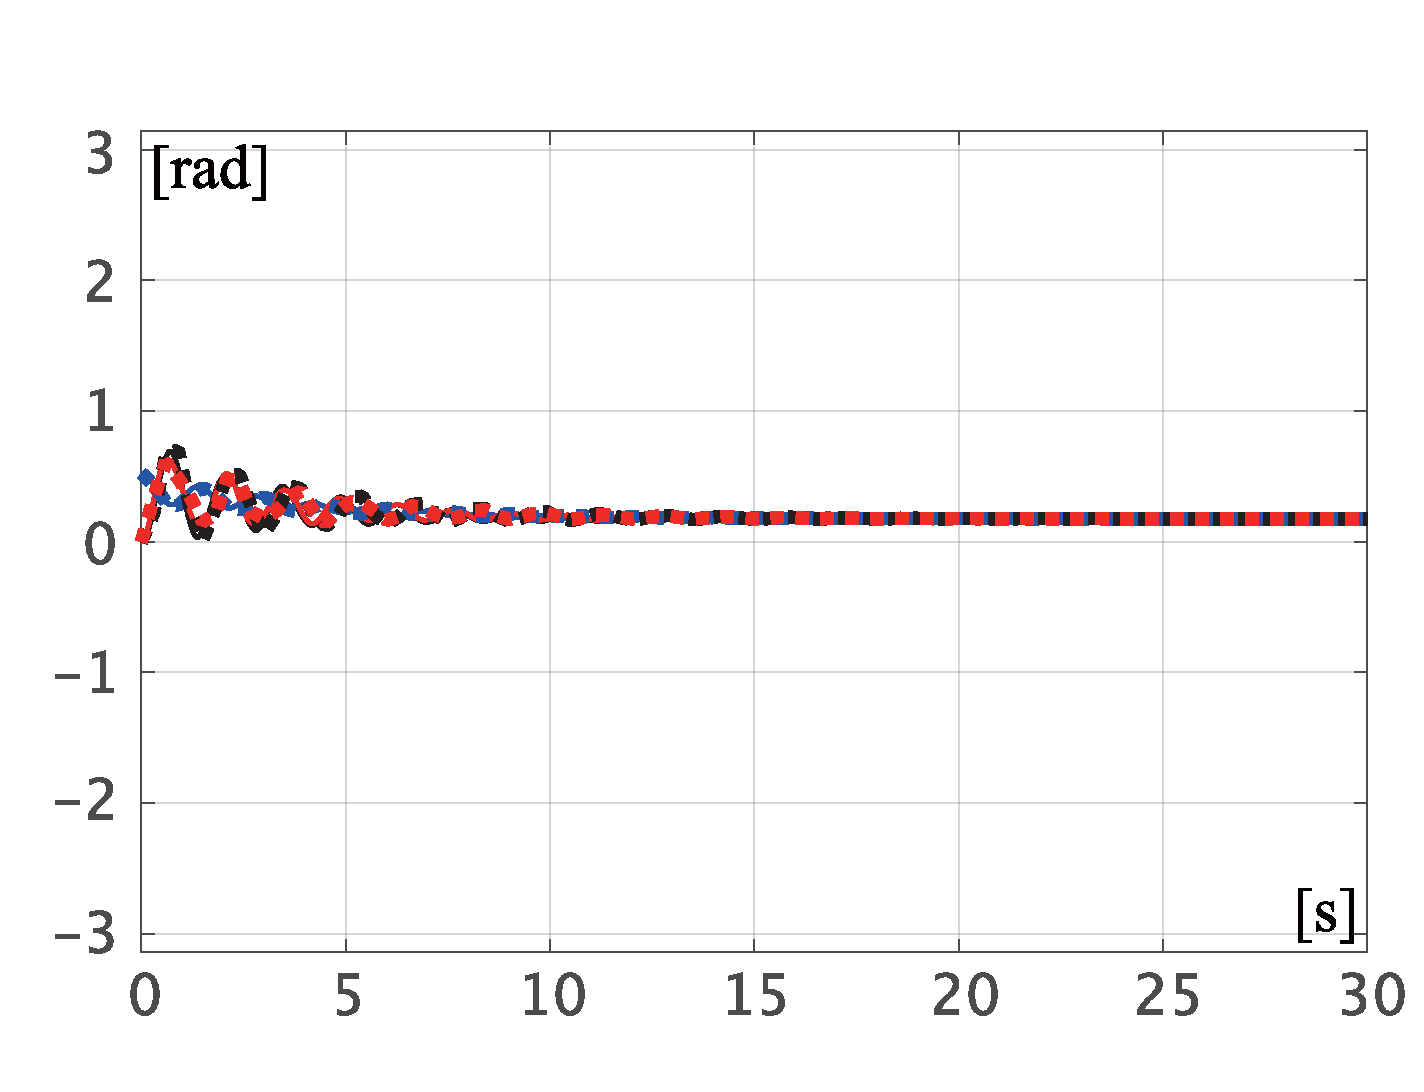
\includegraphics[width = 1.0\linewidth]{figs/deltaspa}
    \subcaption{ Solid line:$\delta^{\rm lin}$, Dotted line:${\hat{\delta}}^{\rm lin}$ }
    \medskip
  \end{minipage}
 \begin{minipage}{0.49\linewidth}
    \centering
    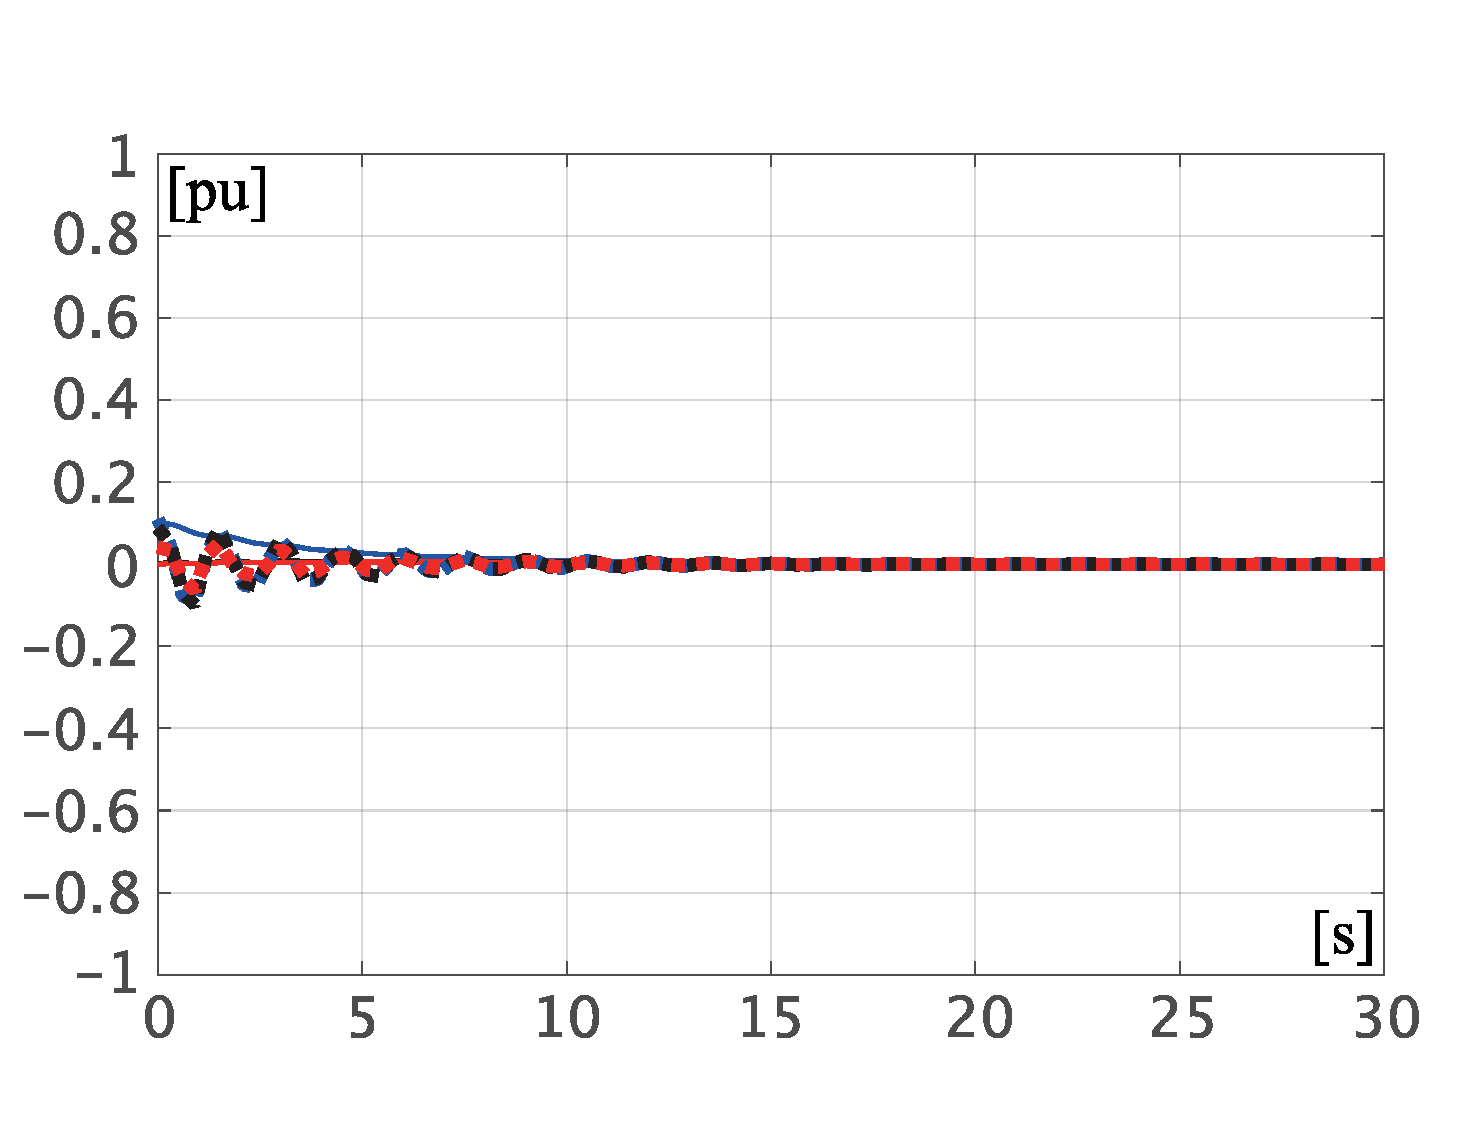
\includegraphics[width = 1.0\linewidth]{figs/Espa}
    \subcaption{ Solid line:$E^{\rm lin}$, Dotted line:$\hat{E}^{\rm lin}$ }
    \medskip
  \end{minipage}
  \begin{minipage}{0.49\linewidth}
    \centering
    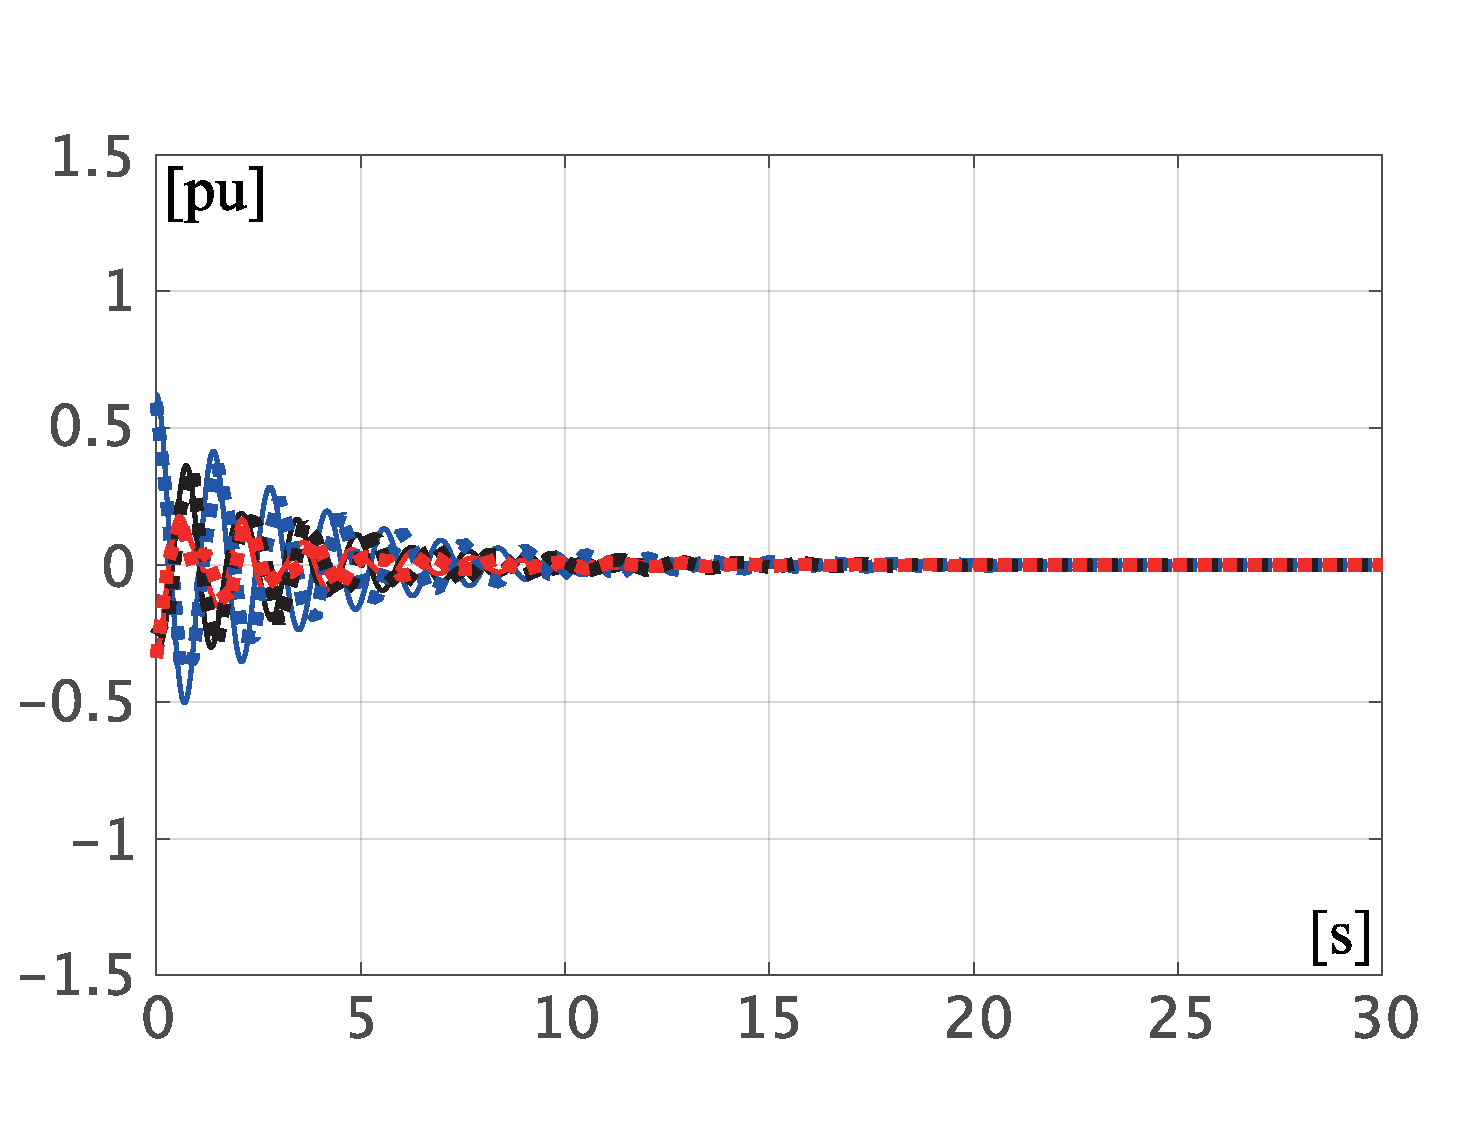
\includegraphics[width = 1.0\linewidth]{figs/Pspa}
    \subcaption{ Solid line:$P^{\rm lin}$, Dotted line:$\hat{P}^{\rm lin}$ }
    \medskip
  \end{minipage}
  }
  \medskip
  \caption{\textbf{Time response when low-dimensional approximation is applied}
  \\  \centering(Blue: Generator 1, Black: Generator 2, Red: Generator 3)}
  \label{fig:timeexsp}
\medskip
\end{figure}

\begin{example}{Low-dimensional approximation for an approximate linear model}
As a reference, the time response of the second-order oscillator system of
Equation \ref{eq:spamodel} for the approximate linear model discussed in Example
\ref{ex:linsyssim} is shown in Figure \ref{fig:timeexsp}. The solid lines
represent the response of the original approximate linear model, while the
dashed lines represent the response of the second-order oscillator system
obtained by applying the low-dimensional approximation of the singular
perturbation system. In addition,

\[
  \Delta \hat{\omega}^{\rm lin}:=\omega_0^{-1} \dot{\hat{\delta}}^{\rm lin},\qquad
  \hat{E}^{\rm lin}:=-A^{-1}B\hat{\delta}^{\rm lin},\qquad
  \hat{P}^{\rm lin}:= L \hat{\delta}^{\rm lin} + C \hat{E}^{\rm lin}
\]

The initial values for the approximate linear model are given by:

\[
  \hat{\delta}^{\rm lin}(0)
  =
  \mat{
  \tfrac{\pi}{6} \\
  0 \\
  0
  },\qquad
  \Delta \hat{\omega}^{\rm lin}(0)
  =
  \mat{
  0 \\
  0 \\
  0
  }
\]

From Figure \ref{fig:timeexsp}, it can be seen that the time response of both
systems matches well in terms of the peak values and decay rates of the
oscillations.
\end{example}

\subsection{Necessary condition for the steady-state stability of the
approximate linear model \advanced}\label{sec:nesconsta}
In the following, we discuss the necessity of the passive power transmission
condition (iii) for the steady-state stability of the approximate linear model
in equation \ref{eq:lindynu0}.  Specifically, we show that the passive power
transmission condition (iii) is a necessary condition for the steady-state
stability of the approximate linear model regardless of the physical constants
of the generator group.

Note that as shown in section \ref{sec:nesconana}, the passive power
transmission condition (i) is a necessary condition for the stability of the
approximate linear model even in the limit where the time constants $(\taudi){i
\in \mathcal{I}{\rm G}}$ are sufficiently small.  This can be verified by the
fact that if the matrix $A$ is unstable, the low-dimensional approximation of
the singular perturbation system in equation \ref{eq:spa} cannot be applied, and
the internal voltage diverges.

When the passive power transmission condition (ii) does not hold, $L_0$ is
generally not symmetric, so a generalized version of the passive power
transmission condition (iii) was introduced to apply it to non-symmetric $L_0$
as well:

\begin{equation}\label{eq:eigreal}
  \bm{\Lambda}(L_0)\subseteq [0,\infty)
\end{equation}

Here, $\bm{\Lambda}(L_0)$ denotes the set of eigenvalues of $L_0$. The condition
in Equation \ref{eq:eigreal} represents that all eigenvalues of $L_0$ are
"non-negative real numbers". In the following, we refer to this generalized
condition as the passive electrical condition (iii)$'$, defined in Definition
\ref{def:passtrans}. Note that when $L_0$ is symmetric, the passive electrical
conditions (iii) and (iii)$'$ are equivalent. The following lemma is proven.

\begin{lemma}[Necessary condition for the small signal stability of a
second-order oscillator system]\label{thm:2ndsys}
Consider the second-order oscillator system given by Equation \ref{eq:spamodel}.
For any initial conditions and any positive definite $(M_i,D_i){i \in
\mathcal{I}{\rm G}}$, the necessary condition for the existence of a constant
$c_0$ such that Equation \ref{eq:delhat0} holds as $t\rightarrow \infty$ is that
the passive power condition (iii)$'$ holds.

\begin{equation}\label{eq:delhat0}
  \lim_{t\rightarrow \infty} \hat{\delta}^{\rm lin}(t)= c_0 \mathds{1}
\end{equation}

\end{lemma}

\begin{proof}
If the passive transmission condition (iii)$'$ does not hold, we show that there
exist positive constants $(M_i,D_i)_{i \in \mathcal{I}_{\rm G}}$ such that
Equation \ref{eq:delhat0} does not hold. For this purpose, we discuss the
following two cases:
\begin{itemize}
  \item[(a)] There exist eigenvalues of $L_0$ with negative real part or purely imaginary part.
  \item[(b)] There exist eigenvalues of $L_0$ with positive real part and nonzero imaginary part.
\end{itemize}

First, let us consider case (a). In what follows, we choose the constant
matrices $M =\omega_0 I$ and $D = \omega_0 dI$. Then, the eigenvalue equation
for Equation \ref{eq:spamodel} is given by:

\begin{equation*}
  \mat{
  0 & I \\
  -L_0 & -d I
  }
  \mat{v\\w}
  =
  \lambda \mat{v\\w}
\end{equation*}

Eliminating $w$ by substitution from this equation, we obtain:

\begin{equation*}
  \left(\lambda^2 I +d \lambda I + L_0
  \right) v =0
\end{equation*}

This eigenvalue equation implies that $v$ is an eigenvector of $L_0$, and for
its eigenvalue $\kappa$, we have:

\begin{equation}\label{eq:lamsq}
  \lambda^2 + d\lambda +\kappa =0
  \qquad
  \Longleftrightarrow
  \qquad
  \lambda = \frac{-d \pm \sqrt{d^2-4\kappa} }{2}
\end{equation}

Therefore, to show that the real part of $\sqrt{d^2 - 4\kappa}$ is greater than
$d$ in case (a), it suffices to prove that $\sqrt{d^2 - 4\kappa}$ has a larger
real part than $d$ in the case where the real part of $\kappa$ is negative or
the real part of $\kappa$ is zero and the imaginary part of $\kappa$ is nonzero.
In general, for any complex number $\bm{z}$, we have:

\begin{equation*}
  \real[\bm{z}] = \sqrt{ \real[\bm{z}^2 ] + (\imag[\bm{z}])^2 }
\end{equation*}

Using this formula with $ \bm{z} = \sqrt{d^2--4\kappa} $, we obtain:

\begin{equation*}
  \real \Bigl[
  \sqrt{d^2 - 4\kappa }
  \Bigr]
  =\sqrt{
  d^2 - 4 \real[\kappa]
  +
  (\imag[ \bm{z} ])^2
  }
\end{equation*}

This value is always greater than $d$ in case (a), where the real part of
$\kappa$ is negative or the real part of $\kappa$ is zero and the imaginary part
of $\kappa$ is nonzero. Therefore, the 2-degree-of-freedom oscillator system in
equation \ref{eq:spamodel} is unstable in case (a).

Next, consider the case (b). Below, it is shown that there exists a positive
definite number $d$ such that the eigenvalue $\lambda$ of Equation
\ref{eq:lamsq} becomes purely imaginary. If the real matrix $L_0$ has complex
eigenvalues, there must be at least one with a negative imaginary part. Denote
this eigenvalue by $\kappa = \alpha + \beta \bm{j}$, where $\alpha>0$ and
$\beta<0$.  It is shown that there exist some $\omega \neq 0$ and $d>0$ that
satisfy

\[
  -d + \sqrt{d^2-4\kappa}  = \omega \bm{j}
\]

Moving $-d$ to the left-hand side and squaring both sides gives:

\[
  -4 (\alpha + \beta \bm{j}) = 2d \omega \bm{j} -\omega^2
\]

This equation is satisfied if we choose $\omega = 2\sqrt{\alpha}$ and
$d=-\tfrac{\beta}{\sqrt{\alpha}}$. Therefore, the second-order oscillator
system has a steady-state oscillatory solution, and Equation \ref{eq:delhat0}
does not hold.
\end{proof}

Lemma \ref{thm:2ndsys} shows that the passive power transfer condition (iii)$'$
is a necessary condition for the steady-state stability of an approximate linear
model for any generator group's physical parameters in the limit of small
internal voltage time constants. Furthermore, Theorem \ref{thm:stasufcon}
demonstrates that when the passive power transfer conditions (i)--(iii) hold,
the approximate linear model is stable for any physical parameters. Based on
these facts, the conclusion of this section is summarized in the following
theorem.

\begin{theorem}[Small signal stability of linearized models]\label{thm:sync}
For any positive parameters $(M_i,D_i,\taudi){i \in \mathcal{I}{\rm G}}$, the
necessary condition for the steady-state stability of the linearized model in
Equation \ref{eq:lindynu0} is that the passive power transmission conditions (i)
and (iii)$'$ in Definition \ref{def:passtrans} hold.

In particular, if the passive power transmission condition (ii) holds, then the
necessary and sufficient condition for the above steady-state stability is that
the passive power transmission conditions (i) and (iii)$'$ hold.
\end{theorem}

We present an analytical example of the small signal stability of the linear
approximate model using Theorem \ref{thm:sync}.

\begin{example}{Small signal stability analysis based on the passive power
transmission conditions}\label{ex:linthm}

Using Theorem \ref{thm:sync}, let's analyze the small signal stability of the
approximate linear model consisting of three generators discussed in Example
\ref{ex:linsyssim}. The physical constants of the generators are set to the same
values as in Example \ref{ex:linsyssim}. Since the passive power transmission
condition (i) is satisfied for all parameters, the region of parameters where
passive power transmission condition (iii)$'$ is not satisfied is overlaid on
Figure \ref{fig:stacheckX}. However, the red region shows eigenvalues of $L_0$
in which the real part is negative, while the purple region shows eigenvalues of
$L_0$ that are complex. The region on the horizontal axis where $\theta_2$ is
zero represents the case where the passive power transmission condition (ii)
holds.

Theorem \ref{thm:sync} shows that the red and purple regions are "dangerous
parameter regions where the approximate linear model will always become unstable
for a certain setting of physical constants." Additionally, when the passive
power transmission condition (ii) holds, i.e., for parameters on the horizontal
axis where $\theta_2$ is zero, it is shown that the approximate linear model
will always be steady-state stable regardless of the values of these constants
as long as $\theta_1$ is set to a non-red value.

The noteworthy point from the result in Figure \ref{fig:stacheckX} is that the
red parameter region accurately captures part or all of the boundary of the blue
parameter region, where the model is steady-state stable under the physical
constants mentioned above. The necessity of the passive power transmission
condition (iii)$'$ shown in Theorem \ref{thm:sync} implies that there is at
least one setting of physical constants for which the approximate linear model
becomes unstable. Therefore, it is not always possible to accurately capture the
parameter region that ensures steady-state stability for specific constants set
in Example \ref{ex:linsyssim}. On the other hand, the fact that part of the
boundary of the blue region is accurately captured suggests that the approximate
linear model is often unstable when $L_0$ has eigenvalues with negative real
parts.

Also, in cases (a) and (b), it can be seen that there is no purple region.  That
is, for all the explored parameters, the eigenvalues of $L_0$ are real numbers.
Generally, unless $\theta_2$ is zero, $L_0$ is an asymmetric matrix, so it is
not obvious that $L_0$ only has real eigenvalues. On the other hand, in cases
(c) and (d) where the admittance matrix is multiplied by $\frac{1}{100}$, it is
also known that $L_0$ has complex eigenvalues when $\theta_1$ and $\theta_2$ are
relatively large. However, in realistic settings, it has been confirmed that
$L_0$ mostly has real eigenvalues.
\end{example}


\begin{figure}[t!]
  \centering
  {
  \begin{minipage}{0.49\linewidth}
    \centering
    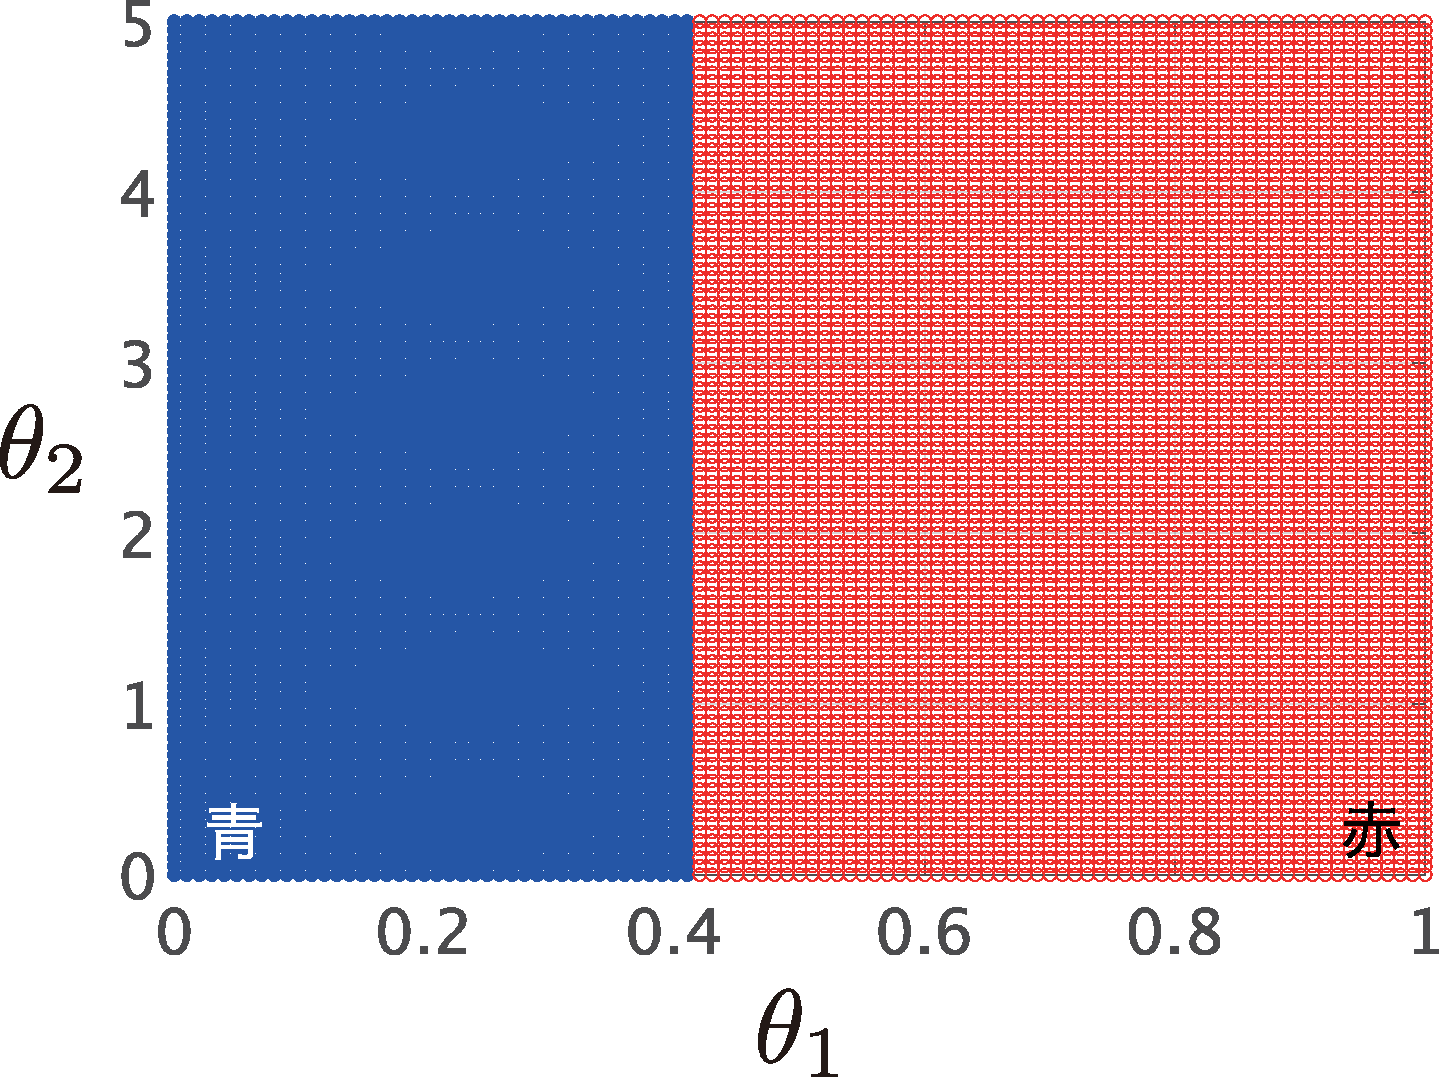
\includegraphics[width = 0.90\linewidth]{figs/Y1D1X}
    \subcaption{ $D=(10,10,10)$,$\bm{Y}=\bm{Y}_0$ }
    \medskip
  \end{minipage}
  \begin{minipage}{0.49\linewidth}
    \centering
    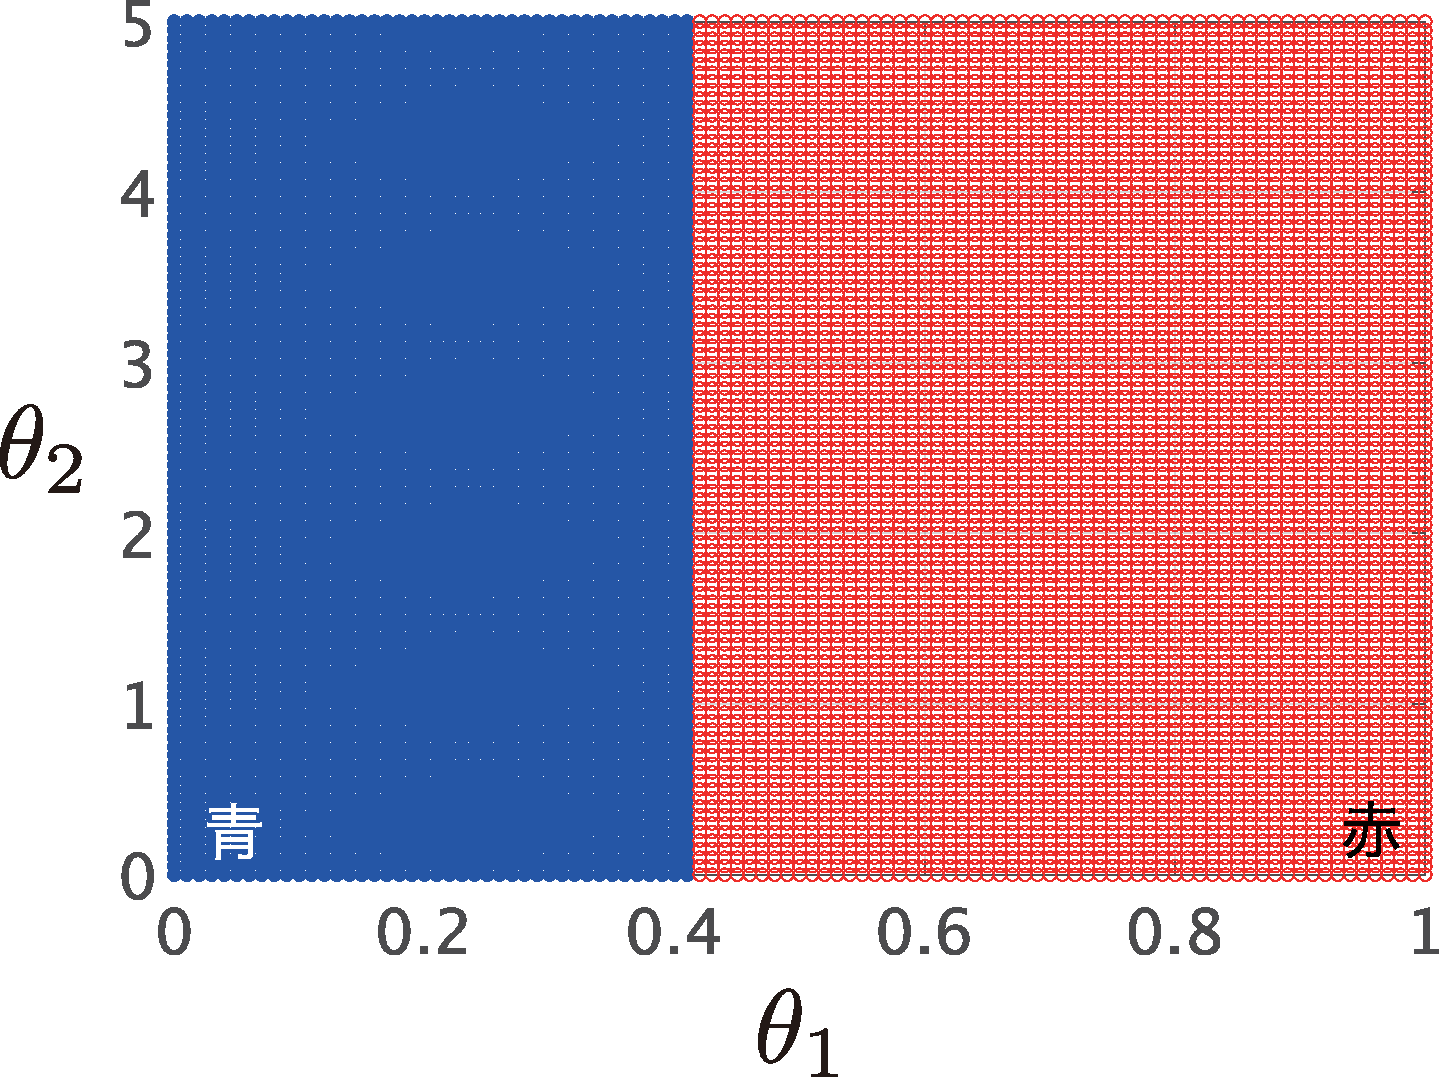
\includegraphics[width = 0.90\linewidth]{figs/Y1D0.01X}
    \subcaption{$D=(0.1,0.1,0.1)$,$\bm{Y}=\bm{Y}_0$ }
    \medskip
  \end{minipage}
}
  \centering
  {
  \begin{minipage}{0.49\linewidth}
      \centering
    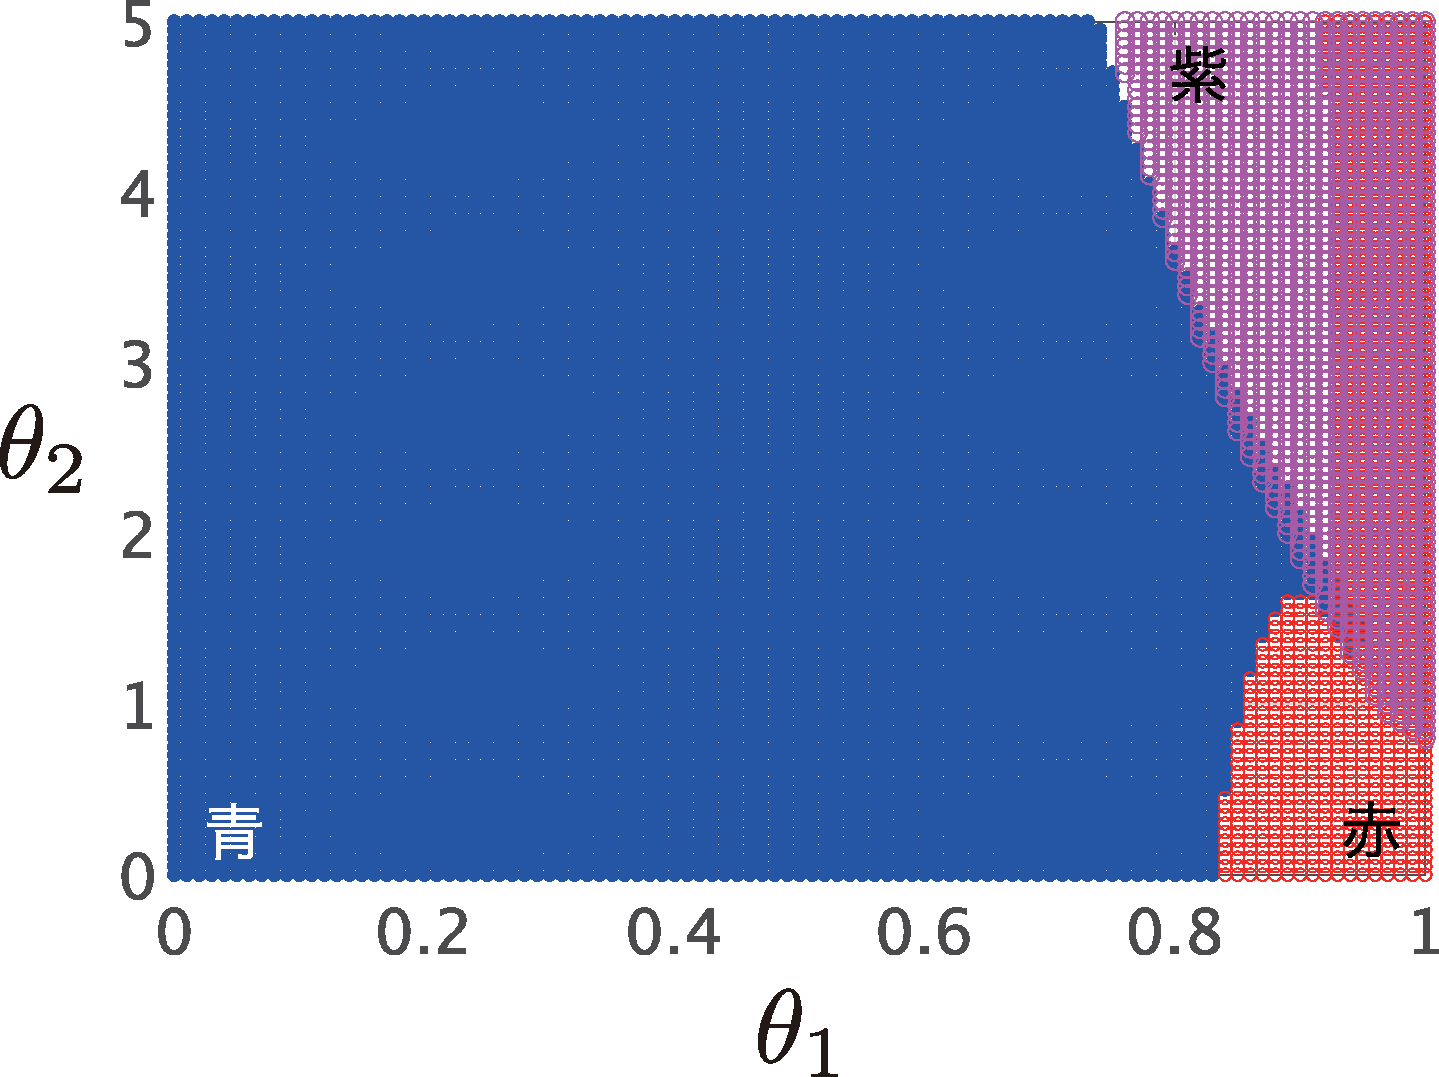
\includegraphics[width = 0.90\linewidth]{figs/Y0.01D1X}
    \subcaption{$D=(10,10,10)$,$\bm{Y}=\tfrac{\bm{Y}_0}{100}$ }
    \medskip
  \end{minipage}
  \begin{minipage}{0.49\linewidth}
    \centering
    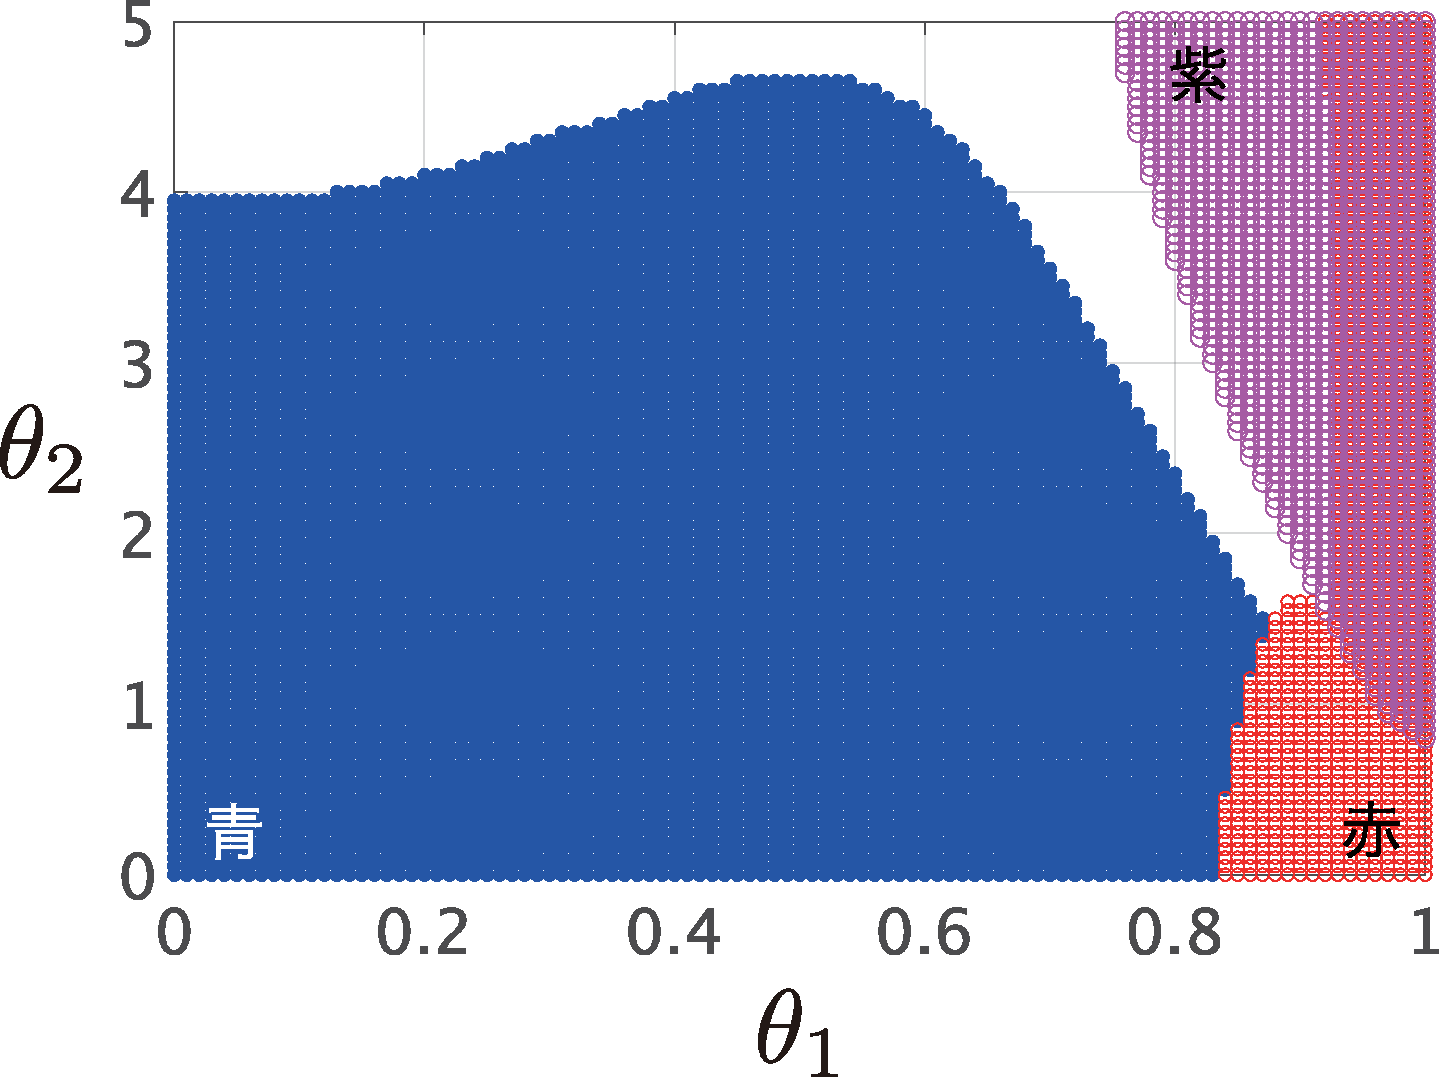
\includegraphics[width = 0.90\linewidth]{figs/Y0.01D0.01X}
    \subcaption{$D=(0.1,0.1,0.1)$,$\bm{Y}=\tfrac{\bm{Y}_0}{100}$ }
    \medskip
  \end{minipage}
}
% \medskip
 \caption{\textbf{Regions of parameters for which the approximate linear model is stable}}
 \label{fig:stacheckX}
\medskip
\end{figure}

%\bibliographystyle{myjunsrt}		% bib style
%\bibliography{reference}	% your bib database


\section*{Mathematical Appendix}
\begin{lemma}\label{lem:prlem}
Consider a stable and square transfer function:

\[
  Q(s)=C(sI-A)^{-1}B + D
\]
where $(A,B)$ is controllable and $(C,A)$ is observable.
The necessary and sufficient condition for $Q(s)$ to be positive real is the
existence of a positive definite symmetric matrix $P$ such that:

\begin{equation*}%\label{eq:prlem}
\mat{
A^{\sf T}P+PA & PB-C^{\sf T} \\
B^{\sf T} P -C & -(D+D^{\sf T})
}\preceq 0
\end{equation*}
\end{lemma}

The proof can be found in \cite[Theorem 5.31]{antoulas2005approximation} or
\cite[Theorem 3]{anderson1967system}, among others. Also,
\cite{kottenstette2010relationships} provides a detailed overview of related
results.


\begin{lemma}\label{lem:nilem}
Consider a stable and square transfer function

\[
  Q(s)=C(sI-A)^{-1}B + D
\]
where $(A,B)$ is controllable and $(C,A)$ is observable.  The necessary and
sufficient condition for $Q(s)$ to be negative imaginary is that $D$ is
symmetric and there exists a positive definite symmetric matrix $P$ such that:

\begin{equation*}
  A^{\sf T}P+PA \preceq 0
  ,\qquad
  -PA^{-1}B = C^{\sf T}
\end{equation*}
\end{lemma}

The proof can be found in \cite[Lemma 7]{xiong2010negative}, among others.
\end{document}
